\documentclass[12pt,letterpaper,oneside]{book} 
%\documentclass[12pt,twoside,letterpaper]{book}
% oneside indica que nao � frente e verso

% ---------------------------------------------------------------------------- %
% Pacotes 
\usepackage[brazil]{babel} 
\usepackage[latin1]{inputenc}
%\usepackage[pdftex]{graphicx}            % usamos arquivos pdf/png como figuras
%\usepackage{color}
%\usepackage{pifont}
\usepackage{amsfonts}
\usepackage{amssymb} 
%\usepackage{setspace}                   % espa�amento flex�vel
%\usepackage[small,compact]{titlesec}    % cabe�alhos dos t�tulos: menores e compactos
\usepackage{indentfirst}                 % indenta��o do primeiro par�grafo
\usepackage{cite}                        % modo de cita��o legal
%\usepackage{subfigure}                  % uso de v�rias figuras numa s�

\usepackage{makeidx}                     % �ndice remissivo
\usepackage[nottoc]{tocbibind}           % acrescentamos a bibliografia/indice/conteudo no Table of Contents
\usepackage{setspace}
%\usepackage[pagebackref,colorlinks=true,urlcolor=red,citecolor=green,linkcolor=blue]{hyperref}

% By David
\usepackage[dvips]{graphicx} 
\usepackage{amsthm}
\usepackage{acronym} 
\usepackage[portugues,ruled,vlined,linesnumbered]{algorithm2e/algorithm2e}
\usepackage{supertabular}

\makeindex  % <== Talvez seja desnecessario

\pagestyle{headings}
\markboth{}{}

% ---------------------------------------------------------------------------- %
% Dimens�es da p�gina (letterpaper)
%\setlength{\paperwidth}{216mm}
%\setlength{\topmargin}{1.3cm}         % deslocamento do topo do texto 
\setlength\oddsidemargin{0cm}
\setlength\evensidemargin{0cm}
\setlength{\parskip}{1.2mm}
%\setlength{\parindent}{4mm}
\setlength{\textwidth}{135mm}          % largura do texto
%\setlength{\parindent}{0pt}
%\setlength{\textheight}{22cm}
%\setlength{\parskip}{0.2cm}


\newcommand{\eb}{\varepsilon}
\newcommand{\mdp}{\langle\mathcal{S,A},p,r,c\rangle}
\newcommand{\ctlstar}{{\sc ctl}$^\star$}
\newcommand{\ctl}{\sc ctl}
\newcommand{\ltl}{\sc ltl}
\newtheorem{Def}{Defini��o}[chapter]
\newtheorem{Teo}{Teorema}[chapter]
\newtheorem{Ex}{Exemplo}[section]
\newtheorem{Tab}{Tabela}[chapter]

\begin{document}
%\hypersetup{
%pdfauthor = {Suelen Goularte Carvalho},
%pdftitle = {Algo Relacionado a Mobile},
%pdfsubject = {Disserta��o de Mestrado},
%pdfkeywords={Mobile, Computa��o Movel, Celular} % <== Precisa rever o que vai colocar aqui !!!
%pdfcreator = {LaTeX with hyperref package},
%}

\frontmatter

\onehalfspacing
\thispagestyle{empty}
\begin{center}
    \vspace*{0.2cm}
    \textbf{\Large{Um conjunto validado de code-smells em Arquiteturas Model-View-Controller no ambiente Android a ser apresentado � CPG para a disserta��o}}\\
	
    \vspace*{1.2cm}
    \Large{Suelen Goularte Carvalho} \\ 
    
    \vskip 2cm
	\textsc{
	Disserta��o apresentada\\[-0.25cm] 
	ao\\[-0.25cm]
	Instituto de Matem�tica e Estat�stica\\[-0.25cm]
	da\\[-0.25cm]
	Universidade de S�o Paulo\\[-0.25cm]
	para\\[-0.25cm]
	obten��o do t�tulo\\[-0.25cm]
	de\\[-0.25cm]
	Mestre em Ci�ncias}
    
    \vskip 1.5cm
    Programa: Ci�ncia da Computa��o\\
    Orientador: Prof. Dr. Marco Aur�lio Gerosa\\

    \vskip 1.5cm
    �rea de Concentra��o: Computa��o M�vel\\
    Orientador: Prof. Dr. Marco Aur�lio Gerosa\\

    \vskip 1cm
	\normalsize{}
	
    \vskip 0.5cm
    \normalsize{S�o Paulo, Julho de 2016}

\end{center}

% P�gina de rosto
\newpage
\thispagestyle{empty}
	\begin{center}
    	\vspace*{0.2 cm}
        \textbf{\Large{Um conjunto validado de code-smells em Arquiteturas Model-View-Controller no ambiente Android a ser apresentado � CPG para disserta��o}}\\
	    \vspace*{2 cm}
	\end{center}

	\vskip 2cm

	\begin{flushright}
	Esta � a vers�o original da disserta��o elaborada pelo\\
	candidato Suelen Goularte Carvalho, tal como\\
	submetida a Comiss�o Julgadora.\\
	\vskip 3cm

	\end{flushright}
	\vskip 4.2cm

	\begin{quote}
	\noindent Comiss�o Julgadora:
	
	\begin{itemize}
		\item {Prof. Dr. Marco Aur�lio Gerosa $-$ IME-USP}
		\item {Prof. Dr. Nome 222 222 $-$ IME-USP}
		\item {Prof. Dr. Nome 333 333 $-$ IME-USP}
	\end{itemize}
	  
	\end{quote}

\newpage
\thispagestyle{empty}
	\vspace*{12cm}
	\vskip 1cm

	\begin{flushright}
	{\small Dedico esta disserta��o de mestrado aos meus\\
	\ldots \\
	\ldots \\
	\ldots .\\}
	\end{flushright}

	\vspace*{1cm}

	\begin{flushright}
	%{\it ``A Estrada vai sempre em frente''} \\
	%$-$ Bilbo Baggins
	\end{flushright}

\pagebreak


\pagenumbering{roman}

\onehalfspacing
\chapter*{Agradecimentos}
\setlength{\parindent}{0mm}

Lorem ipsum dolor sit amet, consectetur adipiscing elit, sed do eiusmod tempor incididunt ut labore et dolore magna aliqua. Ut enim ad minim veniam, quis nostrud exercitation ullamco laboris nisi ut aliquip ex ea commodo consequat. Duis aute irure dolor in reprehenderit in voluptate velit esse cillum dolore eu fugiat nulla pariatur. Excepteur sint occaecat cupidatat non proident, sunt in culpa qui officia deserunt mollit anim id est laborum. \\

Lorem ipsum dolor sit amet, consectetur adipiscing elit, sed do eiusmod tempor incididunt ut labore et dolore magna aliqua. Ut enim ad minim veniam, quis nostrud exercitation ullamco laboris nisi ut aliquip ex ea commodo consequat. \\
%; e a todos os outros que de alguma forma contribu�ram para este momento. \\

%Agrade�o primeiramente
Lorem ipsum dolor sit amet, consectetur adipiscing elit, sed do eiusmod tempor incididunt ut labore et dolore magna aliqua.  \\

Lorem ipsum dolor sit amet, consectetur adipiscing elit, sed do eiusmod tempor incididunt ut labore et dolore magna aliqua. \\

Lorem ipsum dolor sit amet, consectetur adipiscing elit, sed do eiusmod tempor incididunt ut labore et dolore magna aliqua. \\

%%%%%%%%%%%%%%%%%%%%%%%%%%%%%%%%%%%%%%%%%%%%%%%%%%%%%%%%%%%%%%%%%%%%%%%
\setlength{\parindent}{0pt}
\setlength{\textheight}{22cm}
\setlength{\parskip}{0.2cm}

% Para aumentar o espa�amento entre as linhas
\linespread{1.2}
%%%%%%%%%%%%%%%%%%%%%%%%%%%%%%%%%%%%%%%%%%%%%%%%%%%%%%%%%%%%%%%%%%%%%%%

\chapter*{Resumo}

Lorem ipsum dolor sit amet, consectetur adipiscing elit, sed do eiusmod tempor incididunt ut labore et dolore magna aliqua. Ut enim ad minim veniam, quis nostrud exercitation ullamco laboris nisi ut aliquip ex ea commodo consequat. Duis aute irure dolor in reprehenderit in voluptate velit esse cillum dolore eu fugiat nulla pariatur. Excepteur sint occaecat cupidatat non proident, sunt in culpa qui officia deserunt mollit anim id est laborum. \\

Lorem ipsum dolor sit amet, consectetur adipiscing elit, sed do eiusmod tempor incididunt ut labore et dolore magna aliqua. Ut enim ad minim veniam, quis nostrud exercitation ullamco laboris nisi ut aliquip ex ea commodo consequat. \\

Lorem ipsum dolor sit amet, consectetur adipiscing elit, sed do eiusmod tempor incididunt ut labore et dolore magna aliqua. Ut enim ad minim veniam, quis nostrud exercitation ullamco laboris nisi ut aliquip ex ea commodo consequat. Duis aute irure dolor in reprehenderit in voluptate velit esse cillum dolore eu fugiat nulla pariatur. Excepteur sint occaecat cupidatat non proident, sunt in culpa qui officia deserunt mollit anim id est laborum. \\

Lorem ipsum dolor sit amet, consectetur adipiscing elit, sed do eiusmod tempor incididunt ut labore et dolore magna aliqua. Ut enim ad minim veniam, quis nostrud exercitation ullamco laboris nisi ut aliquip ex ea commodo consequat. Duis aute irure dolor in reprehenderit in voluptate velit esse cillum dolore eu fugiat nulla pariatur. Excepteur sint occaecat cupidatat non proident, sunt in culpa qui officia deserunt mollit anim id est laborum. \\

%\cleardoublepage
\noindent \textbf{Palavras-chave:} planejamento em Intelig�ncia Artificial, reparo de plano, replanejamento.

\chapter*{Abstract}

Lorem ipsum dolor sit amet, consectetur adipiscing elit, sed do eiusmod tempor incididunt ut labore et dolore magna aliqua. Ut enim ad minim veniam, quis nostrud exercitation ullamco laboris nisi ut aliquip ex ea commodo consequat. Duis aute irure dolor in reprehenderit in voluptate velit esse cillum dolore eu fugiat nulla pariatur. Excepteur sint occaecat cupidatat non proident, sunt in culpa qui officia deserunt mollit anim id est laborum. \\

Lorem ipsum dolor sit amet, consectetur adipiscing elit, sed do eiusmod tempor incididunt ut labore et dolore magna aliqua. Ut enim ad minim veniam, quis nostrud exercitation ullamco laboris nisi ut aliquip ex ea commodo consequat. \\

Lorem ipsum dolor sit amet, consectetur adipiscing elit, sed do eiusmod tempor incididunt ut labore et dolore magna aliqua. Ut enim ad minim veniam, quis nostrud exercitation ullamco laboris nisi ut aliquip ex ea commodo consequat. Duis aute irure dolor in reprehenderit in voluptate velit esse cillum dolore eu fugiat nulla pariatur. Excepteur sint occaecat cupidatat non proident, sunt in culpa qui officia deserunt mollit anim id est laborum. \\

Lorem ipsum dolor sit amet, consectetur adipiscing elit, sed do eiusmod tempor incididunt ut labore et dolore magna aliqua. Ut enim ad minim veniam, quis nostrud exercitation ullamco laboris nisi ut aliquip ex ea commodo consequat. Duis aute irure dolor in reprehenderit in voluptate velit esse cillum dolore eu fugiat nulla pariatur. Excepteur sint occaecat cupidatat non proident, sunt in culpa qui officia deserunt mollit anim id est laborum. \\

\noindent \textbf{Keywords:} Artificial Intelligence planning, plan repair, replanning.

\onehalfspacing
\tableofcontents

\chapter{Lista de Abreviaturas}

\begin{acronym}

\acro{ADL}{{\it Action Description Language}} % 
\acro{AIPS}{{\it International Artificial Intelligence Planning Systems}}
\acro{BDD}{{\it Binary Decision Diagram}} %  
\acro{CGP}{{\it Conformant Graphplan}} %
\acro{CSP}{{\it Constraint Satisfaction Problems}}
\acro{CWA}{{\it Closed World Assumption}}
\acro{GPG}{{\it Greedy Planning Graph}} %  
\acro{GPS}{{\it General Problem Solver}}
\acro{HTN}{{\it Hierarchical Task Network}} %  
\acro{IPEM}{{\it Integrated Planning, Exe\-cu\-ti\-on, and Mo\-ni\-to\-ring}} %  
\acro{MDP}{{\it Markov Decision Process}} % 
\acro{PDDL}{{\it Problem Domain Definition Language}} %  
\acro{POCL}{{\it Partial Order Causal Link}}
\acro{POMDP}{{\it Partially Observable Markov Decision Process}} % 
\acro{POP}{{\it Partial Order Planner}} %  
\acro{POPR}{{\it Partial Order Plan Repair}} %  
\acro{PRM}{{\it Probabilistic Roadmap Method}} % 
\acro{SIPE}{{\it System for Iteractive Planning and Exe\-cu\-ti\-on Mo\-ni\-to\-ring}} % 
\acro{STN}{{\it Simple Temporal Netwaorking}}
\acro{STRIPS}{{\it Stanford Research Institute Planning System}} % 
\acro{UCPOP}{{\it Partial Order Planner whose step descriptions include Conditional effects and Universal quantification}}
\acro{VHPOP}{{\it Versatile Heuristic Partial Order Planner}}
%\acro{VHPOP-RE}{VHPOP-RE}


%\acro{ADL}{Linguagem de Descri��o de A��o ({\it Action Description Language})} % 
%\acro{AIPS}{Sistemas de Planejamento em Intelig�ncia Artificial ({\it Artificial Intelligence Planning Systems}) }
%\acro{BDD}{Diagrama de Decis�o Bin�ria ({\it Binary Decision Diagram})} %  
%\acro{CGP}{Grafo de Planejamento Conformante ({\it Conformant Graphplan})} %
%\acro{CPU}{Unidade Central de Processamento ({\it Central Processing Unit})}
%\acro{CSP}{Problemas de Satisfa��o de Restri��es ({\it Constraint Satisfaction Problems})}
%\acro{CWA}{Suposi��o de Mundo Fechado ({\it Closed World Assumption})}
%\acro{GPG}{Grafo de Planejamento Guloso ({\it Greedy Planning Graph})} %  
%\acro{GPS}{Solucionador de Problemas Gen�rico ({\it General Problem Solver})}
%\acro{HTML}{Linguagem de Marca��o de Hipertexto ({\it HyperText Markup Language})}
%\acro{HTN}{Rede Hier�rquica de Tarefas ({\it Hierarchical Task Network})} %  
%\acro{IA}{Intelig�ncia Artificial ({\it Artificial Intelligence})} % 
%% ATEN��O: Na dissertacao nao foi utilizado ``\ac{IA}'' pois nao se desejava que a versao em EN estivesse no texto
%\acro{IPEM}{Planejamento Integrado, Execu��o, e Monitoramento ({\it Integrated Planning, Exe\-cu\-ti\-on, and %Mo\-ni\-to\-ring})} %  
%\acro{MDP}{Processo de Decis�o de Markov ({\it Markov Decision Process})} % 
%\acro{PDDL}{Linguagem de Defini��o de Dom�nio de Planejamento ({\it Problem Domain Definition Language})} %  
%% ATEN��O: Na maior parte disserta��o nao foi utilizado ``\ac{PDDL}'' pois nao se desejava que a versao em PT-BR estivesse no %texto. 
% Somente no Ap�ndice deve aparece a verao por extenso
%\acro{POCL}{V�nculos Causais em Ordem Parcial ({\it Partial Order Causal Link})}
%% ATEN��O: Na disserta��o nao foi utilizado ``\ac{POCL}'' pois se desejava mostrar a sigla em outro formato
%\acro{POMDP}{Processo de Decis�o de Markov Parcialmente Observ�vel ({\it Partially Observable Markov Decision Process})} % 
%\acro{POP}{Planejador de Ordem Parcial ({\it Partial Order Planner})} %  
%\acro{POPR}{Reparo de Plano de Ordem Parcial ({\it Partial Order Plan Repair})} %  
%\acro{PRM}{M�todo Probabil�stico de Roteiro ({\it Probabilistic Roadmap Method})} % 
%\acro{RAM}{Mem�ria de Acesso Aleat�rio ({\it Random Access Memory})}
%\acro{SIPE}{Sistema para Planejamento Iterativo e Monitoramento de Execu��o ({\it System for Iteractive Planning and %Exe\-cu\-ti\-on Mo\-ni\-to\-ring})} % 
%\acro{STN}{Rede Temporal Simples ({\it Simple Temporal Netwaorking})}
%\acro{STRIPS}{Instituto Stanford de Pesquisa em Sistemas de Planejamento ({\it Stanford Research Institute Planning System})} %% 
%% ATEN��O: Na dissertacao nao foi utilizado ``\ac{STRIPS}'' pois nao se desejava que a versao em PT-BR estivesse no texto
%\acro{UCPOP}{Planejador de Ordem Parcial com efeitos Condicionais e quantifica��o Universal ({\it Partial Order Planner whose %step descriptions include Conditional effects and Universal quantification})}
%% ATEN��O: Na disserta��o nao foi utilizado ``\ac{UCPOP}'' pois nao se desejava que a versao em PT-BR estivesse no texto
%\acro{UML}{Linguagem de Modelagem Unificada ({\it Unified Modeling Language})}
%\acro{VHPOP}{Planejador de Ordem Parcial com Versatilidade Heur�stica ({\it Versatile Heuristic Partial Order Planner})}
%%\acro{VHPOP-RE}{VHPOP-RE}

\end{acronym}


\chapter{Lista de S�mbolos}

\begin{supertabular}{ll}


$\Sigma$ & Sistema de transi��o de estados \\
$\Sigma'$ & Sistema de transi��o de estados restrito (est�tico e determin�stico) \\
$\Pi$ & Problema de planejamento \\

$\epsilon$ & Evento nulo \\
$\eta$ & Fun��o de observa��o \\
$\gamma$ & Fun��o de transi��o de estados \\
$\gamma(s, a)$ & Progress�o, conjunto de estados resultantes da aplica��o de $a$ a $s$ \\
$\gamma^{-1}(s, a)$ & Regress�o, conjunto de estados que levam a $s$ com a aplica��o de $a$ \\
$\pi$ & Plano \\

$2^S$ & Conjunto pot�ncia de $S$ \\

$\mathcal{A}$ & Conjunto de todas as a��es poss�veis \\
$\mathcal{C}$ & Conjunto de s�mbolos de constantes \\
$\mathcal{D}$ & Dom�nio de planejamento, conjunto de operadores \\
$\mathcal{E}$ & Conjunto de eventos \\
$\mathcal{H}$ & Hist�rico de refinamentos \\
$\mathcal{O}$ & Conjunto de todas as observa��es poss�veis \\
$\mathcal{P}$ & Plano parcial \\
$\mathcal{R}$ & Estrat�gia de refinamento \\
$\mathcal{S}$ & Conjunto de todos os estados poss�veis \\

$E_p$ & Estrutura do plano \\
$G$ & Conjunto de estados meta \\
$O$ & Conjunto de observa��es, sub-conjunto de $\mathcal{S}$ \\
$P$ & Problema de planejamento \\
$S$ & Conjunto de estados, sub-conjunto de $\mathcal{S}$ \\
$S_0$ & Conjunto de estados iniciais \\
$S_g$ & Conjunto de estados objetivos \\

$\mathsf{no\mbox{-}op}$ & A��o nula \\

$a$ & A��o de $\mathcal{A}$ \\
$e$ & Evento de $\mathcal{E}$\\

$o$ & Observa��o de $\mathcal{O}$ \\
$s$ & Estado de $\mathcal{S}$ \\
$s_0$ & Estado inicial \\

%$\langle \ldots \rangle$ & tupla \\
%$( \ldots )$ & lista \\
%$\{ \ldots \}$ & conjunto \\
%
%$\cup$ & uni�o de conjuntos \\
%$\cap$ & interse��o de conjuntos \\
%$\setminus$ & subtra��o de conjuntos \\


\end{supertabular}


\listoffigures
\listofalgorithms

\mainmatter

%%%%%%%%%%%%%%%%%%%%%%%%%%%%%%%%%%%%%%%%%%%%%%%%%%%%%%%%%%%%%%%%%%%%%%%%%
\onehalfspacing

%%%%%%%%%%%%%%%%%%%%%%%%%%%%%%%%%%%%%%%%%%%%%%%%%%%%%%%%%%%%%%%%%%%%%%%
\setlength{\parindent}{0pt}
\setlength{\textheight}{22cm}
\setlength{\parskip}{0.2cm}

% Para aumentar o espa�amento entre as linhas
\linespread{1.2}
%%%%%%%%%%%%%%%%%%%%%%%%%%%%%%%%%%%%%%%%%%%%%%%%%%%%%%%%%%%%%%%%%%%%%%%

\chapter{Introdu��o}

Planejamento\index{planejamento} � um componente importante do comportamento racional pois trata-se de um processo de s�ntese que seleciona e organiza a��es antecipando seus efeitos. Este processo busca satisfazer, da melhor forma poss�vel, um conjunto de metas pr�-definidas. \\

Muitas tarefas\index{tarefa} humanas necessitam de planejamento. Lorem ipsum dolor sit amet, consectetur adipiscing elit, sed do eiusmod tempor incididunt ut labore et dolore magna aliqua. Ut enim ad minim veniam, quis nostrud exercitation ullamco laboris nisi ut aliquip ex ea commodo consequat. Duis aute irure dolor in reprehenderit in voluptate velit esse cillum dolore eu fugiat nulla pariatur. Excepteur sint occaecat cupidatat non proident, sunt in culpa qui officia deserunt mollit anim id est laborum. \cite{RomanWeerdt2004}. Lorem ipsum dolor sit amet, consectetur adipiscing elit, sed do eiusmod tempor incididunt ut labore et dolore magna aliqua. O Exemplo \ref{ex:viagem_curitiba} ilustra um problema real de planejamento. \\

\begin{Ex}
\label{ex:viagem_curitiba}
Lorem ipsum dolor sit amet, consectetur adipiscing elit, sed do eiusmod tempor incididunt ut labore et dolore magna aliqua.

\begin{itemize}
\item Lorem ipsum dolor sit amet, consectetur adipiscing elit, sed do eiusmod tempor incididunt ut labore et dolore magna aliqua.
\item Lorem ipsum dolor sit amet, consectetur adipiscing elit, sed do eiusmod tempor incididunt ut labore et dolore magna aliqua.
\item Lorem ipsum dolor sit amet, consectetur adipiscing elit, sed do eiusmod tempor incididunt ut labore et dolore magna aliqua.
\end{itemize}
\end{Ex}

Um plano simplificado para o problema do Exemplo \ref{ex:viagem_curitiba}, Lorem ipsum dolor sit amet, consectetur adipiscing elit, sed do eiusmod tempor incididunt ut labore et dolore magna aliqua.\\

Lorem ipsum dolor sit amet, consectetur adipiscing elit, sed do eiusmod tempor incididunt ut labore et dolore magna aliqua. \\

\begin{Ex}
Um exemplo de falha\index{falha}, Lorem ipsum dolor sit amet, consectetur adipiscing elit, sed do eiusmod tempor incididunt ut labore et dolore magna aliqua.
\end{Ex}

Quando o plano falha h�, basicamente, duas solu��es: identificar a situa��o como um novo problema e criar um novo plano para a situa��o ({\it replanejamento}\index{replanejamento}), ou tentar reparar o plano existente ({\it reparo de plano}\index{reparo!de plano}). Um argumento a favor do reparo de planos \cite{Roman2005phd} � considerar a quantidade de trabalho j� executada e pensar na quantidade de trabalho que ser� exigida para se criar um novo plano: lorem ipsum dolor sit amet, consectetur adipiscing elit, sed do eiusmod tempor incididunt ut labore et dolore magna aliqua. No entanto, a tarefa de reparo\index{reparo}, no pior caso, pode consumir mais trabalho do que um replanejamento\index{replanejamento} completo \cite{Bernhard1993} .\\

Lorem ipsum dolor sit amet, consectetur adipiscing elit, sed do eiusmod tempor incididunt ut labore et dolore magna aliqua. \index{heur�stica} e simula��es.

\subsection*{Lorem ipsum dolor sit amet}\index{Lorem!ipsum}


Sed ut perspiciatis unde omnis iste natus error sit voluptatem accusantium doloremque laudantium, totam rem aperiam, eaque ipsa quae ab illo inventore veritatis et quasi architecto beatae vitae dicta sunt explicabo. Nemo enim ipsam voluptatem quia voluptas sit aspernatur aut odit aut fugit, sed quia consequuntur magni dolores eos qui ratione voluptatem sequi nesciunt. Neque porro quisquam est, qui dolorem ipsum quia dolor sit amet, consectetur, adipisci velit, sed quia non numquam eius modi tempora incidunt ut labore et dolore magnam aliquam quaerat voluptatem. Ut enim ad minima veniam, quis nostrum exercitationem ullam corporis suscipit laboriosam, nisi ut aliquid ex ea commodi consequatur? Quis autem vel eum iure reprehenderit qui in ea voluptate velit esse quam nihil molestiae consequatur, vel illum qui dolorem eum fugiat quo voluptas nulla pariatur?\\

At vero eos et accusamus et iusto odio dignissimos ducimus qui blanditiis praesentium voluptatum deleniti atque corrupti quos dolores et quas molestias excepturi sint occaecati cupiditate non provident, \cite{Malik2004}. At vero eos et accusamus et iusto odio dignissimos ducimus qui blanditiis praesentium voluptatum deleniti atque corrupti quos dolores et quas molestias excepturi sint occaecati cupiditate non provident, \cite{Richard1971, Mason1993}, \cite{Dana1995} xyz, abc e def ghi \cite{B.1999} \cite{Rabideau1999}, entre outros.\\
 

\subsection*{Sed ut perspiciatis unde omniso}\index{Lorem!perspiciatis}

At vero eos et accusamus et iusto odio dignissimos ducimus qui blanditiis praesentium voluptatum deleniti atque corrupti quos dolores et quas molestias excepturi sint occaecati cupiditate non provident, similique sunt in culpa qui officia deserunt mollitia animi, id est laborum et dolorum fuga. Et harum quidem rerum facilis est et expedita distinctio. Nam libero tempore, cum soluta nobis est eligendi optio cumque nihil impedit quo minus id quod maxime placeat facere possimus, omnis voluptas assumenda est, omnis dolor repellendus. Temporibus autem quibusdam et aut officiis debitis aut rerum necessitatibus saepe eveniet ut et voluptates repudiandae sint et molestiae non recusandae. Itaque earum rerum hic tenetur a sapiente delectus, ut aut reiciendis voluptatibus maiores alias consequatur aut perferendis doloribus asperiores repellat.\index{espa�o!de busca}. Entre elas, eabcdef ghijt\index{heur�stica!independente do dom�nio} para reduzir o custo da busca \cite{DBLP:journals/ai/BonetG01, DBLP:journals/jair/HoffmannN01}, Sed ut perspiciatis unde omnis iste natus error sit voluptatem accusantium doloremque laudantium, totam rem aperiam, eaque ipsa quae ab illo inventore veritatis et \cite{Nau1999} abcdefg. \\

\section{Motiva��o}\index{motiva��o}

A motiva��o desta disserta��o surgiu da possibilidade de aplica��o da t�cnica de Sed ut perspiciatis unde omnis iste natus error sit voluptatem accusantium doloremque laudantium, totam rem aperiam, eaque ipsa quae ab illo inventore veritatis et quasi architecto beatae vitae dicta sunt explicabo. Nemo enim ipsam voluptatem quia voluptas sit aspernatur aut odit aut fugit, sed quia consequuntur magni dolores eos qui ratione voluptatem sequi nesciunt. 

\section{Objetivos}

Sed ut perspiciatis unde omnis iste natus error sit voluptatem accusantium doloremque laudantium, totam rem aperiam, eaque ipsa quae ab illo inventore veritatis et quasi architecto beatae vitae dicta sunt explicabo. Nemo enim ipsam voluptatem quia voluptas sit aspernatur aut odit aut fugit, sed quia consequuntur magni dolores eos qui ratione voluptatem sequi nesciunt. \\

\section{Organiza��o}\index{organiza��o}

No Cap�tulo \ref{cap:modelo_conceitual_planejamento} � apresentado um modelo conceitual . O Cap�tulo \ref{cap:planejamento_classico} trata de planejamento cl�ssico Sed ut perspiciatis unde omnis iste natus error sit voluptatem accusantium doloremque laudantium, totam rem aperiam, eaque ipsa quae ab illo inventore veritatis et quasi architecto beatae vitae dicta sunt explicabo. Nemo enim ipsam voluptatem quia voluptas sit aspernatur aut odit aut fugit, sed quia consequuntur magni dolores eos qui ratione voluptatem sequi nesciunt.  No Cap�tulo \ref{cap:planejamento_nao-classico}, � discutido a situa��o em que um Sed ut perspiciatis unde omnis iste natus error sit voluptatem accusantium doloremque laudantium, totam rem aperiam, eaque ipsa quae ab illo inventore veritatis et quasi architecto beatae vitae dicta sunt explicabo. Nemo enim ipsam voluptatem quia voluptas sit aspernatur aut odit aut fugit, sed quia consequuntur magni dolores eos qui ratione voluptatem sequi nesciunt.  O Cap�tulo \ref{cap:reparo_de_plano_por_refinamento_reverso} Sed ut perspiciatis unde omnis iste natus error sit voluptatem accusantium doloremque laudantium, totam rem aperiam, eaque ipsa quae ab illo inventore veritatis et quasi architecto beatae vitae dicta sunt explicabo. Nemo enim ipsam voluptatem quia voluptas sit aspernatur aut odit aut fugit, sed quia consequuntur magni dolores eos qui ratione voluptatem sequi nesciunt. Finalmente, o Cap�tulo \ref{cap:conclusao} encerra esta disserta��o com as conclus�es, contribui��es e recomenda��es para trabalhos futuros. \\


 % 
%%%%%%%%%%%%%%%%%%%%%%%%%%%%%%%%%%%%%%%%%%%%%%%%%%%%%%%%%%%%%%%%%%%%%%%
\setlength{\parindent}{0pt}
\setlength{\textheight}{22cm}
\setlength{\parskip}{0.2cm}

% Para aumentar o espa�amento entre as linhas
\linespread{1.2}
%%%%%%%%%%%%%%%%%%%%%%%%%%%%%%%%%%%%%%%%%%%%%%%%%%%%%%%%%%%%%%%%%%%%%%%

\chapter{Modelo para planejamento}
\label{cap:modelo_conceitual_planejamento}

At vero eos et accusamus et iusto odio dignissimos ducimus\index{ducimus},  qui blanditiis praesentium voluptatum deleniti atque corrupti quos dolores et quas molestias excepturi sint occaecati cupiditate non provident, similique sunt in culpa qui officia deserunt mollitia animi, id est laborum et dolorum fuga. Et harum quidem rerum facilis est et expedita distinctio. Nam libero tempore, cum soluta nobis est eligendi optio cumque nihil impedit quo minus id quod maxime placeat facere possimus, omnis voluptas assumenda est, omnis dolor repellendus. Temporibus autem quibusdam et aut officiis debitis aut rerum necessitatibus saepe eveniet ut et voluptates repudiandae sint et molestiae non recusandae. Itaque earum rerum hic tenetur a sapiente delectus, ut aut reiciendis voluptatibus maiores alias consequatur aut perferendis doloribus asperiores repellat..

\section{Modelo conceitual para planejamento}

At vero eos et accusamus et iusto odio dignissimos ducimus qui blanditiis praesentium voluptatum deleniti atque corrupti quos dolores et quas molestias excepturi sint occaecati cupiditate non provident.\\

\begin{Def}[Sistema de transi��o de estados]
Um sistema de transi��o de estados � uma 4-tupla $\Sigma\ =\ (\mathcal{S},\ \mathcal{A},\ \mathcal{E},\ \gamma)$ \cite{Malik2004}:

\begin{itemize}

\item $\mathcal{S}\ =\ \{s_1,\ s_2,\ \ldots\}$ � um conjunto finito de estados, recursivamente numer�vel;

\item $\mathcal{A}\ =\ \{a_1,\ a_2, \ \ldots\}$ � um conjunto finito de a��es, recursivamente numer�vel;

\item $\mathcal{E}\ =\ \{e_1,\ e_2, \ \ldots\}$ � um conjunto finito de eventos, recursivamente numer�vel, que aqui ser�o chamados de {\it a��es ex�genas\index{a��o!ex�gena}} (ou {\it eventos ex�genos\index{evento!ex�geno}}); 

\item $\gamma:\ \mathcal{S}\ \times\  \mathcal{A}\ \times\ \mathcal{E}\ \to\ 2^s$ � uma fun��o de transi��o de estado.

\end{itemize}

\end{Def}

At vero eos et accusamus et iusto odio dignissimos ducimus qui blanditiis praesentium voluptatum deleniti atque corrupti quos dolores et quas molestias excepturi sint occaecati cupiditate non provident.

\begin{figure}[ht!]
	\centering
	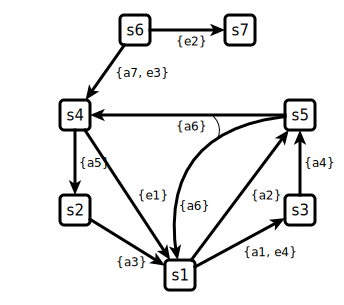
\includegraphics[scale=0.80]{./img/grafo_transicao_estado.ps}
	\caption[Exemplo de sistema de transi��o de estado]{Exemplo de sistema de transi��o de estados.}
	\label{fig:sistemaTransicaoEstado}
\end{figure}

At vero eos et accusamus et iusto odio dignissimos ducimus qui blanditiis praesentium voluptatum deleniti atque corrupti quos dolores et quas molestias excepturi sint occaecati cupiditate non provident.

{\it Eventos \index{evento}} s�o transi��es {\it contingentes} \index{transi��o!contingente}, aqui chamados de eventos ex�genos\index{evento!ex�geno} (ou a��es ex�genas\index{a��o!ex�gena}), isto �, a��es que n�o s�o controladas pelo executor do plano. Estas a��es devem ser levadas em conta pelo agente de planejamento, mas n�o est�o sob seu controle. Se $e$ � um evento e $\gamma(s,e)$ n�o � vazio, ent�o $e$ possivelmente ocorrer� quando o sistema estiver no estado $s$; e sua ocorr�ncia em $s$ levar� o sistema a algum estado em $\gamma(s,e)$. Como o estado exato n�o pode ser previs�vel pelo agente planejador, dizemos que este � um tipo de planejamento sob incerteza. \\
%\footnote{Eventos ex�genos podem tamb�m ser modelados. Por�m, neste trabalho, o agente planejador n�o possui representa��o interna deste modelo} \\ 

Podem existir v�rios modelos que definem a sem�ntica da fun��o de transi��o\index{fun��o!de transi��o} $\gamma:\ \mathcal{S}\ \times\ \mathcal{A}\ \times\ \mathcal{E}\ \to\ 2^s$. O modelo de Markov\index{modelo!de Markov} sup�e que nenhuma a��o possa ser executada em estados em que ocorram eventos e vice-versa. Deste modo, $\mathcal{S}$ � dividido em {\it estados de a��o\index{estado!de a��o}} e {\it estados de evento\index{estado!de evento}} \cite{Sven1995}. Um modelo alternativo sup�e que a��es possam competir com eventos no mesmo estado. Isto �, se for aplicada a a��o $a$ ao estado $s$ e $\gamma(s,e)$ n�o � vazio, ent�o o pr�ximo estado pode ser qualquer elemento de $\gamma(s,a,e)$. \\

Dado um sistema de transi��o\index{sistema!de transi��o} de estado $\Sigma$, o prop�sito do planejamento � selecionar uma seq��ncia de a��es que, quando executadas no estado inicial, permitam alcan�ar um objetivo. Chama-se de {\it plano\index{plano}} a estrutura que representa a seq��ncia de a��es. O objetivo pode ser especificado de v�rias formas diferentes:

\begin{itemize}

\item As especifica��es mais simples consistem em um {\it estado-objetivo} $s_g$ ou um conjunto de estados objetivo\index{estado!objetivo} $S_g$. Neste caso, o objetivo � alcan�ado quando qualquer se\-q��n\-ci\-a de transi��es de estado termina em um dos estados-objetivo.

\item O objetivo pode satisfazer alguma condi��o de acordo com a se\-q��n\-ci\-a de estados a ser seguida pelo sistema. Por exemplo, exigir que estados sejam evitados, especificar estados em que o sistema dever� passar necessariamente durante a execu��o do plano e estados nos quais ele dever� permanecer.

\item Em alguns dom�nios � poss�vel definir uma fun��o de utilidade\index{fun��o!de utilidade} ligada aos estados, com penalidades\index{penalidades} e recompensas\index{recompensas}. Nesse caso o objetivo � otimizar alguns componentes da fun��o destas utilidades (por exemplo, soma ou m�ximo) conforme a se\-q��n\-ci\-a de estados seguidos pelo sistema.

\item Outra alternativa � especificar o objetivo como tarefas\index{tarefa} que o sistema dever� executar. Estas tarefas podem ser recursivamente decompostas como conjuntos de a��es mais simples.

\end{itemize}

A Figura 2.2
%TODO: ~\ref{fig:modeloConceitualPlanejamento} 
mostra um modelo conceitual do uso de um planejador em um ambiente. Este modelo � descrito por meio da intera��o entre tr�s componentes:

\begin{enumerate}

\item O {\it ambiente\index{ambiente}} denominado $\Sigma$ possui uma din�mica que pode ser modelada por meio da fun��o de transi��o\index{fun��o!de transi��o} de estado $\gamma$, de acordo com a ocorr�ncia dos eventos e das a��es.

\item Um {\it controlador\index{controlador}}, dado como entrada a observa��o do estado em que se encontra o sistema e um plano, fornece como sa�da uma a��o $a$.

\item Um {\it planejador\index{planejador}} que, dado como entrada um modelo do ambiente $\Sigma$\footnote{No decorrer do texto o modelo do ambiente $\Sigma$ ser� tratado apenas por ambiente $\Sigma$ ou, algumas vezes, por sistema $\Sigma$ (de transi��o de estado).} (dom�nio), um estado inicial\index{estado!inicial} e um objetivo, sintetiza um plano que satisfaz o objetivo.

\end{enumerate}

\begin{figure}[ht!]
	\centering
	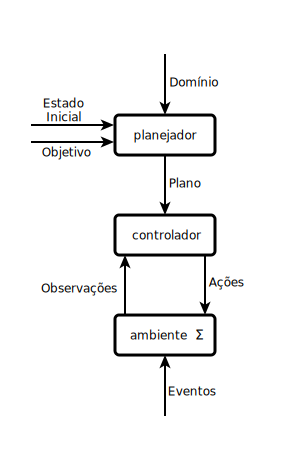
\includegraphics[scale=0.80]{./img/modelo_planejamento.ps}
	\caption[Modelo conceitual para planejamento]{Modelo conceitual para planejamento \cite{Malik2004}.}
	\label{fig:modeloConceitualPlanejamento}
\end{figure}

\subsection{Modelo conceitual para planejamento din�mico}

Um elemento importante deste modelo � a observa��o\index{observa��o} do controlador sobre o estado atual do sistema durante a execu��o de um plano. Em geral, esta informa��o n�o � completa. O conhecimento parcial sobre o estado pode ser modelado como uma fun��o de observa��o\index{fun��o!observa��o} $\eta:\ \mathcal{S}\ \to\ \mathcal{O}$, que mapeia $\mathcal{S}$ em um conjunto discreto $\mathcal{O}\ =\ \{o_1,\ o_2,\ \ldots\}$ de observa��es poss�veis. \\

Neste modelo, o controlador executa suas tarefas com a din�mica do sistema de transi��o de estado e, portanto, diz-se que ele funciona {\it online} com o ambiente. Por outro lado, o planejador n�o est� diretamente conectado ao ambiente (funcionamento {\it offline\index{offline}}).\\
%TODO: ~\ref{fig:modeloConceitualPlanejamento}. \\


Na maior parte das vezes, h� diferen�as entre o sistema f�sico\index{sistema!f�sico} ($\Sigma$) a ser controlado e seu modelo. Em geral, o planejamento depende das restri��es\index{restri��es} impostas pelo modelo\index{modelo} de $\Sigma$. Sup�e-se que o controlador seja robusto o suficiente para lidar com as diferen�as entre $\Sigma$ e o mundo real\index{mundo!real}. Lidar com observa��es exige mecanismos de controle mais complexos do que apenas identificar o estado e aplicar a a��o correspondente. Um modelo conceitual mais realista intercala planejamento com execu��o e mecanismos de replanejamento\index{replanejamento} ou reparo de plano\index{reparo!de plano}. Neste caso � necess�ria uma liga��o mais pr�xima entre o planejador e o controlador: o controlador deve ser capaz de devolver ao planejador o status da execu��o do planejamento a fim de comunicar eventuais falhas\index{falha} no plano, como � ilustrado na Figura 2.3 por meio da liga��o entre controlador e planejador, rotulada por {\it status de execu��o}.\\
%TODO: ~\ref{fig:modeloConceitualPlanejamentoDinamico}. \\

\begin{figure}[ht!]
	\centering
	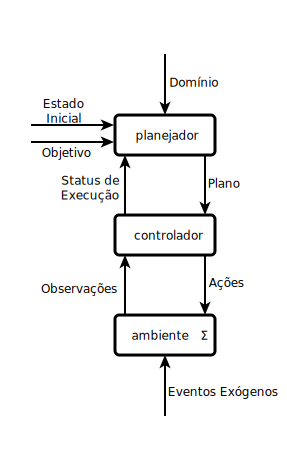
\includegraphics[scale=0.80]{./img/modelo_planejamento_dinamico.ps} 
	\label{fig:modeloConceitualPlanejamentoDinamico}
	\caption[Modelo conceitual para planejamento com execu��o]{Modelo conceitual para planejamento com execu��o \cite{Malik2004}.}
\end{figure} 

Neste trabalho ser� implementado um sistema que ora funcionar� como um sistema de planejamento, quando ainda n�o existir um plano, ora como um sistema de reparo, que depender� da informa��o transmitida pelo controlador (status de execu��o). Esta informa��o poder� ser de dois tipos:

\begin{enumerate}
 \item O plano foi executado inteiramente com sucesso.

\item O plano foi parcialmente executado e, nesse caso, o mesmo � devolvido com as indica��es das a��es que j� foram realizadas e da a��o cuja execu��o falhou. 
\end{enumerate}

No caso de falha (caso 2), o sistema de reparo � ent�o chamado para: (1) adicionar a��es ou (2) remover a��es do plano a fim de torn�-lo novamente execut�vel, garantindo que este atinja as metas originais com pequenas altera��es. % 
%%%%%%%%%%%%%%%%%%%%%%%%%%%%%%%%%%%%%%%%%%%%%%%%%%%%%%%%%%%%%%%%%%%%%%%
\setlength{\parindent}{0pt}
\setlength{\textheight}{22cm}
\setlength{\parskip}{0.2cm}

% Para aumentar o espa�amento entre as linhas
\linespread{1.2}
%%%%%%%%%%%%%%%%%%%%%%%%%%%%%%%%%%%%%%%%%%%%%%%%%%%%%%%%%%%%%%%%%%%%%%%

\chapter{Planejamento cl�ssico}
\label{cap:planejamento_classico}

Neste cap�tulo define-se o problema de planejamento cl�ssico\index{planejamento!cl�ssico} como um modelo simplificado para a tarefa de planejamento, que serve como base para futuras extens�es de algoritmos para problemas mais gerais de planejamento. Apresenta-se, tamb�m, um algoritmo bastante conhecido para planejamento cl�ssico que emprega o m�todo de busca por refinamento de planos. \\

\section{Modelo restrito}

O modelo conceitual\index{modelo!conceitual} descrito no Cap�tulo \ref{cap:modelo_conceitual_planejamento} n�o foi proposto como um modelo operacional\index{modelo!operacional}. Pelo contr�rio, ele � usado como refer�ncia para a constru��o de sistemas de planejamento\index{sistema!de planejamento}. Por meio dele � poss�vel fazer diferentes suposi��es restritivas\index{suposi��es restritivas} sobre o ambiente em que se deseja planejar \cite{Malik2004}:

\begin{itemize}

\item {\bf Suposi��o A0 ($\Sigma$ finito)}. O ambiente $\Sigma$ tem um conjunto finito de estados.

\item {\bf Suposi��o A1 ($\Sigma$ completamente observ�vel)}. O sistema $\Sigma$ � completamente observ�vel\index{completamente observ�vel}. Neste caso, a fun��o observa��o\index{fun��o!observa��o} $\eta$ � a fun��o identidade\index{fun��o!identidade}.

\item {\bf Suposi��o A2 ($\Sigma$ determin�stico)}. O sistema $\Sigma$ � determin�stico\index{determin�stico}, isto �, para cada estado $s$ e para cada evento ou a��o $u,\ |\gamma(s,u)|\ \le\ 1$. Se uma a��o � aplic�vel a um estado, sua execu��o leva um sistema determin�stico\index{sistema!determin�stico} a um outro estado �nico, possivelmente com a ocorr�ncia de um evento ex�geno.

\item {\bf Suposi��o A3 ($\Sigma$ est�tico)}. O sistema $\Sigma$ � est�tico, ou seja, o conjunto de eventos $E$ � vazio. $\Sigma$ permanece no mesmo estado at� que o controlador aplique alguma a��o selecionada pelo planejador.
 
\item {\bf Suposi��o A4 (objetivos restritos)}. O planejador manipula apenas objetivos restritos\index{objetivo!restrito} que s�o especificados como um estado objetivo expl�cito $s_g$ ou um conjunto de estados objetivos $S_g$; sendo que o objetivo � obter qualquer seq��ncia de transi��es de estado que termine em um dos estados objetivos.

\item {\bf Suposi��o A5 (planejamento seq�encial)}. Um plano solu��o para um problema de planejamento � uma seq��ncia finita de a��es de ordem total\index{ordem!total} ou parcial\index{ordem!parcial}. 

\item {\bf Suposi��o A6 (tempo impl�cito)}. A��es e eventos n�o t�m dura��o; s�o transi��es de estado instant�neas. Esta suposi��o est� intr�nseca a um sistema de transi��o de estado, que n�o representa tempo explicitamente.

\item {\bf Suposi��o A7 (planejamento offline)}. O planejador n�o considera qualquer mudan�a que possa ocorrer em $\Sigma$ {\it enquanto} estiver planejando; planeja-se para o estado inicial e o objetivo, independentemente das poss�veis falhas na execu��o do plano.

\end{itemize}

Uma vez que o sistema � determin�stico\index{determin�stico}, se $\gamma$ for aplic�vel em $s$, ent�o $\gamma(s,a)$ corresponde a um �nico estado $s'$. Para simplificar a nota��o, descreve-se $\gamma(s,a)\ =\ s'$ em vez de $\gamma(s,a)\ =\ \{s'\}$. Para este tipo de sistema, um planejamento � uma seq��ncia $\{a_1,\ a_2,\ \ldots,\ a_k\}$, tal que $\gamma(\gamma(\ldots$ $\gamma(\gamma(s_0,$ $a_1),$ $a_2),$ $\ldots,$ $a_{k-1}),$ $a_k)$ � um estado objetivo. Um exemplo de um grafo de transi��es de estados em um {\it modelo restrito}, pode ser observado na Figura ~\ref{fig:sistemaTransicaoEstadoMundoBlocos} \cite{Lago2002}.

%\begin{figure}[ht!]
%	\centering
%	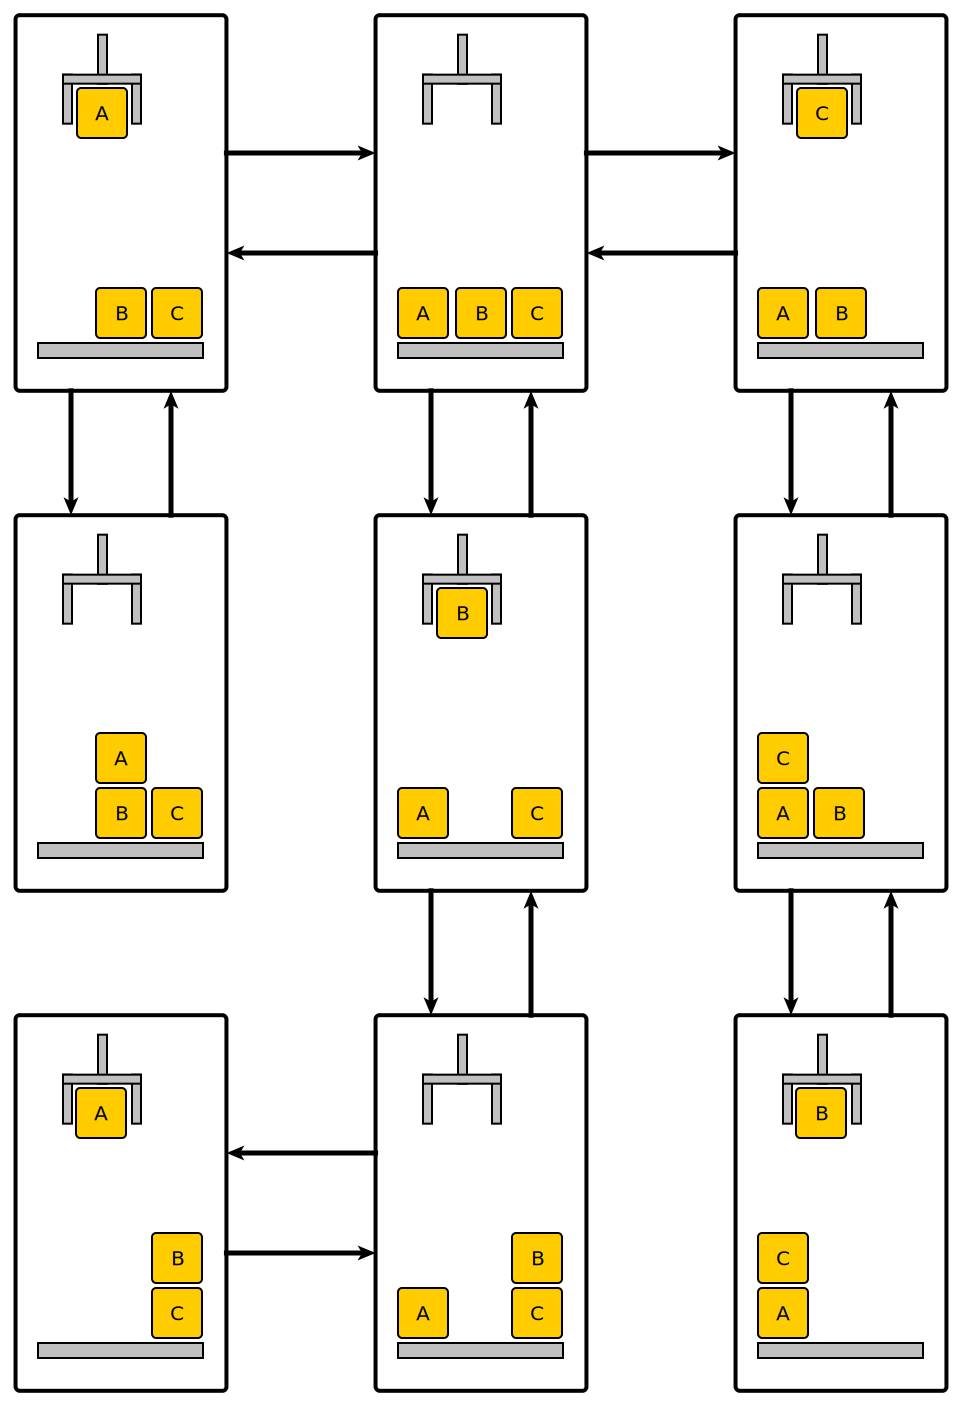
\includegraphics[scale=0.25]{./img/transicao_mundo_blocos.ps}
%	\caption[Exemplo de sistema de transi��o de estado no dom�nio do Mundo dos Blocos]{Exemplo de parte do sistema de %transi��o de estados no dom�nio do Mundo dos Blocos.}
%	\label{fig:sistemaTransicaoEstadoMundoBlocos}
%\end{figure}

\begin{figure}[ht!]
	\centering
	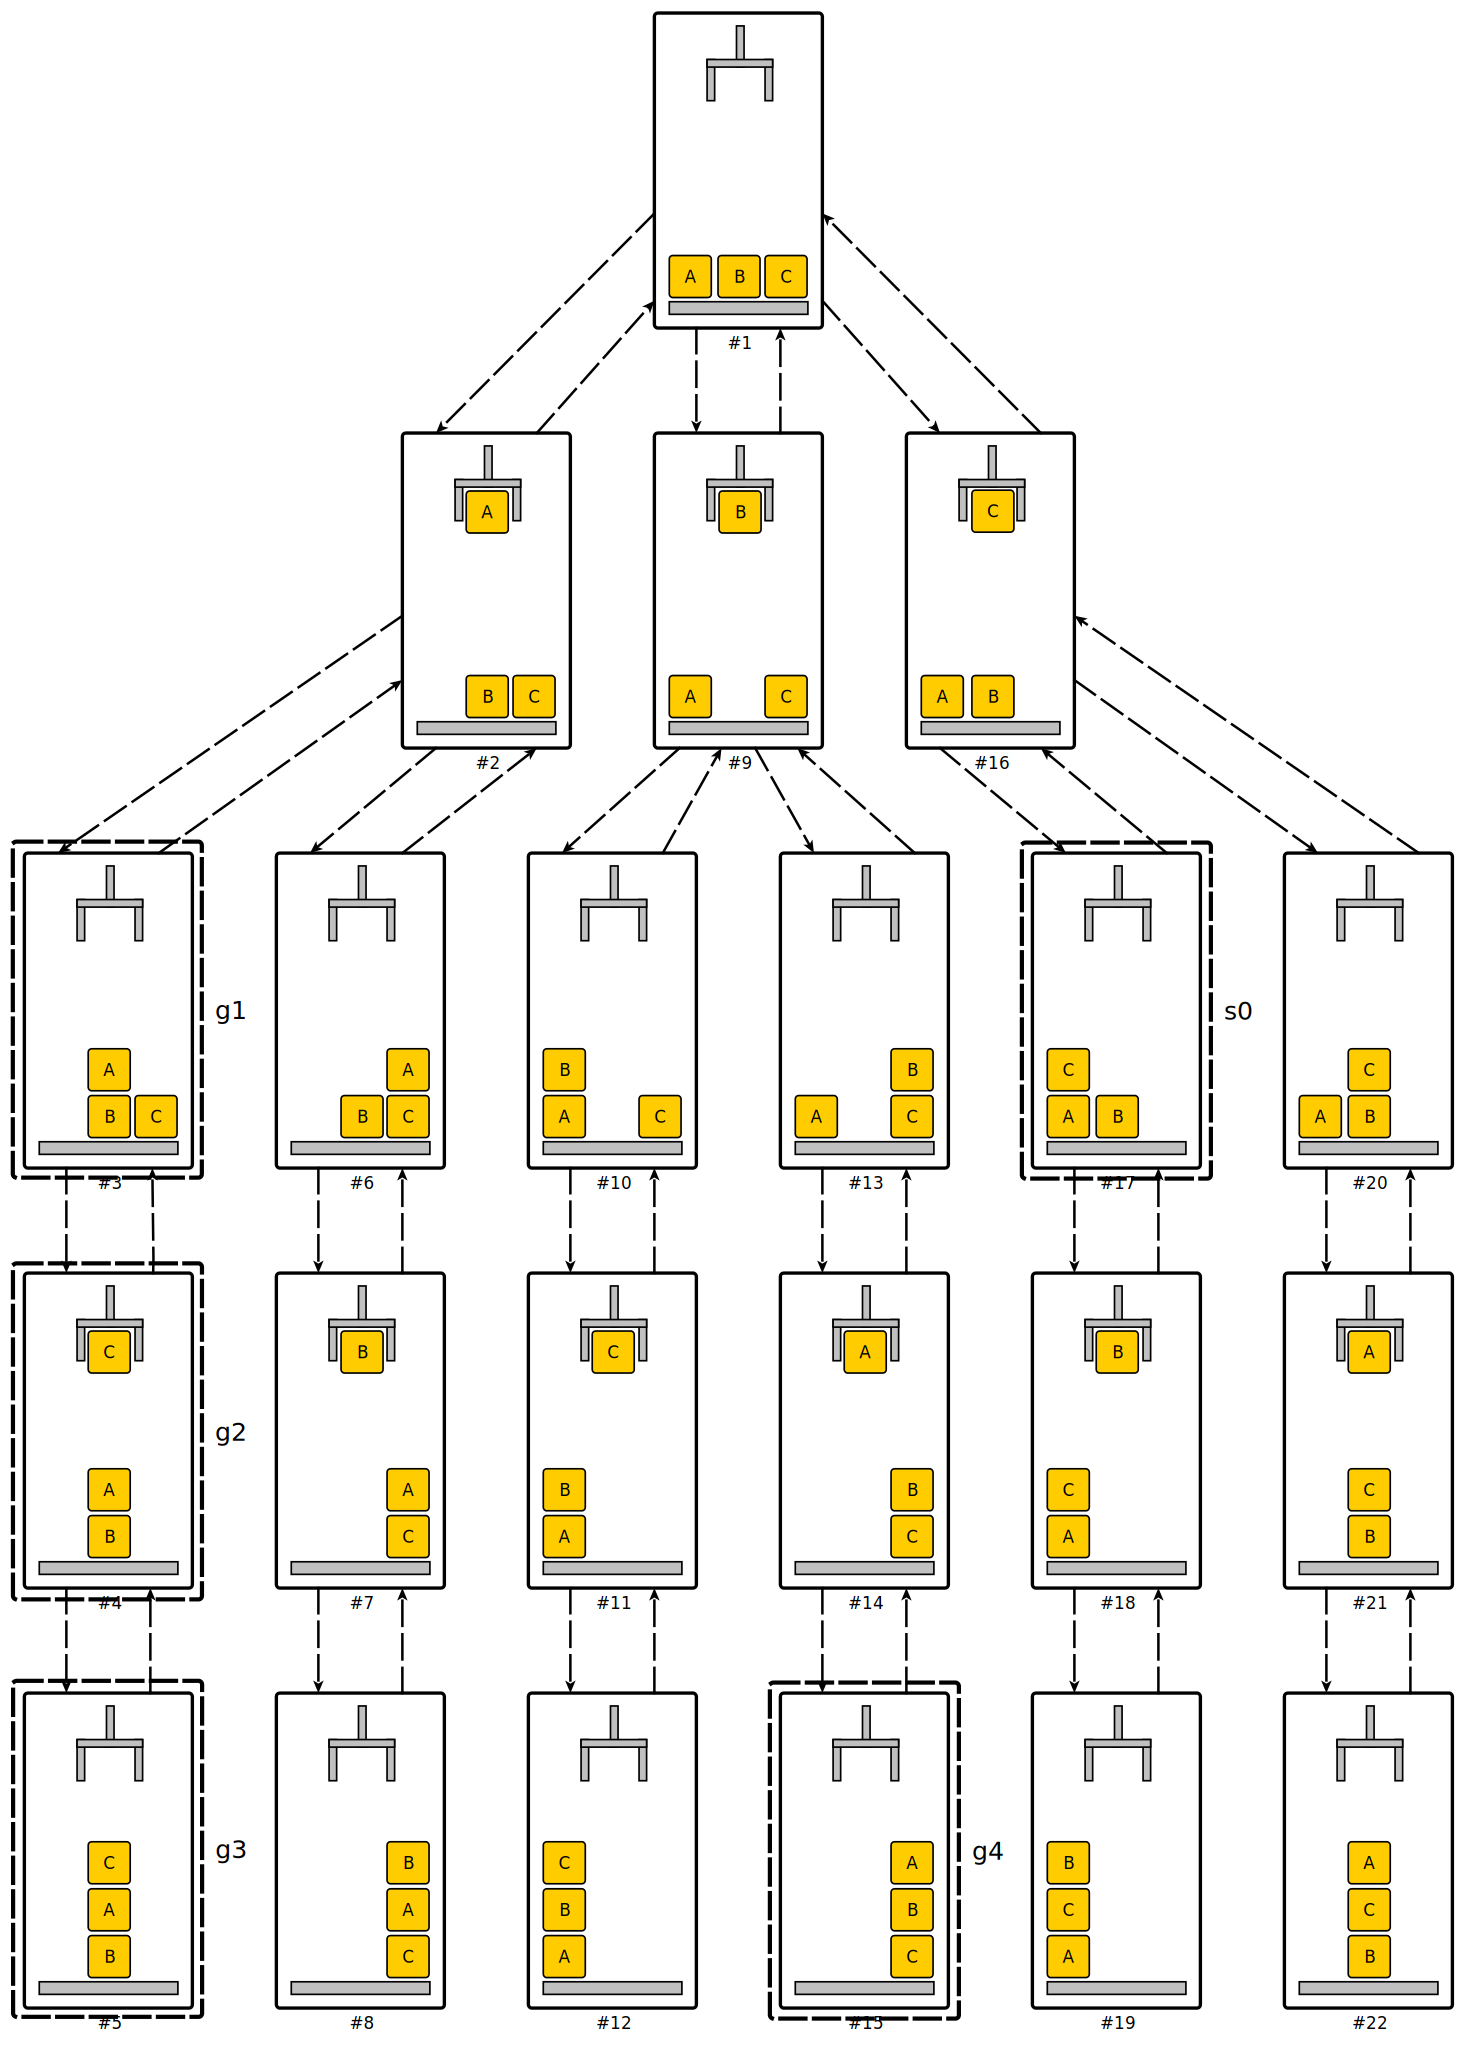
\includegraphics[scale=0.24]{./img/mundo_blocos_3_completo.ps}
	\caption[Sistema de transi��es de estados no dom�nio do Mundo dos Blocos]{Exemplo de sistema de transi��o de estados no dom�nio do Mundo dos Blocos\index{Mundo dos Blocos}. Nesta figura, os n�s representam todos os estados do mundo para um sistema com tr�s blocos e cada aresta representa uma transi��o de estado. Um exemplo de problema de planejamento seria encontrar um plano que a partir do estado $s_0$ conseguisse alcan�ar algum dos estados objetivos $\lbrace g_1,\ g_2,\ g_3,\ g_4 \rbrace$ \cite{Lago2002}.}
	\label{fig:sistemaTransicaoEstadoMundoBlocos}
\end{figure}

A propriedade sobre conhecimento completo � necess�ria somente no estado inicial $s_0$ porque o modelo determin�stico permite que todos os outros estados sejam completamente previs�veis, dado que as a��es s�o determin�sticas. Uma vez que a execu��o do plano � incondicional (sempre funciona), o controlador que executa o plano n�o obt�m nenhuma realimenta��o sobre o estado do sistema, como pode ser observado no modelo conceitual para planejamento visto no Cap�tulo \ref{cap:modelo_conceitual_planejamento}. \\

Este caso restrito pode parecer simples: planejamento se resume a buscar um caminho em um grafo\index{grafo}, sendo que este � um problema conhecido e bem resolvido. Na verdade, se for dado explicitamente o grafo $\Sigma$, ent�o n�o h� muito mais a dizer sobre planejamento para este caso. Entretanto, mesmo em um dom�nio simples, o grafo $\Sigma$ pode ser t�o extenso que especific�-lo explicitamente n�o � vi�vel. Al�m disso, este modelo foi proposto como uma base para futuras extens�es, como ser� visto no pr�ximo cap�tulo.\\

O {\it planejamento cl�ssico\index{planejamento!cl�ssico}} se refere genericamente a um planejamento para sistemas restritos de transi��es de estados. \\

\begin{Def}[Planejamento cl�ssico]
Um sistema restrito de transi��o de estados � aquele que satisfaz todas as suposi��es de A0 a A7. � um sistema de transi��o de estados determin�stico, est�tico, finito e completamente observ�vel com objetivos restritos e tempo impl�cito. Tal sistema � simbolizado por $\Sigma = (\mathcal{S}, \mathcal{A}, \gamma)$, e n�o por $(\mathcal{S},\ \mathcal{A},\ \mathcal{E},\ \gamma)$, porque n�o h� eventos ex�genos\index{evento!ex�geno}. Aqui, $\mathcal{S},\ \mathcal{A}$ e $\gamma$ s�o finitos, e $\gamma(s, a)$ � um estado �nico quando $a$ � aplic�vel em $s$ \cite{Malik2004}. \\
\end{Def}

\begin{Def}[Problema de planejamento cl�ssico]
Um problema de planejamento cl�ssico\index{planejamento!cl�ssico} para um sistema de transi��o de estado restrito\index{sistema!de transi��o de estado restrito} $\Sigma\ =\ (\mathcal{S},\ \mathcal{A},\ \gamma)$ � definido como uma tripla $\mathcal{P} = (\Sigma\ ,\ s_0,\ g)$, em que $s_0$ � um estado inicial e $g$ corresponde a um conjunto de estados objetivos. Uma solu��o para $\mathcal{P}$ � uma seq��ncia de a��es $(a_1,\ a_2,\ \ldots,\ a_k)$ correspondente a uma seq��ncia de transi��es de estados $(s_0,\ s_1,\ \ldots,\ s_k)$, tal que $s_1\ =\ \gamma(s_0,\ a_1),\ \ldots,\ s_k\ =\ \gamma(s_{k-1},\ a_k)$, onde $s_k$ � um estado objetivo. Tal seq��ncia de a��es deve ser sintetizada pelo sistema de planejamento.
\end{Def}

\section{Linguagens para planejamento}
\label{cap:3:sec:linguagens_para_planejamento}

No planejamento independente de dom�nio\index{planejamento!independente de dom�nio}, a representa��o de problemas de planejamento $-$ estados, a��es e objetivos $-$ deve ser feita por meio de uma linguagem que seja suficientemente expressiva para descrever uma ampla variedade de problemas, mas restritiva o bastante para permitir que algoritmos eficientes operem sobre ela. A maioria das abordagens de planejamento adotam uma representa��o baseada em l�gica\index{l�gica} para descrever estados, a��es e para definir e computar facilmente o pr�ximo estado $\gamma(s,a)$. A linguagem mais popular usada por planejadores cl�ssicos � conhecida como {STRIPS}\index{STRIPS} ({\it Stanford Research Institute Planning System}) \cite{Richard1971}, tem sido estendida nos �ltimos 15 anos para abranger problemas de planejamento n�o-cl�ssicos, isto �, planejamento para dom�nios mais complexos. Neste trabalho 

\subsection{Representa��o de estado}

A linguagem {STRIPS} decomp�e o mundo em condi��es l�gicas e representa um estado como uma conjun��o de literais positivos\index{literal!positivo}\footnote{Em l�gica de predicados de primeira ordem\index{l�gica!de predicados de primeira ordem}\index{l�gica!proposicional}, um {\it literal}\index{literal} � uma senten�a at�mica (um {\it literal positivo}\index{literal!positivo}) ou uma senten�a at�mica negada (um {\it literal negativo}\index{literal!negativo}).}. Um exemplo de literal proposicional que pode representar o estado de um agente desaparecido �  $Perdido\ \wedge\ Incomunicavel$. J� literais de primeira ordem podem ser representados por $Cor(Bloco_1,\ Azul)\ \wedge\ Cor(Bloco_2,\ Vermelho)\ \wedge\ Sobre(Bloco_1,\ Bloco_2)$. Literais utilizados em descri��es de estado de primeira ordem devem ser b�sicos e livres de fun��es. Al�m disso, numa representa��o de estado, quaisquer condi��es n�o mencionadas em um estado s�o consideradas falsas, esta premissa � conhecida como \ac{CWA}\index{mundo!fechado}. \\

\subsection{Representa��o de objetivo}

Um objetivo na linguagem {STRIPS}\index{STRIPS} � dado por uma conjun��o de literais b�sicos positivos. Por exemplo, pode-se representar o objetivo de ter um bolo e estar com a cozinha limpa por meio de $Bolo\ \wedge\ CozinhaLimpa$ ou que o $Bloco_2$ deve estar sobre o $Bloco_1$ por $Sobre(Bloco_2,\ Bloco_1)$. Um estado $s$ {\it satisfaz\index{satisfaz}} um objetivo $g$ se $s$ cont�m todos os literais (ou proposi��es) em $g$. Por exemplo, o estado $Bolo\ \wedge\ CozinhaLimpa\ \wedge\ Suco$ satisfaz o objetivo $Bolo\ \wedge\ CozinhaLimpa$.

\subsection{Representa��o de a��es}

Uma a��o {STRIPS} � descrita pelas pr�-condi��es (literais positivos) que devem ser v�lidas antes de a mesma ser aplicada e pelos efeitos ap�s sua execu��o. Por exemplo, a composi��o da representa��o de uma a��o equivalente a dirigir um carro de um local para outro pode ser observada na Tabela 3.2. \\

\begin{Tab}[Exemplo de representa��o de uma a��o STRIPS]
\ \\
\begin{tabular}{|l|l|}
\hline
A��o          &  \scriptsize Dirigir($carro$, $origem$, $destino$)\\
Pr�-condi��es &  \scriptsize Em($carro$, $origem$) $\wedge$ Ve�culo($carro$) $\wedge$ Cidade($origem$) $\wedge$ Cidade($destino$)\\
Efeitos       &  \scriptsize $\lnot$ Em($carro$, $origem$) $\wedge$ Em($carro$, $destino$)\\
\hline
\end{tabular}
\end{Tab}

A estrutura de uma a��o {STRIPS} no planejamento cl�ssico consiste de tr�s partes:

\begin{itemize}

\item O \textbf{nome da a��o} e a lista de par�metros. Por exemplo, {\it Dirigir}({\it carro,\ origem,\ destino}) serve para identificar a a��o.

\item A \textbf{pr�-condi��o} � uma conjun��o de literais positivos que devem ser verdadeiros em um estado antes da a��o ser executada. Qualquer vari�vel da pr�-condi��o tamb�m deve aparecer na lista de par�metros da a��o.

\item Os \textbf{efeitos} da a��o s�o representados por uma conjun��o de literais livres de fun��es que descrevem como o estado se altera quando a a��o � executada. Um literal positivo ($p$) no efeito � considerado verdadeiro no estado resultante da a��o, enquanto que sua nega��o ($\lnot p$) significa que ele � falso naquele estado. As vari�veis do efeito tamb�m devem aparecer na lista de par�metros da a��o.

\end{itemize}

Deste modo, uma a��o � {\it aplic�vel\index{a��o!aplic�vel}} a qualquer estado que satisfa�a a pr�\-con\-di\-��o; caso contr�rio, a a��o n�o tem nenhum efeito. O resultado da execu��o de uma a��o aplic�vel $a$ em um estado $s$ � $s'$, o qual � calculado eliminando-se os literais negativos e adicionando-se os literais positivos dos efeitos de $a$. Assim, se um efeito positivo j� estiver em $s$, ele n�o ser� adicionado uma segunda vez, e se um efeito negativo n�o estiver em $s$, o mesmo ser� ignorado. Qualquer literal n�o mencionado no efeito permanece inalterado. \\

\subsection{Dom�nio do Mundo dos Blocos}
\label{cap:3:sec:linguagens_para_planejamento:subsub:mundo_de_blocos}

O Mundo dos Blocos\index{Mundo dos Blocos} � um dos dom�nios de planejamento mais famosos \cite{Winston1992}. Este dom�nio consiste em um conjunto de blocos em forma de cubo, dispostos sobre uma mesa. Os blocos podem ser empilhados, mas apenas um bloco pode ficar diretamente em cima de outro. Um bra�o rob�\index{rob�} pode levantar um bloco de cada vez, por�m n�o consegue levantar um bloco que tenha outro em cima dele. O objetivo � construir uma ou mais pilhas de blocos, com especifica��es exatas de quais blocos devem ficar em cima de que outros blocos. Por exemplo, um objetivo poderia ser colocar o bloco {\it A} sobre {\it B} e o bloco {\it B} sobre {\it C}. Um exemplo deste dom�nio pode ser visto na Figura 3.2, e sua descri��o encontra-se no Ap�ndice \ref{apendice_dominio_blocos}. \\

\begin{figure}[ht!]
    \centering
	\label{fig:mundo_blocos}
    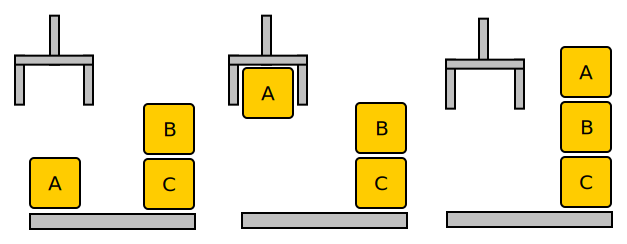
\includegraphics[angle=0,width=1.0\textwidth]{./img/mundo_blocos.ps}
    \caption[Mundo dos Blocos]{Este exemplo demonstra o comportamento de a��es comuns no Mundo dos Blocos\index{Mundo dos Blocos}, ao empilhar o bloco A sobre o bloco B.}
\end{figure}

A Tabela 3.1 mostra a descri��o de todos os estados, em {STRIPS}, apresentados na Figura 3.1.

\begin{Tab}[Todos os estados do dom�nio do Mundo dos Blocos para um problema com 3 blocos]
\ \\
\begin{tabular}{|c|l|}
\hline
Estado & Descri��o \\
\hline
$\#1$ & \scriptsize GarraVazia $\wedge$ Sobre(A, Mesa) $\wedge$ Sobre(B, Mesa) $\wedge$ Sobre(C, Mesa) $\wedge$ 
\\ & \scriptsize Livre(A) $\wedge$ Livre(B) $\wedge$ Livre(C) \\

$\#2$ & \scriptsize Garra(A) $\wedge$ Sobre(B, Mesa) $\wedge$ Sobre(C, Mesa) $\wedge$ Livre(B) $\wedge$ Livre(C) \\

$\#3$ &  \scriptsize GarraVazia $\wedge$ Sobre(A, B) $\wedge$ Sobre(B, Mesa) $\wedge$ Sobre(C, Mesa) $\wedge$ Livre(A) $\wedge$ Livre(C) \\
$\#4$ &  \scriptsize Garra(C) $\wedge$ Sobre(A, B) $\wedge$ Sobre(B, Mesa) $\wedge$ Livre(A) \\
$\#5$ &  \scriptsize GarraVazia $\wedge$ Sobre(A, B) $\wedge$ Sobre(B, Mesa) $\wedge$ $\wedge$ Sobre(C, A) $\wedge$ Livre(C) \\

$\#6$ &  \scriptsize GarraVazia $\wedge$ Sobre(A, C) $\wedge$ Sobre(B, Mesa) $\wedge$ Sobre(C, Mesa) $\wedge$ Livre(A) $\wedge$ Livre(B) \\
$\#7$ &  \scriptsize Garra(B) $\wedge$ Sobre(A, C) $\wedge$ Sobre(C, Mesa) $\wedge$ Livre(A) \\
$\#8$ &  \scriptsize GarraVazia $\wedge$ Sobre(A, C) $\wedge$ Sobre(B, A) $\wedge$ Sobre(C, Mesa) $\wedge$ Livre(C) \\

$\#9$ & \scriptsize Garra(B) $\wedge$ Sobre(A, Mesa) $\wedge$ Sobre(C, Mesa) $\wedge$ Livre(A) $\wedge$ Livre(C) \\

$\#10$ & \scriptsize GarraVazia $\wedge$ Sobre(A, Mesa) $\wedge$ Sobre(B, A) $\wedge$ Sobre(C, Mesa) $\wedge$ Livre(B) $\wedge$ Livre(C) \\
$\#11$ & \scriptsize Garra(C) $\wedge$ Sobre(A, Mesa) $\wedge$ Sobre(B, A) $\wedge$ Livre(B) \\
$\#12$ & \scriptsize GarraVazia $\wedge$ Sobre(A, Mesa) $\wedge$ Sobre(B, A) $\wedge$ Sobre(C, B) $\wedge$ Livre(C) \\

$\#13$ & \scriptsize GarraVazia $\wedge$ Sobre(A, Mesa) $\wedge$ Sobre(B, C) $\wedge$ Sobre(C, Mesa) $\wedge$ Livre(A) $\wedge$ Livre(B) \\
$\#14$ & \scriptsize Garra(A) $\wedge$ Sobre(B, C) $\wedge$ Sobre(C, Mesa) $\wedge$ Livre(B) \\
$\#15$ & \scriptsize GarraVazia $\wedge$ Sobre(A, B) $\wedge$ Sobre(B, C) $\wedge$ Sobre(C, Mesa) $\wedge$ Livre(A) \\

$\#16$ & \scriptsize Garra(C) $\wedge$ Sobre(A, Mesa) $\wedge$ Sobre(B, Mesa) $\wedge$ Livre(A) $\wedge$ Livre(B) \\

$\#17$ & \scriptsize GarraVazia $\wedge$ Sobre(A, Mesa) $\wedge$ Sobre(B, Mesa) $\wedge$ Sobre(C, A) $\wedge$ Livre(B) $\wedge$ Livre(C) \\
$\#18$ & \scriptsize Garra(B) $\wedge$ Sobre(A, Mesa) $\wedge$ Sobre(C, A) $\wedge$ Livre(C) \\
$\#19$ & \scriptsize GarraVazia $\wedge$ Sobre(A, Mesa) $\wedge$ Sobre(B, C) $\wedge$ Sobre(C, A) $\wedge$ Livre(B) \\

$\#20$ & \scriptsize GarraVazia $\wedge$ Sobre(A, Mesa) $\wedge$ Sobre(B, Mesa) $\wedge$ Sobre(C, B) $\wedge$ Livre(A) $\wedge$ Livre(C) \\
$\#21$ & \scriptsize Garra(A) $\wedge$ Sobre(B, Mesa) $\wedge$ Sobre(C, B) $\wedge$ Livre(C) \\
$\#22$ & \scriptsize GarraVazia $\wedge$ Sobre(A, C) $\wedge$ Sobre(B, Mesa) $\wedge$ Sobre(C, B) $\wedge$ Livre(A) \\
\hline
\end{tabular}
\\
\end{Tab}

Na Tabela 3.3 � poss�vel observar as a��es {STRIPS} para o dom�nio do Mundo dos Blocos.

\begin{Tab}[A��es STRIPS para o dom�nio do Mundo dos Blocos]
\ \\
\begin{tabular}{|l|l|}
\hline
A��o          &  \scriptsize PegarMesa($bloco$)\\
Pr�-condi��es &  \scriptsize GarraVazia $\wedge$ Sobre($bloco$, Mesa) $\wedge$ Livre($bloco$) \\
Efeitos       &  \scriptsize $\lnot$ GarraVazia\ $\wedge$\ Garra($bloco$) $\wedge$ $\lnot$ Sobre($bloco$, Mesa) $\wedge$ $\lnot$ Livre(bloco) \\
\hline
A��o          &  \scriptsize ColocarMesa($bloco$) \\
Pr�-condi��es &  \scriptsize Garra($bloco$) \\
Efeitos       &  \scriptsize GarraVazia\ $\wedge$\ $\lnot$ Garra($bloco$) $\wedge$ Sobre($bloco$, Mesa) $\wedge$ Livre($bloco$) \\
\hline
A��o          &  \scriptsize Desempilhar($bloco_1$, $bloco_2$) \\
Pr�-condi��es &  \scriptsize GarraVazia $\wedge$ Sobre($bloco_1$, $bloco_2$) $\wedge$ Livre($bloco_1$) \\
Efeitos       &  \scriptsize $\lnot$ GarraVazia\ $\wedge$\ Garra($bloco_1$) $\wedge$ $\lnot$ Sobre($bloco_1$, $bloco_2$) $\wedge$
\\ & \scriptsize $\lnot$ Livre($bloco_1$) $\wedge$ Livre($bloco_2$) \\
\hline
A��o          &  \scriptsize Empilhar($bloco_1$, $bloco_2$) \\
Pr�-condi��es &  \scriptsize Garra($bloco_1$) $\wedge$ Livre($bloco_2$) \\
Efeitos       &  \scriptsize GarraVazia\ $\wedge$\ $\lnot$ Garra($bloco_1$) $\wedge$ Sobre($bloco_1$, $bloco_2$) $\wedge$
\\ & \scriptsize Livre($bloco_1$) $\wedge$ $\lnot$ Livre($bloco_2$) \\
\hline
\end{tabular}
\end{Tab}

\subsection{Linguagens para dom�nios reais}

Com as defini��es dadas da linguagem {STRIPS}\index{STRIPS} � poss�vel definir uma {\it solu��o\index{solu��o}} para planejamento como uma seq��ncia de a��es que, quando executadas, resultam em um estado que satisfaz o objetivo. \\

Para dom�nios reais\index{dom�nio!real}\index{mundo!real}, a linguagem {STRIPS} n�o � considerada uma linguagem expressiva o suficiente. Devido a isso, foram desenvolvidas muitas variantes de linguagem, sendo uma delas a \ac{ADL}\index{ADL} \cite{Pednault1989}. Em {STRIPS} s� � permitido o uso de literais positivos\index{literal!positivo} em estados, enquanto em \ac{ADL} s�o permitidos literais positivos e negativos\index{literal!negativo}. {STRIPS} trabalha com a {\it suposi��o de mundo fechado}\index{suposi��o!de mundo fechado}, em que literais n�o mencionados s�o falsos. Em contrapartida, a \ac{ADL} trabalha com a {\it suposi��o de mundo aberto}\index{hip�tese!de mundo aberto}, em que literais n�o mencionados s�o desconhecidos. Uma outra diferen�a importante � que em {STRIPS} n�o h� fun��es como para igualdade, e n�o � poss�vel definir tipos de dados; j� \ac{ADL} apresenta tais caracter�sticas, bem como quantificadores sobre objetos do dom�nio. \\

As diversas formas de planejamento em {IA}\index{IA} podem ser especificadas por meio de uma sintaxe padr�o denominada {PDDL}\index{PDDL} ({\it Problem Domain Definition Language}) \cite{McDermott1998}\cite{McDermott1998a}, que inclui, entre outras, a linguagem {STRIPS} e \ac{ADL}. Mais informa��es sobre {PDDL} podem ser encontradas no Ap�ndice \ref{apendice_pddl}. \\

\section{Algoritmos tradicionais para planejamento cl�ssico}

\subsection{Busca no espa�o de estados}

A busca no espa�o de estados\index{busca!espa�o de estados} � empregada por v�rios algoritmos de planejamento. O espa�o de estados pode ser representado por um grafo\index{grafo}, em que cada n� corresponde a um estado do mundo e cada aresta a uma transi��o de estado. O planejamento no espa�o de estados divide-se basicamente em algoritmos {\it progressivos\index{algoritmo!progressivo}} e {\it regressivos\index{algoritmo!regressivo}}. \\

O algoritmo progressivo de busca parte do estado inicial do plano e aplica de forma n�o-determin�stica, a fun��o de transi��o de estado, isto �, todas as seq��ncias de a��es poss�veis, produzindo outros estados e, conseq�entemente, subproblemas. Estes subproblemas buscam solu��es parciais que levam ao estado desejado, pois s�o parte do problema original. A busca � finalizada quando um destes subproblemas consegue alcan�ar um estado objetivo ou quando n�o h� nenhum plano poss�vel, caracterizando assim uma falha. \\

Uma das caracter�sticas do planejamento progressivo � o de ter conhecimento completo sobre o estado do mundo a
qualquer instante. Isto se deve ao fato de que este opera a partir de um estado inicial completamente especificado e aplica a��es aos estados, resultando em mais especifica��es completas. O Algoritmo \ref{algoritmo_planejamento_progressivo} exemplifica o processo de planejamento progressivo. \\

\begin{algorithm}
	\label{algoritmo_planejamento_progressivo}
	\caption[Planejamento progressivo]{Planejamento progressivo.}
	\Entrada{Estado inicial $s_0$, Objetivo $S_g$, Dom�nio $\mathcal{D}$}
	\Saida{Plano $\pi$}
	\Inicio{
		$\pi \leftarrow 0$\;
		$s \leftarrow s_0$\;
		\Repita{}{
			\Se{$s\ \in\ S_g$}{
				{\bf devolve} $\pi$\;
			}
			$A \leftarrow \lbrace a \mid a$ � uma a��o aplic�vel a $s \rbrace$\;
			\Se{$A = 0$}{
				{\bf devolve} $falha$\;
			}
			n�o-deterministicamente escolha $a \in A$\;
			$\pi \leftarrow \pi + a$\;
			$s \leftarrow \gamma(s,\ a)$\;	
		}
	}
\end{algorithm}

Tamb�m � poss�vel efetuar planejamento no espa�o de estados\index{planejamento!espa�o de estados} por meio de uma busca regressiva. Neste processo o procedimento � o inverso da busca progressiva, come�ando pela aplica��o da fun��o de transi��o inversa ao estado objetivo. Com isso s�o produzidos estados predecessores, nos quais a fun��o de transi��o � aplicada novamente e assim sucessivamente at� que chegue ao estado incial. As representa��es que seguem o modelo {STRIPS} tornam esta descri��o bastante f�cil, porque os conjuntos de estados podem ser descritos pelos literais que devem ser verdadeiros em tais estados (isto �, as pr�-condi��es das a��es). \\

Desde o in�cio das pesquisas, na d�cada de 60, com o \ac{GPS}\index{GPS} \cite{Newell1961}, os algoritmos de busca progressiva s�o utilizados, sendo especializados com heur�sticas $A^*$\index{$A^*$} \cite{Hart1968} e, hoje, correspondem aos melhores planejadores para o modelo restrito (planejamento cl�ssico).\\

\subsection{Busca no espa�o de planos}

{\it Planejamento no espa�o de planos\index{planejamento!espa�o de planos}} � um outro meio de encontrar solu��es para problemas de planejamento cl�ssico \cite{Malik2004}. A busca progressiva e regressiva no espa�o de estados s�o formas espec�ficas de busca de planos {\it totalmente ordenados}. Elas exploram apenas seq��ncias estritamente lineares de a��es conectadas de forma direta ao estado inicial ou ao objetivo, ou seja n�o podem se beneficiar da decomposi��o do problema. Ao inv�s de atuarem sobre cada subproblema separadamente, elas sempre t�m de tomar decis�es a respeito de como definir seq��ncias de a��es a partir de todos os subproblemas \cite{Russell2002}. \\

Por outro lado, uma abordagem que apresenta v�rios sub-objetivos independentes demonstra uma vantagem de flexibilidade na ordem de elabora��o do plano. O planejador pode trabalhar primeiro em decis�es �bvias ou importantes, onde somente algumas a��es s�o ordenadas com rela��o �s demais (compromissos fracos), em vez de ser for�ado a atuar em etapas dispostas em ordem cronol�gica em rela��o �s a��es (compromissos fortes). \\

Deste modo, qualquer algoritmo de planejamento que possa inserir duas a��es em um plano sem especificar qual delas deve ser executada primeiro � definido como {\it planejamento de ordem parcial\index{planejamento!ordem parcial}}. O planejador de ordem parcial pode ser implementado sob a forma de uma busca no espa�o de planos de ordem parcial (em alguns momentos chamados apenas de planos parciais). \\

O processo se inicia com um plano vazio, em seguida, s�o considerados meios de aprimorar o plano at� que se obtenha um plano completo que resolva o problema. As a��es nesta busca n�o s�o a��es no mundo, mas a��es sobre planos: adicionar um passo ao plano, impor uma ordena��o que coloque uma a��o antes de outra e, assim sucessivamente. Os n�s do espa�o de busca s�o planos e, em sua maioria, n�o conclu�dos, isto �, planos parciais. Cada plano possui quatro componentes, sendo que os dois primeiros definem os passos do plano e os dois �ltimos determinam como os planos podem ser estendidos. Os componentes do plano s�o descritos a seguir:

\begin{itemize}
\item \textbf{Um conjunto de a��es que comp�em os passos do plano}. Estas a��es s�o obtidas do conjunto de todas as a��es poss�veis para o problema de planejamento,sendo que um plano {\it vazio} cont�m apenas as a��es {\it Iniciar} e {\it Terminar}. {\it Iniciar} n�o tem pr�-condi��es e apresenta como efeito todos os literais no estado inicial do problema de planejamento. {\it Terminar} n�o tem efeitos e tem como pr�-condi��es os literais de objetivo do problema de planejamento. \\

\item \textbf{Um conjunto de restri��es de ordena��o}. Cada restri��o de ordena��o tem a forma $A \prec B$, isto significa que a a��o $A$ deve ser executado antes de $B$, mas n�o imediatamente antes. \\

\item \textbf{Um conjunto de v�nculos causais}. Um v�nculo causal\index{v�nculo causal} entre as a��es $A$ e $B$ no plano � escrito como $A \stackrel{p}{\rightarrow} B$. Isto afirma que $p$ � um efeito da a��o $A$ e uma pr�-condi��o de $B$, e tamb�m significa que $p$ dever� permanecer verdadeiro entre as a��es $A$ e $B$. A a��o $A$ � chamada de a��o que contribui com $p$, e $B$ a a��o que necessita de $p$. Deste modo, o plano n�o pode ser estendido adicionando-se uma nova a��o $C$ que esteja em conflito com o v�nculo causal. A a��o $C$ est� em conflito com $A \stackrel{p}{\rightarrow} B$, se $C$ tem efeito $\lnot p$ e se $C$ pode ocorrer depois de $A$ e antes de $B$. V�nculos causais tamb�m podem ser chamados de {\it intervalos de prote��o\index{intervalos de prote��o}}. \\

\item \textbf{Um conjunto de pr�-condi��es abertas}. Uma pr�-condi��o � aberta\index{pr�-condi��o!aberta} se n�o � alcan�ada por alguma a��o do plano. Os planejadores trabalham para reduzir o conjunto de pr�-condi��es abertas a um conjunto vazio, sem introduzir conflitos.
\end{itemize}

Um {\it plano consistente\index{plano!consistente}} � aquele que n�o possui ciclo nas restri��es de ordena��o e nenhum conflito com os v�nculos causais. Deste modo, um plano consistente sem pr�-condi��es abertas � uma solu��o. Um exemplo de plano de ordem parcial e suas lineariza��es correspondentes em planos de ordem total pode ser visto na Figura 3.3.
%TODO: 

\begin{figure}[ht!]
	\centering
	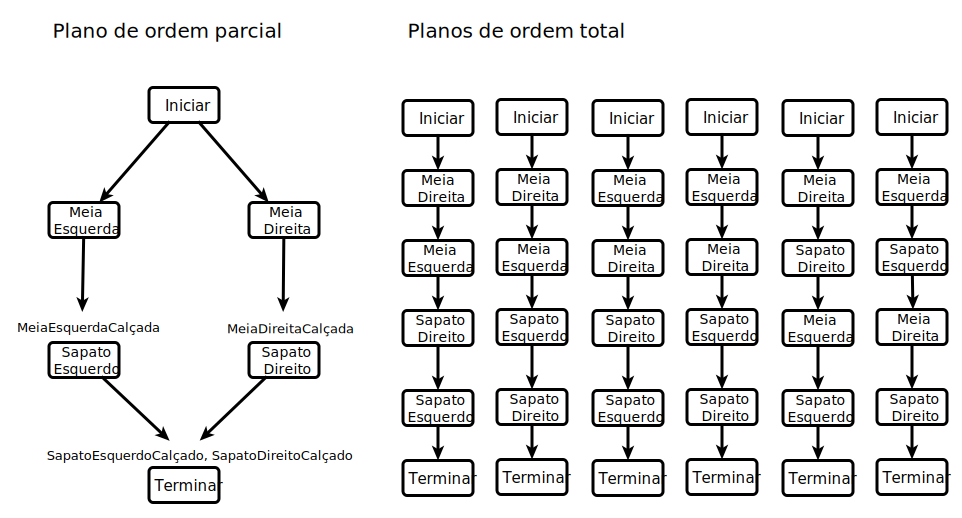
\includegraphics[angle=270,scale=0.75,width=1.0\textwidth]{./img/plano_ordem_parcial.ps} 
	\label{fig:plano_ordem_parcial}
	\caption[Plano de ordem parcial e suas lineariza��es]{Exemplo de um plano de ordem parcial para cal�ar sapatos e meias, e as seis lineariza��es correspondentes em planos de ordem total \cite{Russell2002}. A solu��o � apresentada em um grafo\index{grafo!de a��es} de a��es no qual � poss�vel observar as a��es Iniciar e Terminar, que marcam o in�cio e o final do plano. A solu��o de ordem parcial\index{ordem!parcial} corresponde a seis planos poss�veis de ordem total\index{plano!de ordem total}\index{ordem!total}; cada um desses planos � uma lineariza��o\index{lineariza��o} do plano de ordem parcial\index{plano!de ordem parcial}.}
\end{figure}

Um algoritmo cl�ssico de planejamento como busca no espa�o de planos, completamente provado e correto, � o \ac{POP} \cite{Russell2002}.\\

\section{Planejamento por refinamento}

A constru��o de um plano pode ser vista como um refinamento\index{refinamento} iterativo do conjunto de todos os planos poss�veis. Esta estrat�gia � chamada de {\it planejamento por refinamento\index{planejamento!por refinamento}} (\cite{Kambhampati1997}). � poss�vel demonstrar que a maioria dos algoritmos cl�ssicos de planejamento pode ser compreendida desta maneira (incluindo o \ac{POP}). A id�ia principal do planejamento por refinamento � que, iniciando com um conjunto de todas as seq��ncias poss�veis de a��es do dom�nio (a��es {STRIPS}), num processo iterativo, adicionam-se restri��es\index{restri��es} de modo a reduzir este espa�o de planos\index{espa�o de plano}. As restri��es podem impor ordem entre as a��es ou que uma proposi��o particular deva ser verdade em um ponto espec�fico do plano. Cada etapa (ou passo) do plano � identificada por um elemento �nico e corresponde a uma a��o. A seguir, s�o descritos os tipos b�sicos de restri��es no planejamento por refinamento: \\

{\bf Restri��es de ordem}\index{restri��o!de ordem} \\

\begin{itemize}
\item \textit{Restri��o de preced�ncia}\index{restri��o!de preced�ncia}. Um passo precede outro passo do plano, sendo que outros passos podem ocorrer entre eles.
\item \textit{Restri��o de contig�idade}\index{restri��o!de contig�idade}. Um passo deve preceder imediatamente um outro passo, isto �, nenhum outro passo deve ocorrer entre eles.
\end{itemize}
 
{\bf Restri��es auxiliares}\index{restri��o!auxiliar} \\

\begin{itemize}

\item \textit{Restri��o de prote��o de intervalo}\index{restri��o!prote��o de intervalo} \textit{ou de v�nculo causal}\index{v�nculo causal}. Essa restri��o imp�e que uma condi��o deve permanecer verdadeira sobre um intervalo (nenhuma a��o que tem efeito $p$ ser� permitida em um intervalo em que a condi��o $\lnot p$ deva ser preservada).

\item \textit{Restri��o de verdade pontual}\index{restri��o!verdade pontual}. A verdade de uma condi��o em um ponto particular do tempo deve ser preservada.

\end{itemize}

Neste tipo de planejamento, o processo de adi��o de restri��es continua at� que todos os planos que satisfa�am as restri��es sejam solu��es para o problema. Durante este refinamento n�o � armazenado o conjunto de todos os planos {\it candidatos}\index{plano!candidato}, mas apenas as restri��es. Estas restri��es s�o armazenadas em um {\it plano parcial\index{plano!parcial}}, sendo que, neste caso, um plano parcial $\mathcal{P}$ representa um conjunto de planos candidatos, que ser� chamado de {\it candidatos($\mathcal{P}$)}. \\

Uma estrat�gia de {\it refinamento} define como um plano parcial deve ser estendido por meio da adi��o de novas restri��es, sendo que tal adi��o ser� respons�vel pelo refinamento do conjunto de planos candidatos. Uma estrat�gia de refinamento $\mathcal{R}$ � uma fun��o que mapeia um plano parcial $\mathcal{P}$ em um conjunto de planos parciais, isto �, $\mathcal{P}\ =\ {\mathcal{P}_1,\ \ldots\ ,\mathcal{P}_i,\ \ldots\ ,\mathcal{P}_n}$, de forma que, para cada um dos planos parciais $\mathcal{P}_i$, o conjunto de candidatos ($\mathcal{P}_i$) seja um subconjunto de $candidatos(\mathcal{P})$. A Figura 3.4
%TODO: ~\ref{fig:conceito_refinamento} 
ilustra a defini��o geral de um planejador por refinamento. \\

\begin{figure}[ht!]
	\centering
	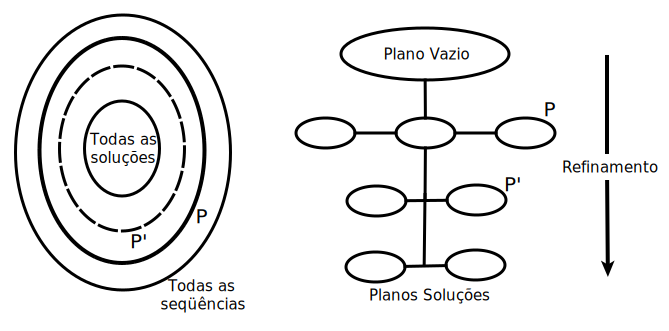
\includegraphics[angle=0,width=1.0\textwidth]{./img/visao_planejamento_refinamento.ps} 
	\label{fig:conceito_refinamento}
	\caption[Vis�o geral de planejamento por refinamento]{Vis�o geral de
	planejamento por refinamento \cite{Kambhampati1997}.}
\end{figure}

A partir de um conjunto vazio de restri��es, representado por um plano parcial vazio $\mathcal{P}$; � poss�vel verificar se um dos candidatos de $\mathcal{P}$ � uma solu��o do problema. Se for, finaliza-se o processo; caso contr�rio, aplica-se novamente uma estrat�gia de refinamento\index{estrat�gia de refinamento} $\mathcal{R}$ para obter uma cole��o de planos parciais $\mathcal{P'}\ =\ \mathcal{R}(\mathcal{P})$, em que cada plano parcial $\mathcal{P}_i$ possui uma restri��o adicional em rela��o a $\mathcal{P}$. Isto � feito selecionando-se um plano candidato de $\mathcal{P'}$ e verificando novamente se ele � uma solu��o; caso n�o seja, aplica-se novamente $\mathcal{R}$. Este processo deve continuar at� que se obtenha uma solu��o ou at� que o conjunto de planos parciais esteja vazio e, neste caso, � necess�rio retroceder. O Algoritmo ~\ref{algoritmo_planejamento_refinamento} realiza o processo de planejamento por refinamento.\\

\begin{algorithm}
	\label{algoritmo_planejamento_refinamento}
	\caption[Planejamento por refinamento]{Planejamento por refinamento}
	% \Entrada{Plano parcial $\mathcal{P}$, Problema $\Pi$, Hist�rico $\mathcal(H)$}
	\Entrada{Plano parcial $\mathcal{P}$, Problema $\Pi$}
	\Saida{Solu��o para $\Pi$ ou {\it falha}}
	\Inicio{
	    \Se{$candidatos(\mathcal{P}) = \emptyset$}{{\bf devolve} {\it falha}\;}
	    \Se{existe $solucao(\mathcal{P}, \Pi)$}
	    	    {{\bf devolve} $solucao(\mathcal{P}, \Pi)$\;}
            Selecionar estrat�gia de refinamento $\mathcal{R}$\;
	    Gerar novo conjunto de planos
	    %$\left<\mathcal{P, H'}\right> = \mathcal{R}(\mathcal{P, H})$\;
	    $\left<\mathcal{P, H'}\right> = \mathcal{R}(\mathcal{P})$\;
	    \Para{todo $\mathcal{P}_i \in \mathcal{P}$ escolhido n�o-deterministicamente} {
		    \textsc{Planejamento Por Refinamento} ($\mathcal{P}_i, \Pi, \mathcal{H'}$)\;
		}
	}
\end{algorithm}

\subsection{VHPOP}

Um dos planejadores que implementa de forma expl�cita o planejamento por refinamento � o \ac{VHPOP}. \\

O \ac{VHPOP}\index{VHPOP} � um planejador de ordem parcial ({\it Partial Order Causal Link} - POCL) baseado no {UCPOP}\index{UCPOP} ({\it Partial Order Planner with Conditional effects and Universal quantification}) \cite{DBLP:conf/kr/PenberthyW92}. O \ac{VHPOP} � resultado de experi�ncias obtidas em meados dos anos 90 no estudo de estrat�gias para planejamento {POCL}\index{POCL}, combinado com avan�os no campo do planejamento independente de dom�nio, como an�lise de alcan�abilidade \cite{Younes2003}. \\

Ao incorparar t�cnicas para restri��es temporais, o \ac{VHPOP}\index{VHPOP} assume a capacidade de fazer planejamento utilizando a��es com dura��o de tempo. Al�m disso, ele demonstra que as mesmas t�cnicas heur�sticas usadas para auxiliar a execu��o do planejamento cl�ssico {POCL}\index{POCL} podem ser efetivas em dom�nios com restri��es temporais. \\

O \ac{VHPOP} implementa um conjunto de diferentes heur�sticas para a escolha de a��es durante o planejamento, como Dunf\index{Dunf} e DSep\index{DSep} \cite{DBLP:conf/aaai/PeotS93}, LCFR\index{LCFR} \cite{DBLP:conf/aaai/JoslinP94} e ZLIFO\index{ZLIFO} \cite{schubert95accelerating}. Al�m disso, durante o processo de escolha, ele pode trabalhar tanto em a��es {\it ground} (totalmente instanciadas) ou {\it lifted} (parcialmente instanciadas). Deste modo, ele � classificado como um planejador {POCL}\index{POCL} com versatilidade heur�stica com base em  \ac{CSP}\index{CSP}. \\





%Na primeira metade da �ltima d�cada, muitas das pesquisas na �rea de planejamento independente de dom�nio foram focado nos planejadores \ac{POCL}. Os dois planejadores \ac{POCL} dominantes eram o \ac{SNLP} (McAllester  \&  Rosenblit, 1991) e o \ac{UCPOP}, e uma boa parte das pesquisas sobre planejamento tinha como objetivo medir estes dois planejadores \cite{Younes2003}. \\

%Houve incr�veis avan�os no planejamento independete de dom�nio, mas o foco mudou do planejamento \ac{POCL} para os    algoritmos de planejamento baseados em \ac{CSP} \cite{Blum1997} e planejamento no espa�o de estado com heur�sticas de busca \cite{DBLP:journals/ai/BonetG01} \cite{DBLP:journals/jair/HoffmannN01}. \\

%Adaptamos anteriormente (Younes \& Simmons, 2002) a heur�stica  aditiva
%   ? proposta por Bonet, Loerincs e  Geffner  (1997)  e  utilizamos  em  HSP
%   (Bonet \& Geffner, 2001) ? para busca no espa�o de  plano.  Neste  ensaio,
%   apresentamos uma varia��o da heur�stica aditiva para o planejamento  POCL
%   que � respons�vel por uma poss�vel reutiliza��o  das  a��es  que  j�  s�o
%   parte  do  plano.  Demonstramos  que  para  uma  intera��o  positiva,  os
%   resultados s�o sempre mais efeitos  num  ranking  de  uma  heur�stica  do
%   plano.  Apresentamos  tamb�m  estudos  desgastados   que   demonstram   a
%   efici�ncia de uma heur�stica competitiva baseada no esfor�o  estimado  de
%   um planejamento (definido como  o  n�mero  total  de  condi��es  abertas,
%   correntes e futuras, que precisam ser resolvidas a fim  de  completar  um
%   plano parcial).



%
%
%
%Enquanto a heur�stica implementada no VHPOP pode trabalhar tanto em a��es {\it ground} (totalmente instanciadas) ou {\it lifted} (parcialmente instanciadas), escolhemos trabalhar apenas com a��es ground no \ac{IPC3}. Foi demonstrado (Yunes \& Simmons, 2002) que o planejamento com a��es lifted pode ajudar a reduzir o fator de ramifica��o do espa�o de busca se comparado ao uso de a��es ground, e esta redu��o �s vezes � grande o suficiente para compensar a adi��o de complexidade da necessidade de se manter as vari�veis. \\
%
%O VHPOP implementa de forma eficiente todas as estrat�gias comuns de sele��o, como Dunf e DSep (Peot \& Smith, 1993), LCFR (Joslin \& Pollack, 1994) e ZLIFO (Schubert \& Gerevini, 1995). Al�m disso, apresentamos in�meras estrat�gias de sele��o de falhas novas neste ensaio, das quais quatro foram usadas no IPC3. Uma vez que n�o pretendemos resolver a quest�o da sele��o de falhas global versus sele��o de falhas local ? manifestada pelas asser��es conflitantes feitas por Gerevini e Schubert (1996), e as de Pollack e outros (1997) sobre a maneira mais eficaz de reduzir uma quantidade de planos buscados no planejamento POCL ? mostramos que pela combina��o das id�ias de ambos ZLIFO e LCFR, podemos obter estrat�gias de falhas muito eficazes. Outras novas estrat�gias de sele��o de falhas introduzidas neste ensaio s�o baseadas no custo da heur�stica, uma id�ia anteriormente abordada por Ghallab e Laruelle (1994). Tamb�m introduzimos estrat�gias de sele��o de falhas ?conflito-direcionadas? com o objetivo de expor mais cedo poss�veis inconsist�ncias na busca, e demonstramos que as estrat�gias baseadas nesta id�ia podem ser eficazes em dom�nios previamente entendidos como dif�ceis pelos planejadores POCL.

%Gostar�amos de ter apenas uma estrat�gia de sele��o de falhas que fosse dominante em rela��o a todas as outras em termos de n�mero de problemas resolvidos. Ainda precisamos descobrir tal estrat�gia universal, ent�o ainda utilizamos uma t�cnica previamente explorada por Howe, Dahlman, Hansen, Scheetz e Von Mayrhauser (1999) a fim de combinar for�as de diferentes algoritmos de planejamento. A id�ia � fazer com que diversos planejadores trabalhem simultaneamente, e Howe w outros mostraram que, ao fazer isto, mais problemas podem ser solucionados do que utilizando um �nico planejador. No VHPOP � utilizado o mesmo algoritmo de planejamento b�sico POCL em todos os momentos, mas utilizamos diferentes estrat�gias de sele��o de falhas ao mesmo tempo.

%O VHPOP aumenta a capacidade dos planejadores POCL cl�ssicos dando apoio ao planejamento tamb�m em a��es duradouras. Isto � realizado adicionando-se um a rede temporal simples (STN) (Dechter, Meiri, \& Pearl, 1991) para a representa��o comum de um plano de um planejador POCL. O STN registra constantes temporais entre as a��es em um plano e substitui as constantes de ordem simples, geralmente registradas pelos planejadores POCL. O uso de STNs permite a��es com intervalos constantes na dura��o (uma caracter�stica que n�o era utilizada por qualquer um dos dom�nios em IPC3 que o VHPOP pudesse sustentar). A abordagem que damos ao planejamento temporal POCL � essencialmente a mesma da abordagem do intervalo baseado em constantes descrito por Smith, Frank e J�nsson (2000), e t�cnicas similares para manter uma a��o cont�nua em um molde POCL podem ser tra�adas novamente, pelo menos para Vere (Vere, 1983) Nossa contribui��o para o planejamento temporal POCL demonstra que as mesmas t�cnicas heur�sticas demonstradas para impulsionar a execu��o do planejamento cl�ssico POCL podem ser efetivas em dom�nios com a��es cont�nuas, validando a exeq�ibilidade do paradigma POCL para um planejamento temporal em um conjunto maior de problemas do que o que foi feito antes.


 % 
%%%%%%%%%%%%%%%%%%%%%%%%%%%%%%%%%%%%%%%%%%%%%%%%%%%%%%%%%%%%%%%%%%%%%%%
\setlength{\parindent}{0pt}
\setlength{\textheight}{22cm}
\setlength{\parskip}{0.2cm}

% Para aumentar o espa�amento entre as linhas
\linespread{1.2}
%%%%%%%%%%%%%%%%%%%%%%%%%%%%%%%%%%%%%%%%%%%%%%%%%%%%%%%%%%%%%%%%%%%%%%%

\chapter{Planejamento n�o-cl�ssico}
\label{cap:planejamento_nao-classico}

Nos cap�tulos anteriores foram considerados apenas dom�nios de planejamento cl�ssico\index{planejamento!cl�ssico} que s�o
completamente observ�veis, est�ticos e de\-ter\-mi\-n�s\-ti\-cos. Al�m disso, sup�s-se que as descri��es de a��es s�o sempre corretas e completas. Nestas circunst�ncias, um agente\index{agente} pode primeiro planejar e depois executar o plano, sem a necessidade de qualquer percep��o. Entretanto, em um ambiente incerto\index{ambiente!incerto}, um agente deve usar suas percep��es para descobrir o que est� acontecendo enquanto o plano � executado e, possivelmente, modificar ou substituir o plano se algo inesperado acontecer. \\

Os modelos utilizados pelos planejadores no mundo real\index{mundo!real} s�o muito mais complexos do que aqueles empregados no planejamento cl�ssico. Eles ampliam os fundamentos em termos de linguagem de representa��o e tamb�m o modo como o planejador interage com o ambiente\index{ambiente}. Este cap�tulo mostra como o relaxamento de algumas suposi��es  restritivas\index{suposi��es restritivas} pode estender o planejamento cl�ssico de modo que permita uma melhor representa��o e intera��o com o dom�nio, al�m de conter uma apresenta��o sobre replanejamento e reparo de plano. \\

\section{Modelos estendidos}

Muitos modelos interessantes podem ser obtidos quando algumas das suposi��es restritivas\index{suposi��es restritivas} s�o relaxadas. \\

\begin{itemize}

\item {\bf Suposi��o A0 relaxada ($\Sigma$ finito).} Um conjunto, possivelmente infinito, de estados enumer�veis pode ser necess�rio, por exemplo, para descrever a��es que constroem ou inserem novos objetos no universo ou para manipular vari�veis de estado num�ricas.

\item { {\bf Suposi��o A1 relaxada ($\Sigma$ completamente observ�vel).} O sistema $\Sigma$ � parcialmente observ�vel\index{parcialmente observ�vel}. Para cada observa��o $o$, pode haver mais de um estado $s$ tal que $\eta(s) = O$. Desconhecendo o estado atual em $\eta^{-1}(o)$, n�o � poss�vel prever com certeza qual ser� o estado $\Sigma$ ap�s cada a��o.
}

\item { {\bf Suposi��o A2 relaxada ($\Sigma$ determin�stico).} Num sistema est�tico\index{sistema!est�tico}, mas n�o-determin�stico\footnote{Tamb�m conhecido como indeterminismo.}, cada a��o pode levar a diferentes estados, levando o planejador a considerar alternativas. Um plano deve codificar formas de lidar com alternativas. 
%Geralmente, a n�o-determina��o exige tamb�m a propriedade A5 relaxada. 

 %, por exemplo, constru��o condicional da forma fazer a e, dependendo de seus
 %resultados, fazer b ou c e constru��es interativas como fazer a at�  que  um
 %dado resultado seja obtido. Observe que o controlador  precisa observar o
 %estado s: aqui estamos planejando para controle fechado.

%            Se a suposi��o de conhecimento completo (suposi��o A1) tamb�m for
%            relaxada, isto leva a uma outra dificuldade: o controlador n�o
%            saber� exatamente o estado atual do sistema no tempo corrente. Um
%            caso limitante � a observa��o nula, em que nenhuma observa��o pode
%            ser feita no momento. Isto leva a um caso particular de
%            planejamento para controle aberto chamado planejamento conformante.

Existem diferentes abordagens para lidar com n�o-determinismo. Algumas delas ampliam as t�cnicas usadas no planejamento cl�ssico\index{planejamento!cl�ssico} (como planejamento baseado em grafo\index{planejamento!baseado em grafo} ou em satisfatibilidade\index{satisfatibilidade}), enquanto outras s�o projetadas especificamente para lidar com n�o-determinismo, como o planejamento baseado no \ac{MDP} e o planejamento com verifica��o de modelos.
}

\item { {\bf Suposi��o A3 relaxada ($\Sigma$ est�tico).} Pode-se facilmente lidar com um sistema din�mico\index{sistema!din�mico} $\Sigma$ se este for determin�stico e completamente observ�vel, e considerando-se que para cada estado $s$ haja, no m�ximo, um evento ex�geno para o qual existe $\gamma(s, e)$ e que, necessariamente, ocorrer� em $s$. Tal sistema pode ser mapeado em um modelo restrito: � poss�vel redefinir a transi��o para uma a��o $a$ como $\gamma(\gamma(s,a),\ e)$, em que $e$ � o evento que ocorre no estado $\gamma(s,a)$.

Quando a propriedade A3 � relaxada, al�m dos eventos que podem ou n�o ocorrer, existem a��es que tamb�m podem ser executadas ou n�o. Sob o ponto de vista de planejamento, tais a��es e eventos concorrem em um sistema din�mico\index{sistema!din�mico}, mesmo quando $|\gamma(s,u)|\ <\ 1$.
%No modelo geral de eventos poss�veis que podem ou n�o ocorrer no
%estado $e$, concorre com a��es, um sistema din�mico � n�o-determin�stico do ponto
%de vista do planejador, mesmo que $|\gamma(s,u)|\ <\ 1$. 
A decis�o de aplicar a a��o $a$ em $s$ n�o foca as previs�es do planejador para uma �nica transi��o de estado. %Neste caso, um plano condicional pode
%facilitar a concep��o do plano.
}

\item { {\bf Suposi��o A4 relaxada (objetivos restritos).} Controlar um sistema pode exigir objetivos mais complexos do que simplesmente alcan�ar um dado estado. � poss�vel que haja a necessidade de especificar um objetivo ampliado para o planejador, com exig�ncias n�o apenas no estado final, mas tamb�m nos estados $s$ percorridos. Por exemplo, estados cr�ticos a serem evitados, estados pelos quais o sistema dever� passar, estados em que dever� permanecer e outras limita��es em sua trajet�ria. Poder� ser necess�rio tamb�m otimizar fun��es utilit�rias\index{fun��o!de utilidade}, como modelar um sistema que funcione continuamente por um per�odo de tempo indefinido.
}

\item { {\bf Suposi��o A5 relaxada (plano seq�encial).} Um plano\index{plano} pode ser uma estrutura matem�tica mais rica do que uma simples seq��ncia de a��es. Pode-se considerar que um plano � um conjunto parcialmente ordenado, uma seq��ncia de conjuntos, um plano condicional\index{plano!condicional} que for�a rotas alternativas dependendo dos resultados e do contexto atual da execu��o, um plano universal\index{plano!universal} ou um programa que mapeie estados para adequar a��es, ou ainda uma automa��o que determine qual a��o executar, dependendo do hist�rico de execu��es anteriores.
}

\item { {\bf Suposi��o A6 relaxada (tempo impl�cito).} Em muitos do\-m�\-ni\-os de planejamento a dura��o e a concorr�ncia das a��es precisam ser consideradas, uma vez que a��es sempre levam um tempo para serem conclu�das e podem demandar recursos. O tempo pode ser necess�rio tamb�m para expressar limita��es de objetivos tempor�rios e a ocorr�ncia de eventos em rela��o a uma refer�ncia de tempo absoluto. Entretanto, tempo � uma dist�ncia abstrata no modelo de transi��o de estado\index{modelo!transi��o de estado}. Este modelo conceitual considera a��es ou eventos como transi��es instant�neas: em cada itera��o, o controlador l� sincronicamente a observa��o para o estado atual, se necess�rio, e aplica a a��o planejada.
}

%\item { {\bf Suposi��o A7 relaxada (planejamento offline).} O problema do
%controle ao se dirigir um sistema em dire��o a algum objetivo precisa ser
%manipulado on-line com a din�mica daquele sistema. Enquanto um planejador pode
%n�o precisar se preocupar sobre todos os detalhes da din�mica atual, n�o pode
%ignorar completamente como o sistema se desenvolver�. Pelo menos, necessitar�
%checar on-line se um plano solu��o permanece v�lido e, se necess�rio, {\bf
%revis�-lo} ou {\bf replanej�-lo}. Outras abordagens consideram o planejamento
%como um processo que modifica o controlador on-line.
 
\item { {\bf Suposi��o A7 relaxada (planejamento offline)\index{planejamento!offline}.} O planejador pode n�o precisar se preocupar com todos os detalhes da din�mica atual, mas n�o pode ignorar completamente como o sistema se desenvolve \cite{Nareyek2003}. Sendo assim, precisar� checar online se um plano-solu��o permanece v�lido e, se necess�rio, {\it revis�-lo} ou {\it replanej�-lo}.
}
 
\end{itemize}

\section{Planejamento n�o-determin�stico}

Em um ambiente com incerteza no efeito das a��es, um agente\index{agente} deve usar suas percep��es para descobrir o que est� acontecendo enquanto o plano � executado e, possivelmente, modificar ou substituir o plano, caso aconte�a algo inesperado ou indesejado. \\

O agente deve lidar com informa��es {\it incompletas}\index{informa��o!incompleta} ou {\it incorretas}\index{informa��o!incorreta}. A incompletude\index{incompleteza} surge porque o mundo � parcialmente observ�vel\index{parcialmente observ�vel}, n�o-determin�stico ou ambos. Por exemplo, uma gaveta pode estar trancada ou n�o; uma das chaves do agente pode abrir a gaveta, se ela estiver trancada, e o agente pode ou n�o estar ciente destes tipos de incompletude em seu conhecimento. Deste modo, o modelo do mundo � fraco, mas correto. Por outro lado, a incorre��o surge porque o mundo n�o corresponde ao modelo de mundo do agente, por exemplo: ele pode {\it acreditar} que sua chave abre a gaveta, mas pode estar errado caso a fechadura tenha sido trocada. \\

A possibilidade de ter conhecimento completo ou correto depende de quanto de n�o-determinismo existe no mundo. Com o {\bf n�o-determinismo limitado\index{n�o-determinismo!limitado}}, as a��es podem ter efeitos imprevis�veis, mas tais efeitos podem ser listados nos axiomas\index{axioma} de descri��o de a��es. Um agente pode lidar com o n�o-determinismo limitado fazendo planos que funcionam em todas as circunst�ncias poss�veis ou incluindo a��es de percep��o do plano (plano condicional). Por outro lado, com o {\bf n�o-determinismo ilimitado\index{n�o-determinismo!ilimitado}}, o conjunto de pr�-condi��es ou efeitos poss�veis � desconhecido ou grande demais para ser enumerado completamente. Este seria o caso em dom�nios muito complexos ou din�micos. Um agente pode lidar com o n�o-determinismo ilimitado apenas se estiver preparado para rever seus planos ou sua base de conhecimento. Existem cinco tipos de n�o-determinismo em planejamento \cite{Russell2002}. \\

\begin{itemize}

\item {\bf N�o-determinismo limitado}

\begin{itemize}

\item {\bf Planejamento sem sensores}\index{planejamento!sem sensores}. Tamb�m chamado {\it planejamento conformante\index{planejamento!conformante}}, � um m�todo que constr�i planos seq�enciais que devem ser executados sem percep��o\index{percep��o}. O algoritmo de planejamento sem sensores deve assegurar que o plano atinja o objetivo {\it em todas as circunst�ncias poss�veis}, independente do verdadeiro estado inicial e dos resultados das a��es. O planejamento sem sensores se baseia na {\it coer��o\index{coer��o}} $-$ a id�ia de que o mundo pode ser for�ado a entrar em um determinado estado, mesmo quando o agente s� tem informa��es parciais a respeito do estado atual. A coer��o nem sempre � poss�vel e, portanto, o planejamento sem sensores, em geral, � inaplic�vel. O primeiro planejador com conforma��o moderadamente eficiente foi o \ac{CGP} de \cite{Smith1998}.

\item {\bf Planejamento condicional}\index{planejamento!condicional}. Pode ser utilizado nos casos em que todos os prov�veis efeitos n�o-determin�sticos das a��es s�o previs�veis e existe a possibilidade de se construir planos que incluam a��es de percep��o. Tamb�m conhecida como {\it planejamento de conting�ncia\index{planejamento!de conting�ncia}}, esta abordagem lida com o n�o-de\-ter\-mi\-nis\-mo limitado, construindo um plano condicional com ramifica��es distintas para as diferentes conting�ncias que podem surgir. Assim como no planejamento cl�ssico, o agente planeja primeiro e, depois, executa o plano. O agente descobre qual parte do plano deve executar, incluindo a��es de percep��o no plano para testar a presen�a das condi��es apropriadas. O WARPLAN-C \cite{Warren1976}, uma variante do WARPLAN, foi um dos primeiros planejadores a usar a��es condicionais. Uma outra abordagem, na qual s�o constru�dos planos condicionais com la�os, baseada no \ac{BDD}, � descrita em \cite{Hansen2001}.

\item {\bf Planejamento probabil�stico}\index{planejamento!probabil�stico} Nos casos em que � poss�vel identificar distribui��es de probabilidades nos efeitos das a��es, a t�cnica predominantemente utilizada � a representa��o de problemas por meio de um \ac{MDP}. O objetivo do planejador � obter uma {\it pol�tica\index{pol�tica}} que, conseq�entemente, mapear� a��es para cada estado sofre um conjunto de estados iniciais, buscando maximizar a utilidade esperada de planos. \cite{Bonet2000} descrevem um planejador baseado na heur�stica no espa�o de estados para o \ac{POMDP}. O planejador C-BURIDAN, definido por \cite{Draper1994}, manipula a��es com resultados pro\-ba\-bi\-l�s\-ti\-cos, abordando tamb�m o \ac{POMDP}.

\end{itemize}

\item {\bf N�o-determinismo ilimitado}

\begin{itemize}

\item {\bf Replanejamento ou reparo de plano}. Nesta abordagem o agente pode usar qualquer uma das t�cnicas de planejamento (cl�ssica, conformante, condicional ou probabil�stica) para construir um plano. Por meio do {\it monitoramento de execu��o\index{monitoramento de execu��o}} � poss�vel julgar se o plano precisa ou n�o ser revisto. A revis�o do plano ocorre quando algo sai errado; ent�o � necess�rio fazer modifica��es nele ({\it reparo de plano}\index{reparo!de plano}) ou realizar um novo planejamento a partir do estado atual ({\it replanejamento}\index{replanejamento}). O \ac{SIPE} \cite{Wilkins1988} \cite{Wilkins1990} foi o primeiro planejador a lidar sistematicamente com o problema de replanejamento.

\item {\bf Planejamento cont�nuo}\index{planejamento!cont�nuo}. Um planejador cont�nuo � projetado para persistir ao longo do tempo. Ele pode manipular cir\-cuns\-t�n\-ci\-as inesperadas no ambiente, ainda que essas circunst�ncias ocorram enquanto o agente est� em meio a uma execu��o ou constru��o de um plano. Este tipo de planejamento tamb�m deve lidar com mudan�as de metas do agente. O \ac{IPEM} foi o primeiro sistema a integrar o planejamento de ordem parcial\index{planejamento!de ordem parcial} e a execu��o para produzir \cite{Ambros1988} um agente de planejamento cont�nuo\index{planejamento!cont�nuo}.

\end{itemize}

\end{itemize}

\section{Replanejamento e reparo de plano}

Este trabalho est� interessado em problemas de planejamento na presen�a de n�o-determinismo ilimitado por�m com a��es determin�sticas para os quais a t�cnica de reparo de plano possa levar o agente a satisfazer suas metas com sucesso. Ou seja, a proposta � n�o representar a��es n�o\--de\-ter\-mi\-n�s\-ti\-cas\index{a��o!n�o-determin�stica} explicitamente, mas tratar o n�o\--de\-ter\-mi\-nis\-mo por meio de reparos de plano gerados a partir de um planejador determin�stico\index{planejador!determin�stico}. Define-se {\it replanejamento\index{replanejamento}} como um novo processo de planejamento a partir do estado atual de uma execu��o de um plano que apresentou uma falha. De acordo com \cite{Bernhard1993}, no pior caso, reparar um plano existente n�o � mais eficaz do que um replanejamento. Entretanto, como uma grande parte do plano geralmente ainda � v�lida, na pr�tica, o reparo de plano pode ser mais eficaz, \cite{Kambhampati1997} pois, al�m disso, em muitos dom�nios pode ser mais caro modificar todo o plano, devido a compromissos\index{compromisso} com outros agentes baseados no plano original \cite{Kabhampati2005}. \\

\begin{algorithm}
	\label{agente_reparador_plano}
	\caption[Agente reparador de plano]{Agente Reparador de Plano.}
	\Entrada{Percep��o do ambiente $\mathcal{O}$, Objetivo $S_g$, Dom�nio $\mathcal{D}$}
	\Saida{{\it Sucesso} ou {\it falha} na execu��o do plano}
	\Inicio{
	   $s \leftarrow \eta(\mathcal{O})$\;
	   $\pi \leftarrow$ planejador($s$, $S_g$, $\mathcal{D}$)\;
	   \Para{todas as a��es $a$ do $\pi$} {
	        \Se{pr�-condi��es($a$, $s$) n�o-verdadeiras} {
		    $s_{esperado} \leftarrow$ calcula($s$, $a$)\;
		    $s \leftarrow \eta(\mathcal{O})$\;
		    $\pi_{reparo} \leftarrow$ planejador($s$, $s_{esperado}$, $\mathcal{D}$)\; 
		    \Se{$\pi_{reparo} \ne$ {\it falha}} {
			$\pi \leftarrow \pi_{reparo} + \pi$\;
		    } \Senao {
			{\bf devolve} {\it falha}\;
		    }
		} \Senao {
		    executa($a$)\;
		    $\pi \leftarrow \pi - a$\;
		    $s \leftarrow \eta(\mathcal{O})$\;
		}
	    }

	    \Se{$s \ne S_g$} {
	        {\bf devolve} {\it falha}\;
	    }
	    {\bf devolve} {\it sucesso}\;
	}
\end{algorithm}

O Algoritmo \ref{agente_reparador_plano} descreve um exemplo simples de um agente que realiza reparo de plano\index{reparo!de plano}. Ele utiliza um algoritmo de planejamento (que pode ser qualquer um dos apresentados no Cap�tulo \ref{cap:planejamento_classico}, denominado {\it planejador}, como uma chamada a um m�todo (linhas {\tt 3} e {\tt 8}). Se as pr�-condi��es da pr�xima a��o n�o forem satisfeitas, o agente tentar� encontrar um caminho que o leve de volta ao plano original. Esse caminho � chamado {\it reparo}. Se o planjedor for bem-sucedido na descoberta de um reparo, o agente acrescentar� o reparo ao plano original, a fim de criar um novo plano. Em seguida, o agente prossegue na execu��o das a��es do novo plano. A Figura 4.1
%TODO: ~/ref{}
ilustra a execu��o de um plano em que � necess�rio um reparo para que o objetivo seja alcan�ado. \\

\begin{center}
    \begin{figure}[ht!]
		\center
		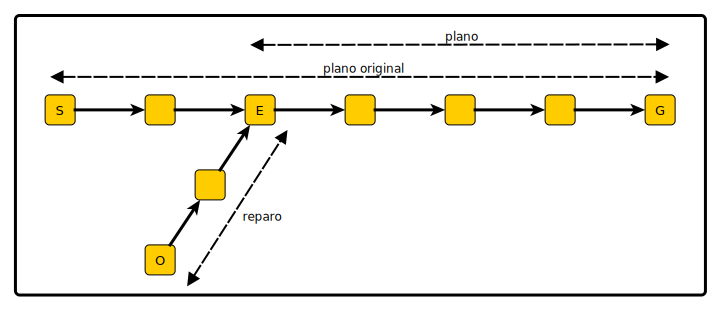
\includegraphics[scale=0.75,width=1.0\textwidth]{./img/exemplo_reparo_plano.ps} 
		\caption[Exemplo de reparo de plano]{Antes da execu��o o planejador apresenta um plano, aqui chamado de $plano\ original$, para ir de $S$ at� $G$. O agente executa o plano at� o ponto marcado com $E$. Antes de executar o $plano$ restante, ele verifica as pr�-condi��es e descobre que est�, de fato, no estado $O$. Em seguida, ele chama seu algoritmo de planejamento para apresentar um reparo, um plano para ir de $O$ at� algum ponto no $plano\ original$.}
    \end{figure}
\end{center}

A proposta desta disserta��o � abordar o m�todo de reparo de plano\index{reparo!de plano} de forma mais robusta, considerando o processo de repara��o a partir de duas opera��es distintas: ({\it 1}) remover a��es do plano que, no momento, tornam mais dif�cil atingir o(s) objetivo(s) e ({\it 2}) adicionar a��es que aproximem o agente do objetivo, sendo que a �ltima opera��o � muito similar ao planejamento cl�ssico. \\

\subsection{Trabalhos correlatos}

A utiliza��o de m�todos para reparo de plano, ao inv�s de se fazer o replanejamento, n�o � recente. Segue uma breve revis�o das principais propostas de reparo de plano encontradas na literatura:

\begin{itemize}

\item O \ac{GPG} \cite{Gerevini2000} � baseado em grafos de planos. Ele utiliza uma abordagem apoiada no planejador \cite{Blum1997} Graphplan. Quando o plano se torna in\-v�\-li\-do, o \ac{GPG} verifica onde ocorrem as inconsist�ncias do plano. O plano � ent�o dividido em tr�s partes: o topo do plano, que consiste em a��es que podem ser executadas a partir do estado inicial; uma parte intermedi�ria, que � composta por um conjunto de a��es inconsistentes e as a��es entre elas; e uma final, que pode ser utilizada para atingir os objetivos assim  que as inconsist�ncias tenham sido resolvidas. Estas tr�s partes podem ser identificadas utilizando-se o grafo de planejamento que foi constru�do durante a fase de planejamento. A parte intermedi�ria � ent�o descartada e um plano � procurado para preencher a lacuna existente entre o topo e o final do plano. Se este plano n�o puder ser encontrado a lacuna � ampliada e o processo � repetido. Eventualmente pode ocorrer de todo o plano ser descartado.  Neste caso, descarta-se a possibilidade de reparo e um plano completamente novo � constru�do, se for poss�vel. \\

% Este sistema n�o utiliza explicitamente um hist�rico. 
%Mas ao executar refinamentos reversos somente no plano inicial e nunca um dos
%planos produzidos por um passo do refinamento, isto pode ser visto como uma
%mem�ria impl�cita.
 
\item O modelo de planos do REPLAN \cite{Boella2002} � similar aos planos utilizados nos formalismos de \ac{HTN} \cite{Erol1994}. Uma rede de tarefas\index{rede de tarefas} descreve uma poss�vel forma de realizar uma tarefa por meio de sua decomposi��o em subtarefas ou, eventualmente, em a��es primitivas\index{a��o!primitiva} (ou seja, a��es que o agente pode executar de forma autom�tica). Para cada tarefa existe pelo menos uma destas redes de tarefas. Um plano � criado pela escolha da rede de tarefas correta para cada tarefa (abstrata), at� que cada rede contenha apenas a��es primitivas. Por meio deste processo de planejamento, o REPLAN constr�i uma �rvore de deriva��o\index{�rvore de deriva��o} que inclui todas as tarefas escolhidas e demonstra como um plano foi derivado. \\

O reparo de plano dentro do REPLAN � chamado de parti��o\index{parti��o}. Para cada n� inv�lido da �rvore de deriva��o, a (menor) sub-�rvore que cont�m este n� � removida. %(refinamento reverso).
Inicialmente, cada n� considerado inv�lido � uma a��o primitiva, e a raiz da �rvore correspondente � a tarefa que continha tal a��o. Subseq�entemente, um novo reparo � gerado para esta tarefa. Se o reparo falhar, uma nova etapa � iniciada, na qual sub-�rvores para tarefas hierarquicamente mais elevadas s�o removidas e regeradas. No pior caso esse processo continua at� que toda a �rvore de deriva��o seja descartada.  \\

%Como o GPG, REPLAN n�o faz refinamento reverso nunca um plano produzido pela
%etapa de refinamento, exceto para o plano  inicial. Novamente, isto pode ser
%visto como uma utiliza��o impl�cita da mem�ria.

%%%%%%%%%%%%%%%%%%%%%%%%%%%%%%%%%%%%%%%%%%%%%%%%%%%
% \item O SPA \cite{SPA} utiliza um tipo de busca local, iniciando com o
% plano % original. Ele tamb�m demonstra a separa��o em duas fases do reparo de
% plano. % Utiliza uma fila de planos parciais (implementando uma busca no
% espa�o de % planos) que podem ser utilizados em refinamento ou refinamento
% reverso. 
% adi��o ou remo��o de trechos.
% %Rotulando os planos na fila garante que o mesmo n�o seja visitado duas
% vezes, sendo assim considerado uma forma de mem�ria.
%%%%%%%%%%%%%%%%%%%%%%%%%%%%%%%%%%%%%%%%%%%%%%%%%%%

\item O O-Plan \cite{Drabble1997} utiliza a estrat�gia de regras para reparo de plano.
% Entretanto, n�o h� elementos como uma explica��o da falha.
Durante a execu��o o sistema confirma os efeitos de cada a��o. Para cada efeito que falha em que uma a��o � necess�ria para que outra seja executada, a��es adicionais, na forma de um reparo, s�o inclu�das no plano. Estes reparos de plano s�o planos pr�-constru�dos que podem reparar determinadas condi��es de falhas. Por exemplo, os planos de reparo podem incluir um plano para a troca de um pneu furado ou para a substitui��o de um motor quebrado. Quando uma condi��o incorreta � encontrada, a execu��o do plano � interrompida e um reparo de plano � inserido e executado. Ap�s a finaliza��o do reparo, a execu��o do plano regular recome�a. O O-Plan apenas adiciona a��es para reparar falhas e n�o emprega qualquer tipo de remo��o de a��es.
Deste modo, ele tamb�m � incompleto, pois nem todas as falhas podem  ser recuperadas. Xuemei Wang e Steve A. Chien \cite{Wang1997} descrevem como a busca pode ser incorporada ao O-Plan para tentar recuper�-lo de falhas\index{falha} para as quais nenhuma estrat�gia de reparo pr�-constru�da esteja dispon�vel. Entretanto, n�o considera a remo��o de a��es de um plano para a recupera��o das falhas, mas apenas para a descoberta de quais a��es precisam ser executadas novamente. \\

\end{itemize}
 %
%%%%%%%%%%%%%%%%%%%%%%%%%%%%%%%%%%%%%%%%%%%%%%%%%%%%%%%%%%%%%%%%%%%%%%%
\setlength{\parindent}{0pt}
\setlength{\textheight}{22cm}
\setlength{\parskip}{0.2cm}

% Para aumentar o espa�amento entre as linhas
\linespread{1.2}
%%%%%%%%%%%%%%%%%%%%%%%%%%%%%%%%%%%%%%%%%%%%%%%%%%%%%%%%%%%%%%%%%%%%%%%

\chapter{Reparo de plano por refinamento reverso}
\label{cap:reparo_de_plano_por_refinamento_reverso}

Este cap�tulo apresenta a estrat�gia de reparo de plano por refinamento reverso\index{refinamento!reverso} e do m�todo heur�stico\index{heur�stica} desenvolvido neste trabalho. 

\section{Refinamento reverso}

Para o reparo de plano n�o se pode utilizar diretamente o modelo de planejamento por refinamento, pois esta estrat�gia s� permite adicionar a��es, enquanto no reparo � preciso, al�m de adicionar, retirar a��es. O reparo de plano constitui de duas atividades distintas: a remo��o de a��es que estejam impedindo o sucesso do plano e a amplia��o do plano, por meio da adi��o de a��es (\cite{Roman2004}). Por este motivo, � necess�rio incluir uma {\it estrat�gia de refinamento reverso} para o reparo de plano. \\

A remo��o de restri��es do plano parcial impede que o plano atinja seus objetivos. A adi��o de a��es pode ser tratada como um planejamento normal, em que o plano parcial\index{plano!parcial} � ampliado (refinado) para satisfazer os objetivos. O Exemplo 5.1.1 ilustra uma situa��o em que apenas o reparo n�o � suficiente para que o plano atinja seu objetivo, sendo necess�rio um processo de refinamento reverso a fim de que o plano seja reparado. \\

\begin{Ex}
Suponha que exista um plano para um indiv�duo ir a um encontro utilizando um carro. Entretanto, ao se aproximar do carro, ele nota que um dos pneus est� furado. Um simples reparo para este plano poderia ser adicionar a��es para a troca do pneu por um sobressalente e, ent�o, prosseguir com o resto do plano, o que corresponderia � adi��o de a��es ao plano falho. Por�m, supondo que este � um encontro muito importante para o qual o indiv�duo n�o quer se atrasar e, neste caso, trocar o pneu poderia levar muito tempo, seria melhor remover do plano a a��o de dirigir o carro e substitu�-la por a��es que utilizem um t�xi. Nesse caso, algumas a��es do plano seriam removidas e outras, adicionadas. \\
\end{Ex}

Portanto, para reparar um plano, um planejador n�o deve apenas empregar
uma estrat�gia de refinamento\index{refinamento} com o intuito de ampliar o plano por meio de a��es que
atingir�o os objetivos. O planejador tem, tamb�m, que empregar uma
estrat�gia de {\it refinamento reverso\index{refinamento!reverso}} para diminuir as restri��es do
plano parcial (removendo a��es do plano que estejam obstruindo uma
solu��o). \\

% Em \cite{Roman2005} foi proposta uma heur�stica para o refinamento reverso que usa... . Por�m, n�o est� claro com... e como implementar tal heur�stica. 
%A heur�stica implementada nessa disserta��o usa algumas id�ias propostas pro Krogt, a saber:
%\begin{itemize}
 %\item cria uma vers�o relaxada do problema;
%\item desconsidera os efeitos negados;
%\item desconsidera as pr�-condi��es negadas. 
%\end{itemize}
%A diferen�a entre a heur�stica proposta aqui e a de Krogt � que a �rvore de de a��es a serem renovadas � enumerada...

No artigo \cite{Roman2005} os autores prop�em uma amplia��o do modelo do planejamento por refinamento que permite que estrat�gias de refinamento reverso sejam empregadas. A proposta original de Roman Krogt e Mathijs M. Weerdt pode ser melhor compreendida atrav�s da Figura 5.1.

\begin{center}
  \begin{figure}[ht!]
    \centering
	\label{fig:arquitetura_sistema_reparo_plano}
    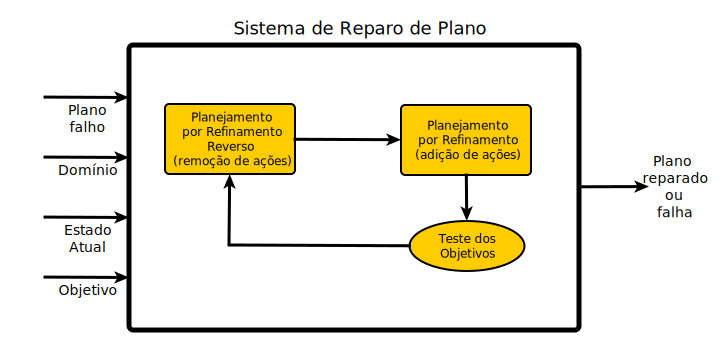
\includegraphics[angle=0,width=0.80\textwidth]{./img/sistema_reparo_plano.ps}
    \caption[Arquitetura de funcionamento do sistema de reparo de plano]{Arquitetura de funcionamento do sistema de reparo de plano.}
  \end{figure}
\end{center}

%% [TODO: 
%% o Historico so deve ser incluido no texto quando os algoritmos 
%% tamb�m tiverem suporte a historico. Isto �, que a funcao de heuristica
%% seja chamada mais de uma vez, e que ela tenha como parametro o historico
%% (H) para armazenar ate onde ja analisou;
%% ]

%A seguir,
%� introduzido um {\it hist�rico} $H$ para armazenar o caminho e os
%refinamentos reversos, a fim de ser capaz de prevenir {\it loops}
%inifinitos. A cada solicita��o de uma da heur�tica de refinamento reverso, �
%atualizado o hist�rico de modo a refletir que planos parciais j� foram
%considerados.

Uma vers�o adaptada desta proposta de amplia��o pode ser vista no Algoritmo \ref{algoritmo_reparo_plano}. Dado um plano $\pi$, parcialmente executado, o estado em que o plano apresentou falha, o dom�nio e a meta do problema, inicialmente, escolhe-se {\it refinar} o plano, isto �, adicionar refinamentos. Se n�o for encontrada uma solu��o, ent�o tenta-se {\it remover refinamentos} do plano. Para executar o modelo de refinamento reverso no plano, � necess�rio selecionar uma heur�stica de refinamento reverso e aplic�-la ao plano parcial. O refinamento ocorre no trecho do algoritmo referente ao planejamento normal. \\

O Algoritmo \ref{algoritmo_reparo_plano} funciona da seguinte forma: inicialmente ele atribui o estado em que a execu��o do plano original deveria estar caso n�o tivesse ocorrido a falha, a uma vari�vel ($e_g$). A seguir, o algoritmo chama um m�todo de planejamento que tenta encontrar um plano que leve a execu��o do estado atual $s$ ao estado desejado $e_g$, atribuindo o resultado a $\pi_r$. Na pr�xima fase, os comandos descritos nas linhas 4 e 5 verificam se o resultado $\pi_r$ � diferente de falha. Caso seja, o algoritmo devolve o reparo de plano encontrado pelo planejador concatenado ao plano original. Isto significa que somente a adi��o de novas a��es conseguiu reparar o plano falho. \\

Entretanto, caso o resultado de $\pi_r$ retorne uma falha, um m�todo heur�stico, que recebe como entrada o estado atual $s$ e o plano original $\pi$, � chamado. Este m�todo devolve como resposta uma estrutura de dados composta por uma lista de pares de {\tt estado} e {\tt quantidade}, que indica quais conjuntos de a��es do plano original devem ser considerados para a remo��o. A proposta � fazer com que a execu��o do plano retorne ao {\tt estado} do plano original ap�s a remo��o da {\tt quantidade} necess�ria de a��es. Ocorre, ent�o, um processo de repeti��o, onde cada par de {\tt estado} e {\tt quantidade} � testado a fim de que o plano saia do estado atual $s$ e consiga alcan�ar o estado $e_g$, atribuindo o resultado a $\pi_r$. \\

Os pr�ximos comandos verificam se o resultado $\pi_r$ � diferente de falha. Em caso afirmativo, remove-se do plano original a {\tt quantidade} de a��es. Em seguida o algoritmo devolve o reparo de plano encontrado pelo planejador concatenado ao plano original. Portanto, neste caso, para reparar o plano foi necess�ria a remo��o de um conjunto de a��es do plano original e a adi��o de um conjunto de novas a��es. Se nenhum dos pares for capaz de devolver uma resposta diferente de falha, ent�o um replanejamento\index{replanejamento} � feito. O m�todo de planejamento tenta encontrar um plano que saia do estado atual $s$ e consiga alcan�ar o objetivo $S_g$, atribuindo o resultado a $\pi_r$. Mais uma vez o algoritmo verifica se o resultado $\pi_r$ � diferente de falha. Caso seja, o algoritmo devolve o plano encontrado pelo planejador. \\

Uma vers�o do Algoritmo \ref{algoritmo_reparo_plano} sem heur�stica pode ser visualizada no Algoritmo \ref{algoritmo_reparo_plano_sem_heuristica}.

\begin{algorithm}
	\label{algoritmo_reparo_plano_sem_heuristica}
	\caption[Algoritmo de reparo de plano sem heur�stica]{Algoritmo de Reparo de Plano sem Heur�stica.}
	\Entrada{Trecho do plano original ainda n�o executado $\pi$, Estado atual $s$, Dom�nio $\mathcal{D}$, Objetivo $S_g$}
	\Saida{Plano reparado $\pi$ ou {\it falha}}
	\Inicio{
	$e_g \leftarrow $ recuperaEstado($\pi$)\;
	$\pi_r \leftarrow $ planejador($s$, $e_g$, $\mathcal{D}$)\;
	\Se{$\pi_r \ne $ {\it falha}}
		{{\bf devolve} $\pi_r + \pi$\;}
	\Senao{
		\Para{todos os conjuntos de a��es seq�enciais $c_a$ de $\pi$}{
			\Se{$\pi \ne c_a$}{
				$e_g \leftarrow $ recuperaEstado($\pi - c_a$)\;
				$\pi_r \leftarrow $ planejador($s$, $e_g$, $\mathcal{D}$)\;
				\Se{$\pi_r \ne $ {\it falha}}{
					$\pi \leftarrow \pi - c_a$\;
					{\bf devolve} $\pi_r + \pi$\;
				}
			}
		}
	}
	$\pi_r \leftarrow $ planejador($s$, $S_g$, $\mathcal{D}$)\;
	\Se{$\pi_r \ne $ {\it falha}}
		{{\bf devolve} $\pi_r$\;}
	{\bf devolve} $falha$\;
	}
\end{algorithm}

\begin{algorithm}
	\label{algoritmo_reparo_plano}
	\caption[Algoritmo de reparo de plano]{Algoritmo de Reparo de Plano.}
	\Entrada{Trecho do plano original ainda n�o executado $\pi$, Estado atual $s$, Dom�nio $\mathcal{D}$, Objetivo $S_g$}
	\Saida{Plano reparado $\pi$ ou {\it falha}}
	\Inicio{
	$e_g \leftarrow $ recuperaEstado($\pi$)\;
	$\pi_r \leftarrow $ planejador($s$, $e_g$, $\mathcal{D}$)\;
        \Se{$\pi_r \ne $ {\it falha}}
            {{\bf devolve} $\pi_r + \pi$\;}
        \Senao{
            lista[] $\leftarrow$ heur�stica($s$, $\pi$)\;
            \Repita{$lista[]$ estiver vazia}{
                $e_g \leftarrow $ lista.primeiroElemento().estado\;
		$\pi_r \leftarrow $ planejador($s$, $e_g$, $\mathcal{D}$)\;
                \Se{$\pi_r \ne $ {\it falha}}{
                    $\pi \leftarrow \pi$.remove($lista.primeiroElemento().quantidade$)\;
                    {\bf devolve} $\pi_r + \pi$\;
                }
                removePrimeiroElemento($lista[]$)\;
            }
	}
	$\pi_r \leftarrow $ planejador($s$, $S_g$, $\mathcal{D}$)\;
        \Se{$\pi_r \ne $ {\it falha}}
            {{\bf devolve} $\pi_r$\;}
	{\bf devolve} $falha$\;
    }
\end{algorithm}

\section{Heur�stica\index{heur�stica}} 
A forma mais comum de se adicionar conhecimento a respeito de um problema ao algoritmo de busca � por meio de fun��es heur�sticas. Uma fun��o heur�stica pode ser denotada por $h(n)$:

\begin{quote}
$h(n)\ =\ ${\small custo\ estimado\ do\ caminho\ mais\ econ�mico\ do\ n�\ $n$\ at�\ um\ n�\ objetivo.}
\end{quote}

Se $n$ � um n� objetivo, ent�o $h(n) = 0$. \\

Uma heur�stica � {\it admiss�vel\index{heur�stica!admiss�vel}} quando $h(n)$ 
n�o superestima o custo para alcan�ar o objetivo \cite{Russell2002}. Al�m disso, ela �
otimista por natureza, pois pressup�e que o custo da solu��o do problema �
 menor ou igual ao seu custo real. Isto ocorre porque a heur�stica ajuda a descartar os n�s de maior custo,
assegurando que o caminho �timo seja sempre o primeiro a ser escolhido. \\

Um modo de pensar sobre o problema da cria��o de heur�sticas � ter
como base um {\it problema relaxado}, no qual um problema � encarado com menos restri��es. O custo de
uma solu��o �tima para um problema relaxado � uma heur�stica\cite{Roman2005}
admiss�vel para o problema original \cite{Russell2002}. \\


A id�ia b�sica da constru��o de uma heur�stica para o planejamento reverso � observar os efeitos das a��es e os objetivos que
devem ser alcan�ados, e avaliar quantas a��es ser�o necess�rias para
alcan�ar todos os objetivos. \\

Uma sugest�o inicial � relaxar o problema removendo todas as
pr�-condi��es das a��es. Ent�o, toda a��o ser� aplic�vel e qualquer
literal poder� ser alcan�ado em um passo. \\

Uma heur�stica mais interessante seria, al�m de eliminar todas as pr�-condi��es: (1) eliminar os efeitos negativos das a��es e (2) considerar as intera��es positivas entre a��es. Isto �, se uma a��o tem o efeito $X\wedge \lnot Y$ no problema
original, ter� somente o efeito $X$ no problema relaxado, ou seja, nenhuma a��o pode excluir os literais alcan�ados por outro e, portanto, n�o � preciso se preocupar com intera��es negativas entre subplanos. Para que a uni�o dos efeitos
positivos dessas a��es satisfa�a o objetivo, calcula-se o
n�mero m�nimo de a��es necess�rias. Por exemplo, considere o objetivo ($X$, $Y$, $Z$) para o dom�nio descrito pelas as seguintes a��es:

\begin{quote}

a��o($\alpha$, EFEITO: $X\wedge Q$) \\
a��o($\beta$, EFEITO: $Y\wedge Z\wedge R$) \\
a��o($\delta$, EFEITO: $Y\wedge Q\wedge R$) 
\end{quote}

O conjunto de objetivos $\lbrace X, Y, Z \rbrace$ pode ser alcan�ado pelas a��es
$\lbrace \alpha, \beta \rbrace$ sendo a heur�stica igual a $2$, considerando custos unit�rios. � poss�vel notar que a a��o $\delta$ n�o � considerada, pois ela adiciona Y, que j� � inclu�do pela a��o $\beta$ (intera��o positiva).\\

A estrat�gia utilizada neste projeto foi gerar problemas
relaxados eliminando-se tanto as pr�-condi��es negativas quanto os efeitos negativos e ainda, considerando uma ordem total entre as a��es do plano para o c�lculo da heur�stica. \\

%Este tipo de heur�stica � classificada como {\it lista de elimina��o vazia} \cite{???}.

A abordagem para o uso destas heur�sticas de planejamento para reparo de planos � ilustrada na Figura 5.2.
%TODO: ~\ref{heuristica_refinamento}.
De um lado, temos o plano corrente $P$ que n�o ser� refinado. � computado, ent�o, o n�mero de planos que resulta da remo��o de a��es de $P$. Para cada um destes planos resultantes, utiliza-se uma heur�stica para estimar a quantidade de trabalho necess�ria para transformar este plano em um plano v�lido, isto �, calcula-se um valor heur�stico para cada um destes planos. O plano que obtiver o melhor (mais baixo) valor heur�stico � selecionado e o planejamento (refinamento) � utilizado para completar este plano. Se o planejador n�o puder produzir uma solu��o (o que pode acontecer porque a heur�stica n�o � perfeita), um outro refinamento reverso � escolhido. � importante notar que somente se aplica o passo do refinamento reverso ao plano inicial $P$. \\

Um outro ponto de vista importante sobre este procedimento que deve ser levado em considera��o � o espa�o de busca atravessado. Inicialmente, o m�todo de reparo de plano fornece o plano corrente $P$ para ser adaptado. Este plano pode estar localizado em uma parte do espa�o de busca em que � muito dif�cil encontrar uma solu��o por refinamento (isto �, adicionando apenas a��es), se tal solu��o existir. A heur�stica\index{heur�stica} de refinamento reverso avalia as condi��es do espa�o de busca ao redor destes planos parciais, isto �, calcula um valor heur�stico que expressa a facilidade com que o plano pode ser ampliado. Ap�s ser identificada a melhor op��o, � iniciado o processo de refinamento\index{refinamento}.

\begin{center}
    \begin{figure}[!ht]
		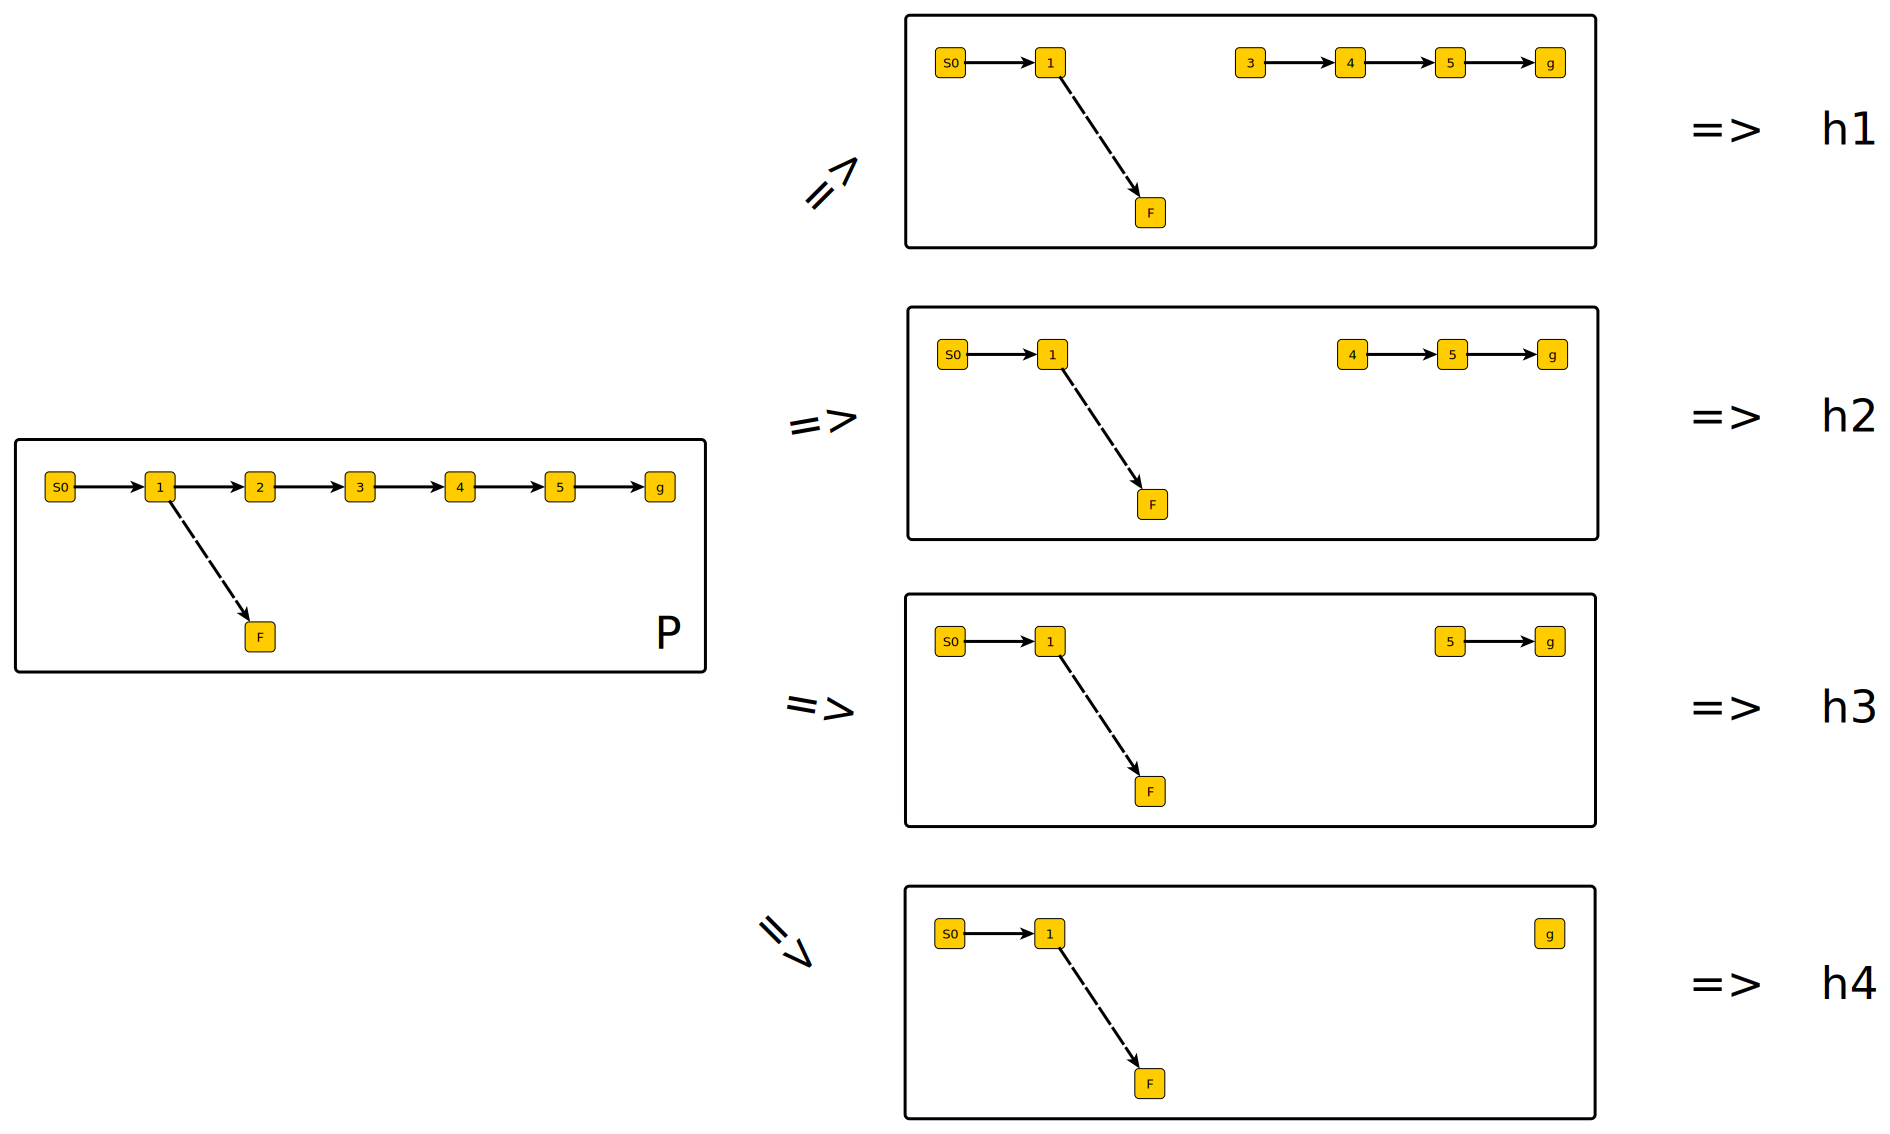
\includegraphics[angle=270, width=1.0\textwidth]{./img/heuristica.ps}
		\label{heuristica_refinamento} 
		\caption[Heur�stica para refinamento reverso]{Heur�stica de refinamento reverso. Do plano original � esquerda foram derivados $n$ subplanos e calculados seus respectivos valores heur�sticos ($h_1, \ldots, h_n$). A regi�o cinza representa a parte do plano que j� foi executada.}
		\end{figure}
\end{center}

A heur�stica\index{heur�stica} s� � utilizada nos casos em que o refinamento de plano falha ao tentar encontrar um reparo\index{reparo}. Seu objetivo � avaliar qual � o melhor conjunto de a��es a serem removidas, de modo que, a partir do novo estado inicial, possa ser encontrado um reparo, por meio de refinamento, que satisfa�a o novo estado-objetivo. \\

A heur�tica desenvolvida neste trabalho � baseada na remo��o de conjuntos de a��es seq�enciais e crescentes. Os conjuntos de a��es removidas a serem avaliados come�am com a primeira a��o n�o executada. A partir da�, cada novo conjunto � incrementado at� que todas as a��es tenham sido adicionadas. Inicia-se com uma a��o, depois duas e assim sucessivamente at� que todas as a��es sejam incorporadas. Para cada conjunto de a��es removidas um novo estado � gerado. Este estado cont�m
todas as pr�-condi��es necess�rias para executar todas as demais a��es (n�o removidas) at� o final do plano, como pode
ser observado na Figura 5.3.
%TODO: ~\ref{heuristica_refinamento_detalhado}.

\begin{center}
    \begin{figure}[!ht]  %\center
		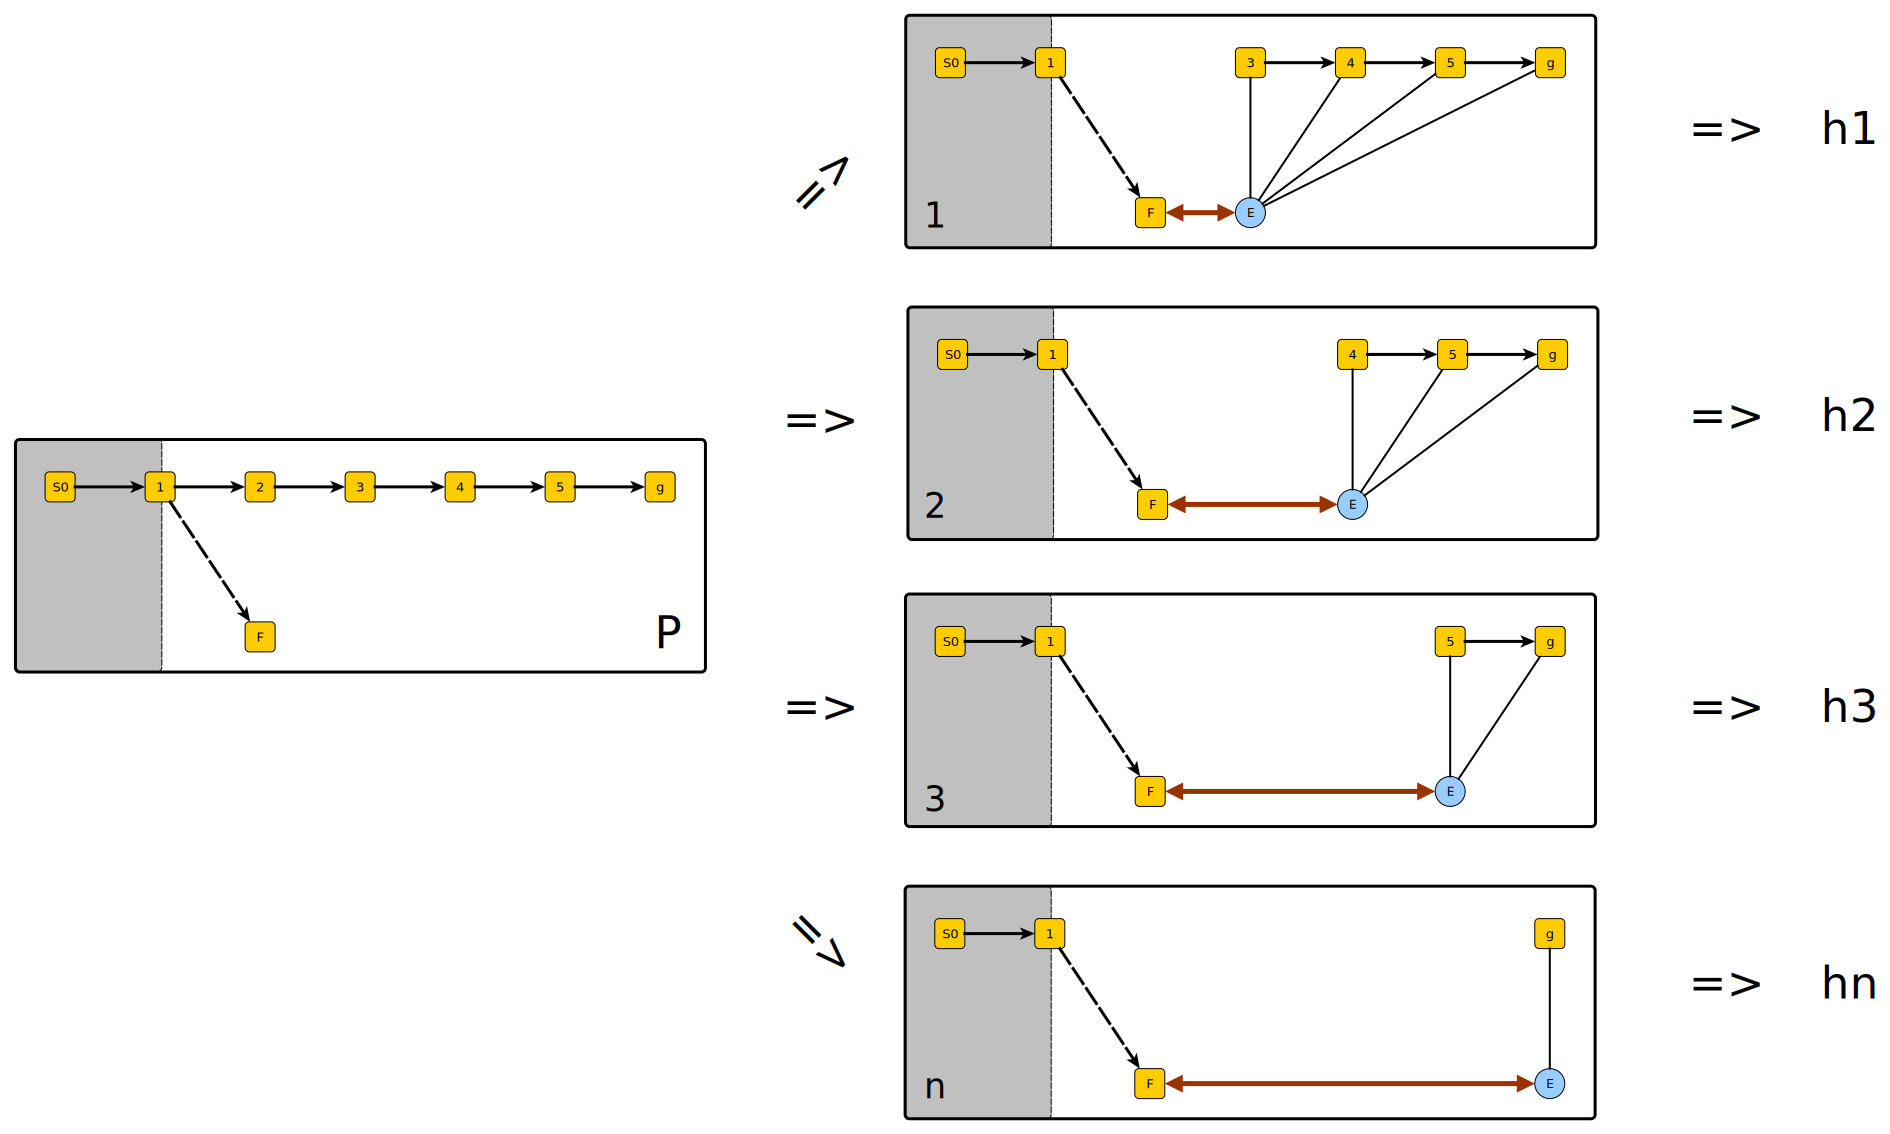
\includegraphics[angle=270, width=1.0\textwidth]{./img/heuristica2.ps}
		\label{heuristica_refinamento_detalhado} 
		\caption[Caracter�sticas da heur�stica para refinamento reverso]{Para cada conjunto de a��es removidas, um estado novo � gerado. Este estado cont�m todas as pr�-condi��es necess�rias para todas as a��es n�o removidas. A heur�stica calcula a dist�ncia entre o estado atual $F$ e o estado novo $E$. A regi�o cinza representa a parte do plano que j� foi executada.}
		\end{figure}
\end{center}

O Algoritmo \ref{heuristica} tem como objetivo devolver uma lista de pares de {\tt estado} e {\tt valor} e funciona da seguinte forma: para todos os conjuntos de a��es poss�veis de serem removidas, um estado com as condi��es necess�rias para executar o restante das a��es (n�o removidas) do plano original � gerado ($E_g$). O processo � iniciado, marcando-se como visitado o estado atual ($s$), e este � inserido na fila $s$ com o valor igual a $0$. Este valor serve para indicar a dist�ncia entre o estado atual e o estado inserido na fila. A partir da linha 6 at� a linha 19, para cada elemento $f$ da $fila$, verifica se o mesmo est� contido em $E_g$. Se estiver, insere na lista de $resultados$, e o algoritmo devolve $resultados$ se tiver $E_g$ contido. Seq�encialmente, entre as linhas 12 e 18, para todas as a��es $a$ aplic�veis ao estado $f.estado$, atribui a $s_{novo}$ o estado resultante ap�s a execu��o da a��o (linha 15). Sendo que esta execu��o n�o considera os efeitos negativos da a��o. Verifica se o estado $s_{novo}$ n�o est� marcado como visitado. Caso n�o esteja, marca como visitado e insere na $fila$ com o valor de $f.valor$ incrementado em um. Deste modo a estrutura da fila ter� um conjunto de estados e valores que indicam a dist�ncia em rela��o ao estado atual $s$. (linha 16 a 18). Sendo que o conjunto de elementos devolvidos pelo algoritmo estar� ordenado de acordo com o $valor$ heur�stico atribu�do. \\



\begin{algorithm}
	\label{heuristica}
	\caption[Heur�stica para refinamento reverso]{Heur�stica para Refinamento Reverso}
	\Entrada{Estado Atual $s$, Plano Original $\pi$}
	\Saida{Lista de pares de {\it Estado e valor}}
	\Inicio{
        $E_g \leftarrow$ geraListaEstados($\pi$)\;
        \ \\ %lista$<$valor, Estado$>$ fila[], resultado[]\;

        visitado($s$)\;
        fila.insere($0$, $s$)\;

        \Repita{fila estiver vazia}{
            $f \leftarrow$ fila.retiraIn�cio()\;
            \Se{$f$.estado $\subset E_g$.estado}{
                resultado.insere($f$)\;
                \Se{$E_g \subseteq$ resultado}{
                    {\bf devolve} resultado\;
                }
            }
            \Para{toda a��o $a$ aplic�vel ao estado $f$.estado}{
                {\small
                // Executa a a��o $a$ no estado $f.estado$ \\
                // sem considerar efeitos negativo 
                } \\
                $s_{novo} \leftarrow$ executa($f$.estado, $a$)\;
                \Se{n�o visitado($s_{novo}$)}{
                    visitado($s_{novo}$)\;
                    fila.insere($f$.valor $+ 1$, $s_{novo}$)\;
                }
            }
        }
	{\bf devolve} resultado\;
    }
\end{algorithm}

%A estrat�gia da heur�stica\index{heur�stica} utilizada para refinamento reverso\index{refinamento!reverso} funciona da seguinte forma: ap�s ter sido gerado um conjunto de estados $E_g$ baseados nos grupos de a��es removidas, marca-se o estado atual como visitado e o insere com valor es\-pe\-c�\-fi\-co (iniciado com $0$) na fila de estados a serem analisados. Este valor indica a dist�ncia entre o estado atual e o estado inicial e o grau de dificuldade entre os dois estados. \\
%
%Em seguida, o algoritmo entra em um bloco de repeti��o, onde fica at� que ocorra uma interrup��o, uma vez que j� se calculou a dist�ncia entre todos os estados-objetivo, ou porque n�o existe mais nenhum elemento na fila de estados a ser analisado, de modo que a cada itera��o do bloco de repeti��o � retirado o primeiro elemento da fila para an�lise. Inicialmente, deve-se verificar se o elemento faz parte do conjunto de $E_g$. Em caso afirmativo, ele � adicionado a um conjunto de resultados. O conjunto de resultados, assim como a fila de estados a serem analisados, cont�m o valor que indica a dist�ncia entre o estado atual e o estado inicial. \\
%
%A an�lise das poss�veis alternativas � feita da seguinte maneira: para todas as a��es aplic�veis ao elemento atual, executa-se uma a��o sem considerar os efeitos negados. Se o novo estado resultante da execu��o ainda n�o tiver sido visitado, deve-se marc�-lo como visitado e adicion�-lo � fila de estados, com o valor es\-pe\-c�\-fi\-co do elemento corrente incrementado em um. \\


%%%%%%%%%%%%%%%%%%%%%%%%%%%%%%%%%

%O sistema de reparo de plano por refinamento reverso � uma t�cnica ainda pouco explorada na �rea de planejamento. Um dos estudos realizados nesta �rea envolve o sistema \ac{POPR}\index{POPR} desenvolvido por Roman Krogt e Mathijs M. Weerdt.  \\

%No artigo \cite{Roman2005} os autores prop�em uma maneira de utilizar o planejador VHPOP, com algumas modifica��es, para escolher quais a��es devem ser removidas do plano a fim de que ele atinja seus objetivos. Entretanto, este sistema n�o se encontra dispon�vel para dom�nio p�blico. \\





%%%%%%%%%%%%%%%%%%%%%%%%%%%%%%%%%%%%%%%%%%%%%%%%%%%%%%%%%%%%%%%%%%%%%%%
\setlength{\parindent}{0pt}
\setlength{\textheight}{22cm}
\setlength{\parskip}{0.2cm}

% Para aumentar o espa�amento entre as linha
\linespread{1.2}
%%%%%%%%%%%%%%%%%%%%%%%%%%%%%%%%%%%%%%%%%%%%%%%%%%%%%%%%%%%%%%%%%%%%%%%

\chapter{Implementa��o e an�lise experimental}
\label{cap:implementacao_e_analise_experimental}

Como foi dito no Cap�tulo \ref{cap:reparo_de_plano_por_refinamento_reverso}, n�o existe uma implementa��o dispon�vel de um sistema de reparo de plano por refinamento reverso. Assim, um dos objetivos deste trabalho � implementar um sistema de reparo desse tipo para disponibiliz�-lo, bem como para verificar empiricamente as situa��es em que o reparo de plano pode ser mais vantajoso do que o replanejamento e como o uso da heur�stica pode melhorar sua efici�ncia. \\

%O sistema de reparo de plano por refinamento reverso � uma t�cnica ainda pouco explorada na �rea de planejamento. Um dos estudos realizados nesta �rea envolve o sistema \ac{POPR}\index{POPR} desenvolvido por Roman Krogt e Mathijs M. Weerdt. 

%No artigo \cite{Roman2005} os autores prop�em uma maneira de utilizar o planejador VHPOP, com algumas modifica��es, para escolher quais a��es devem ser removidas do plano a fim de que ele atinja seus objetivos. Entretanto, este sistema n�o se encontra dispon�vel para dom�nio p�blico. \\

%Tomando como base o sistema descrito no artigo \cite{Roman2005}, foi implementado, o processo de refinamento reverso. No presente cap�tulo, mais especificamente, s�o colocadas em pr�tica as t�cnicas de reparo de plano apresentadas nas se��es anteriores, a fim de possibilitar uma compara��o emp�rica com outras abordagens. Foi desenvolvido um simulador, que interage com o sistema de reparo e reproduz as a��es de um agente em um ambiente din�mico, o qual p�de ser reproduzido devido a um gerador de falhas, criado exclusivamente para este fim. A intera��o entre o sistema de reparo, o simulador e o gerador de falhas produziu um conjunto de resultados experimentais aqui apresentados.\\

\section{Sistema de reparo de plano}

O sistema de reparo de plano por refinamento reverso implementado neste trabalho utiliza como base o \ac{VHPOP}\index{VHPOP}, um planejador de c�digo fonte\index{c�digo fonte} aberto que implementa de forma expl�cita o planejamento por refinamento. O \ac{VHPOP} foi desenvolvido por H�kan Younes e R.G. Simmons na Universidade Carneguie Mellon em 2003 \cite{Younes2003} em C++\index{C++}. Originalmente, o planejador \ac{VHPOP} recebe como entrada tr�s conjuntos de dados: o dom�nio\index{dom�nio}, o estado inicial e o objetivo. Todos os dados de entrada est�o no formato {PDDL}. Ao executar o sistema\index{sistema}, o planejador produz, se existir, um plano resposta para o problema (Figura 6.1). \\

\begin{figure}[!ht] % Figura 6.1
    \centering
    \label{fig:vhpop}
    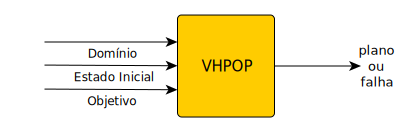
\includegraphics[angle=0,width=0.80\textwidth]{./img/vhpop.ps}
    \caption[Arquitetura de funcionamento do VHPOP]{Arquitetura de funcionamento do VHPOP.}
\end{figure}

O sistema de reparo implementado (Figura 6.2) recebe como entrada:

\begin{itemize}
 \item um plano falho, com indica��o das a��es j� executadas;
 \item uma descri��o do dom�nio (conjunto de a��es do agente);
 \item o estado atual da simula��o;
 \item uma descri��o dos estados objetivos.
\end{itemize}

Tal sistema devolve como resposta uma falha, se um reparo n�o for encontrado, caso contr�rio, uma resposta v�lida ser� uma seq��ncia de a��es que atinja o objetivo do problema.

%Entretanto, uma resposta v�lida da execu��o do sistema de reparo de plano por
%Pode acontecer do VHPOP-RE n�o
%encontrar um reparo\index{reparo}, pois uma falha\index{falha} pode levar a simula��o do sistema a um
%estado {\it sem sa�da}, isto �, um estado a partir do qual n�o exista um plano que
%alcance o objetivo do problema inicial. \\ 

%%% ---> No trabalho do Perseke � falado sobre o assunto de becos sem sa�da! <--- %%%%

%refinamento reverso devolver� uma seq��ncia de a��es. Ao ser executada a
%seq��ncia de a��es devolvida pelo sistema, a simula��o sair� do estado
%corrente e alcan�ar� um estado que faz parte da execu��o do plano original. \\

\begin{figure}[!ht] % Figura 6.2
    \centering
    \label{fig:vhpop_re}
    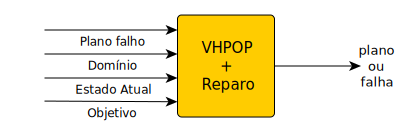
\includegraphics[angle=0,width=0.80\textwidth]{./img/vhpop-re.ps}
    \caption[Sistema VHPOP-RE]{Sistema VHPOP-RE.}
\end{figure}


O sistema de reparo pode ser executado com ou sem o uso de heur�stica. O sistema sem o uso de heur�stica (Algoritmo \ref{algoritmo_reparo_plano_sem_heuristica} do Cap�tulo \ref{cap:reparo_de_plano_por_refinamento_reverso}) chamado de VHPOP-RE,  testa todas as alternativas poss�veis para encontrar a solu��o �tima de reparo. A vers�o com heur�stica (Algoritmo \ref{heuristica} do Cap�tulo \ref{cap:reparo_de_plano_por_refinamento_reverso}), chamada de VHPOP-RE-H, tenta encontrar um reparo fazendo o menor n�mero de tentativas. Com isso, espera-se que esse seja um m�todo mais eficiente de reparo de planos.\\

Os sistemas VHPOP-RE e VHPOP-RE-H foram implementados de forma a encapsular completamente o planejador \ac{VHPOP} (Figura 6.3): a id�ia � que ap�s remover a��es do plano por refinamento reverso, esses sistemas usem o pr�prio VHPOP para completar o plano. \\

\begin{center}
  \begin{figure}[ht!] % Figura 6.3
    \centering
	\label{fig:arquitetura_vhpop-re}
    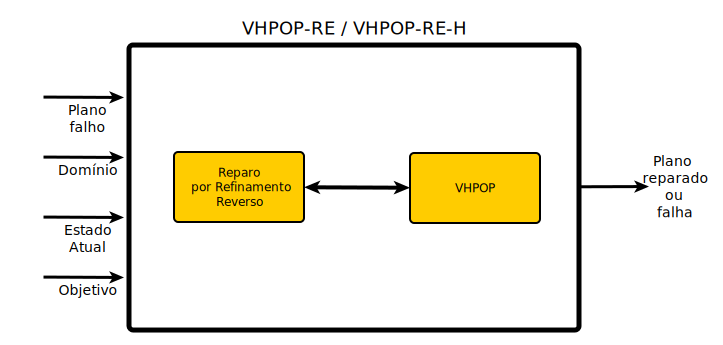
\includegraphics[angle=0,width=0.80\textwidth]{./img/sistema_reparo_plano_vhpop-re.ps}
    \caption[Arquitetura de funcionamento do VHPOP-RE]{Arquitetura de funcionamento do VHPOP-RE.}
  \end{figure}
\end{center}

\section{Simulador da din�mica de ambientes de teste}

Al�m da implementa��o do VHPOP-RE, foi desenvolvido um sistema de simula��o da din�mica de ambientes de planejamento para testar o sistema de reparo, chamado de SIMULA-PLANO\index{SIMULA-PLANO}. Este sistema tem como objetivo simular a execu��o de planos em diferentes dom�nios, com a possibilidade de simular falhas durante a execu��o de um plano.

O simulador recebe como entrada:
\begin{itemize}
 \item uma descri��o do dom�nio (conjunto de a��es do agente);
 \item o estado inicial do ambiente;
 \item um plano para atingir o objetivo do agente;
 \item um conjunto de falhas.
% e o momento espec�fico em que se deseja que elas sejam executadas; 
\end{itemize}

%Al�m destes dados, � poss�vel tamb�m configurar o simulador para que este execute todos os procedimentos de modo autom�tico, ou de modo interativo, em que a cada etapa � necess�rio que o usu�rio intervenha na execu��o. \\

O conjunto de falhas pode ser informado ao simulador de duas maneiras diferentes: (1) pelo programa de gera��o de falhas autom�ticas Se��o \ref{cap:6:sec:o_sistema_de_geracao_de_falhas}, ou (2) pela interven��o de um usu�rio. \\

Durante a execu��o de um plano, o simulador verifica as pr�-condi��es de todas as a��es a serem executadas. Ao detectar que uma ou mais  pr�-condi��es n�o s�o satisfeitas, o simulador chama o sistema VHPOP-RE. \\

% \subsection{Interface Web}

Com o intuito de facilitar a visualiza��o, foi desenvolvida uma interface Web\index{interface web} que permite observar a execu��o das a��es do plano com a ocorr�ncia de falhas e as a��es de reparo, bem como permite que o usu�rio interaja com o simulador para a gera��o de falhas. A Figura 6.4
%TODO: ~\ref{fig:screenshot_simulador}
apresenta uma imagem da interface Web durante a execu��o de um plano no simulador.
� poss�vel visualizar a ocorr�ncia de uma falha que inviabiliza as pr�-condi��es da a��o {\tt A1}, uma vez que o estado passou do estado {\tt S1} ao {\tt SR0}. A partir deste ponto um reparo de plano � executado (a��es {\tt AR0}, {\tt AR1} e {\tt AR2}) at� retomar o plano original a partir da a��o {\tt A2}.

\begin{figure}[ht!] % Figura 6.4
    \centering
	\label{fig:screenshot_simulador}
    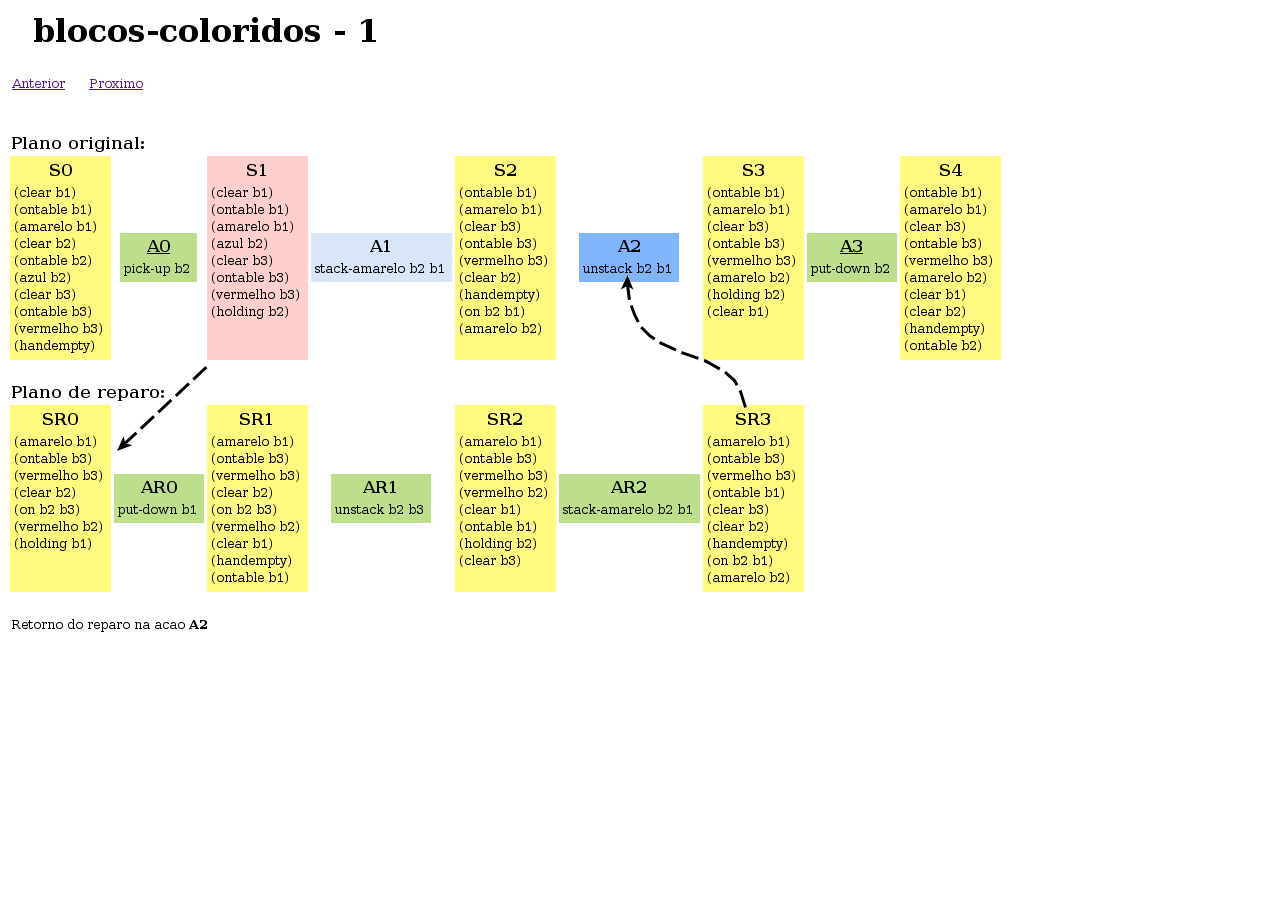
\includegraphics[angle=90,height=0.90\textheight]{./img/screen_shot_simulador.ps}
    \caption[Simula��o de execu��o do plano]{O plano original � mostrado acima  do reparo. A��es j� executadas do plano original aparecem com nomes sublinhados. A��es removidas do plano original s�o ilustradas por ret�ngulos de cor cinza claro. As setas sobrepostas � foto da tela indicam em que ponto do plano original ocorreu a falha, e qual � o ponto da retorno ap�s a execu��o do reparo.}
\end{figure}

%\begin{figure}[ht!]
%    \centering
%	\label{fig:screenshot_simulador}
%    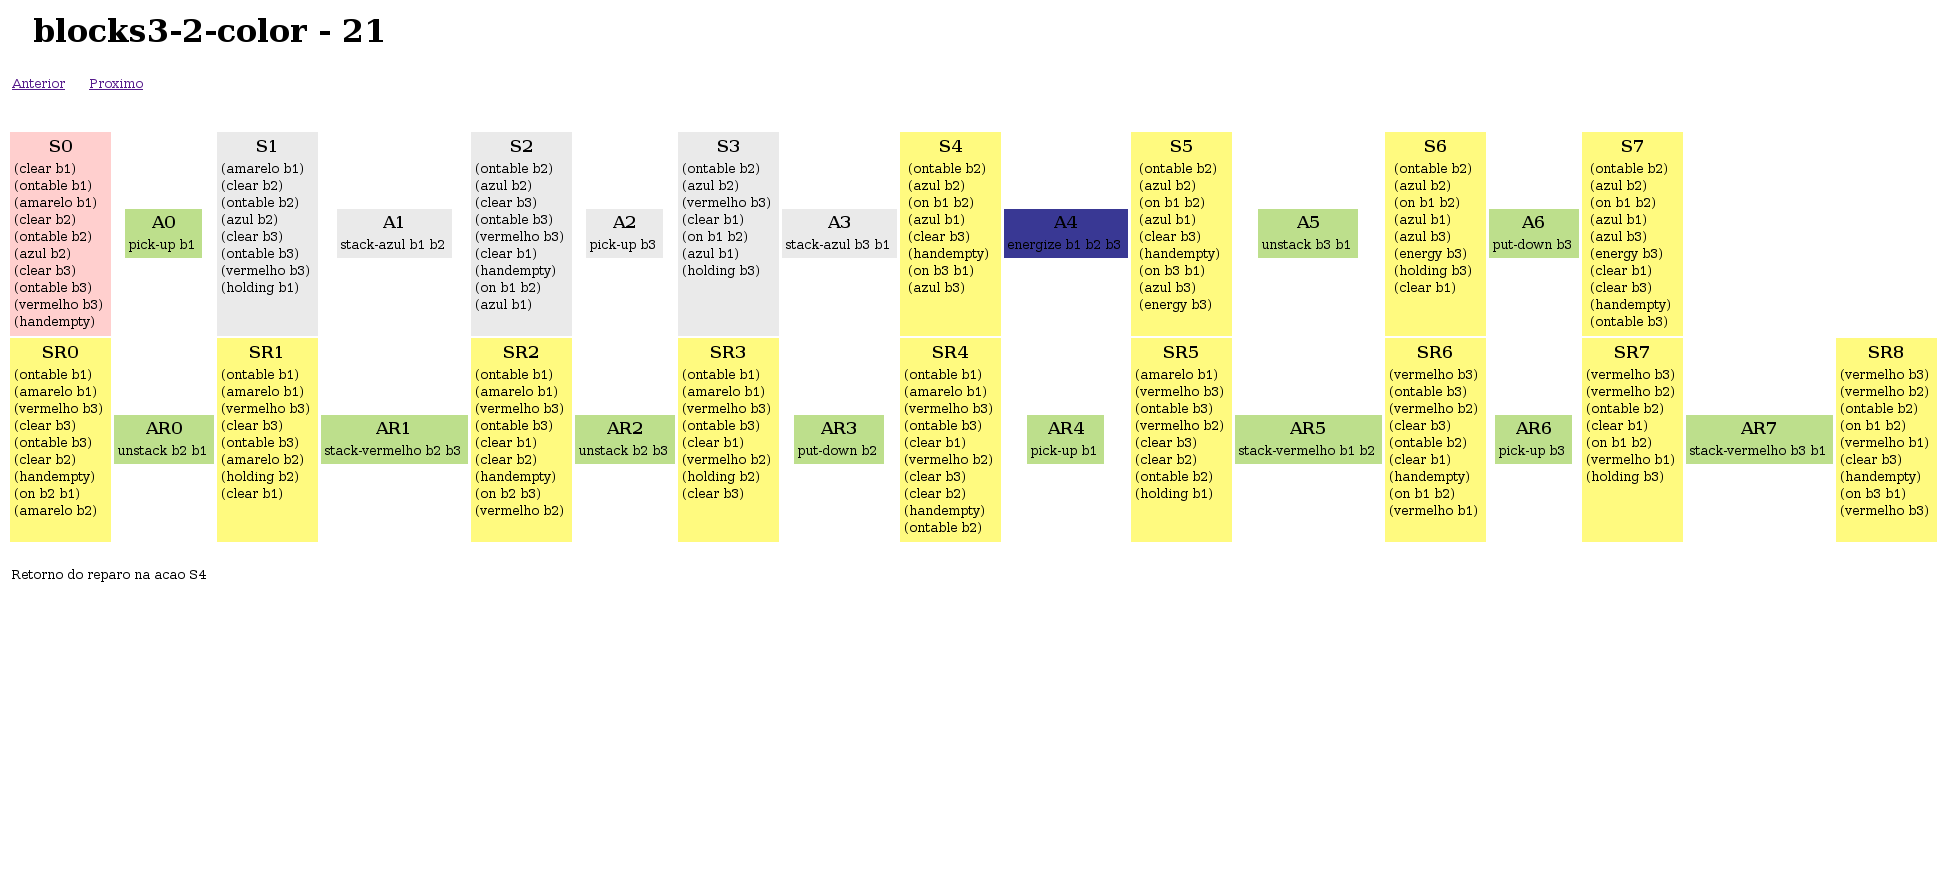
\includegraphics[angle=0,width=1.0\textwidth]{./img/screenshot_simulador_2.ps}
%    \caption{Imagem da tela durante a execu��o do simulador observado pela
%interface Web.}
%\end{figure}

\section{O programa de gera��o de falhas}
\label{cap:6:sec:o_sistema_de_geracao_de_falhas}

Para que os testes pudessem ser realizados foi criado um sistema de gera��o de falhas independente de dom�nio.
Criar uma altera��o espec�fica significa simplesmente invalidar uma pr�-condi��o e ainda manter um estado consistente. Por exemplo, no dom�nio do Mundo dos Blocos, ao tentar desempilhar um bloco, uma das pr�-condi��es � que o bloco esteja livre, uma altera��o espec�fica colocaria um outro bloco sobre o bloco que se quer desempilhar, para cria uma falha.
Um dos cuidados que se deve ter � de manter a consist�ncia dos estados: simplesmente fazer com que uma pr�-condi��o se torne falsa, pode gerar estados inconsistentes. Por exemplo, se o $Bloco_A$ estiver sobre o $Bloco_B$, n�o se pode adicionar a condi��o $Livre(Bloco_B)$, sem adicionar a condi��o $Sobre(Bloco_A, mesa)$ ou $Sobre(Bloco_A, Bloco_C)$, isto �, o $Bloco_A$ deve estar em outro lugar que n�o seja sobre o $Bloco_B$.\\

Sendo assim, a alternativa para manter estados conscientes � executar a��es ex�genas\footnote{A��es ex�genas podem ser as mesmas a��es do dom�nio, por�m, elas s�o supostamente executadas por outro agente que tem como objetivo invalidar os planos do agente principal e por isso podem tamb�m ser chamadas de a��es ex�genas.}\index{a��o!ex�gena} cujos efeitos inviabilizem ao menos uma das pr�-condi��es da a��o. O programa de gera��o de falhas realiza os seguintes passos:

\begin{enumerate}
 \item sorteia (ou seleciona) uma a��o $a_f$ para falhar;
\item seleciona uma ou mais pr�-condi��es de $a_f$ que ser�o negadas, $p \subseteq$ pr�-condi��es ($a_f$);
\item chama o VHPOP, o qual recebe como entrada o subconjunto $p$, o estado $s$ anterior � execu��o de $a_f$, o dom�nio; e devolve como sa�da um plano de a��es ex�genas; 
\item solicita ao simulador que execute o plano de a��es ex�genas imediatamente antes da execu��o de $a_f$.
\end{enumerate}


%A Figura 6.? ilustra a gera��o de falha utilizando as tr�s t�cnicas. \\

%\begin{center}
%\begin{figure}[ht!] % Figura 6.?
%    \centering
%    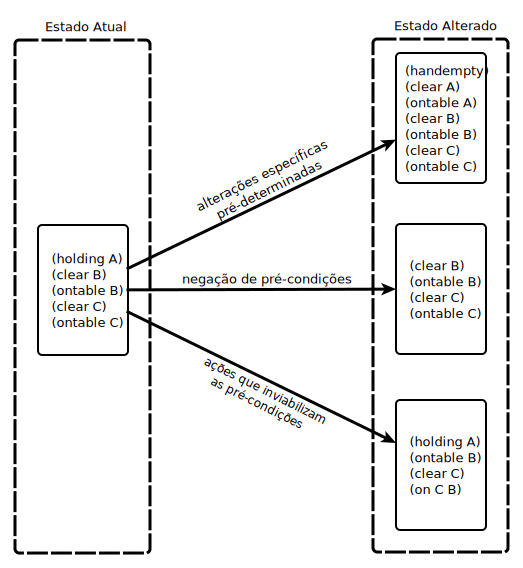
\includegraphics[angle=0,width=0.6\textwidth]{./img/geracao_falhas.ps}
%    \caption[Exemplo de gera��o de falha]{A partir do estado atual, deseja-se fazer com que a a��o {\it empilhar} ({\it stack}, descrita no Ap�ndice \ref{apendice_dominio_blocos}) falhe. Neste exemplo as tr�s t�cnicas s�o aplicadas, gerando diferentes estados. � poss�vel visualizar que o m�todo de nega��o das pr�-condi��es cria um estado inconsistente, pois o bra�o mec�nico n�o est� segurando nada, mas tamb�m n�o est� livre. Al�m disso, n�o h� qualquer informa��o sobre o {\tt bloco A}.}
%\end{figure} 
%\end{center}

% Entretanto, � poss�vel que n�o haja um conjunto de a��es que inviabilize as pr�-condi��es da a��o escolhida, ou que tal conjunto seja muito grande. Portanto, delimitou-se a busca a um n�mero m�ximo de a��es. Caso esta busca n�o encontre nenhum conjunto que satisfa�a o objetivo, uma outra a��o � escolhida de forma aleat�ria e o processo recome�a. \\

% As falhas geradas possuem informa��es que permitem ao simulador\index{simulador} aplic�-las em determinado instante durante a execu��o do plano. Desta forma torna-se vi�vel realizar uma an�lise emp�rica sobre a implementa��o do sistema de reparo de
%plano por refinamento reverso, pois � poss�vel aplicar a mesma falha nas diferentes situa��es propostas por esta disserta��o. \\

\section{A arquitetura do sistema}

Os sistemas VHPOP-RE\index{VHPOP-RE}, VHPOP-RE-H e o simulador foram implementados na linguagem de programa��o C++\index{C++}, gerando aproximadamente 5300 linhas de c�digo. A interface Web do simulador foi implementada utilizando a linguagem de programa��o Perl\index{Perl}. \\
% e gerou aproximadamente 900 linhas de c�digo, desconsiderando os templates em \ac{HTML}\index{HTML}. \\

A Figura 6.5
%TODO: ~\ref{arquitetura} 
ilustra a arquitetura e dados trocados entre cada segmento do sistema.
%O simulador recebe como entradas um conjunto de falhas, o plano pr�-determinado pelo planejador, bem como o dom�nio e o problema a ser solucionado. Ap�s a simula��o, ele devolve ao sistema de reparo o status da execu��o das a��es. De acordo com as respostas do simulador, o sistema de reparo tomar� decis�es a respeito de como proceder em cada caso. A interface Web permite a monitora��o visual dos estados e a��es que foram executadas no simulador.
Mais detalhes da implementa��o podem ser vistos no Ap�ndice \ref{apendice_arquitetura_sistema}, o qual mostra o Diagrama de Classe\index{Diagrama!de Classe} em {UML}. \\

\begin{center}
  \begin{figure}[ht!] % Figura 6.5
    \centering
	\label{arquitetura}
    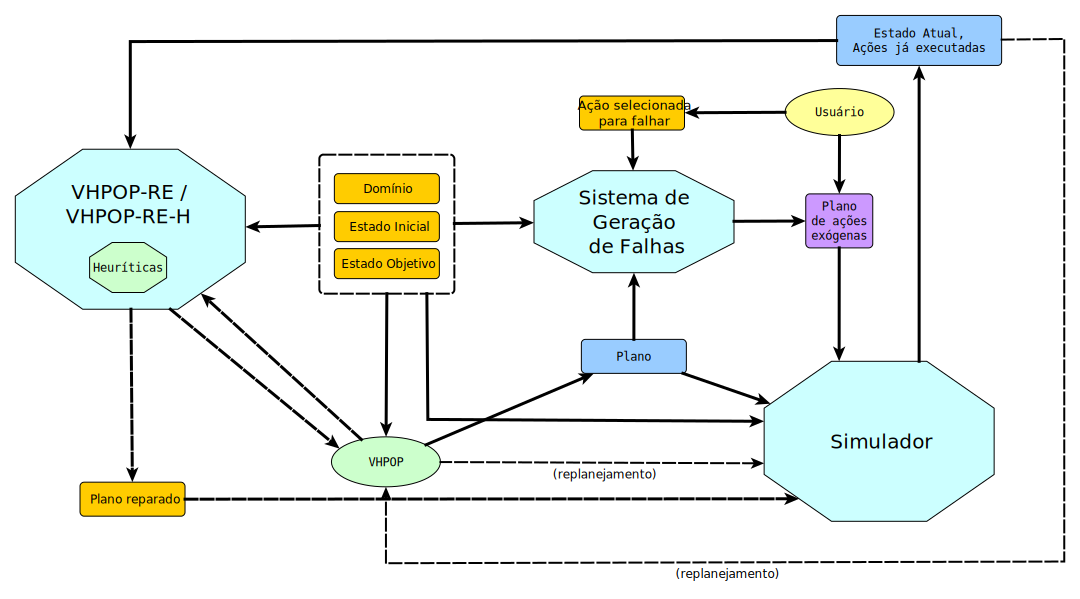
\includegraphics[angle=270,width=1.0\textwidth]{./img/arquitetura_implementada.ps}
    \caption[Arquitetura do sistema de reparo]{Arquitetura do sistema de reparo de plano por refinamento reverso. Os oct�gonos representam os sistemas implementados nesse trabalho.}
  \end{figure}
\end{center}



\section{Dom�nios de teste}

Os dom�nios\index{dom�nio} de teste utilizados nesta disserta��o s�o inst�ncias dos dom�nios: Mundo dos Blocos Coloridos\index{Mundo dos Blocos Coloridos} e Controle de Sat�lites\index{Controle de Sat�lites}. \\

\subsection{Mundo dos Blocos Coloridos}

O dom�nio do Mundo dos Blocos Coloridos � uma varia��o do dom�nio do Mundo dos Blocos \cite{Winston1992} que foi definido nessa disserata��o para testar problemas interessantes de reparo de planos. \\ 

A diferen�a entre esses dois dom�nios � que no Mundo dos Blocos Coloridos, al�m de cada bloco possuir uma identifica��o �nica, ele possui uma cor pr�-determinada. Ao empilhar um bloco sobre o outro, o bloco superior assume a cor do bloco inferior e, mesmo que os blocos sejam separados, a modifica��o de cor permanecer� at� que o bloco seja disposto em cima de um outro bloco de cor diferente e uma nova altera��o ocorra. Um exemplo deste dom�nio pode ser visto na Figura 6.6,
%TODO: ~\ref{fig:mundo_blocos_coloridos}, 
e sua descri��o encontra-se na Tabela \ref{tab:dominio_blocos_coloridos}. \\

\begin{figure}[ht!] % Figura 6.6
    \centering
	\label{fig:mundo_blocos_coloridos}
    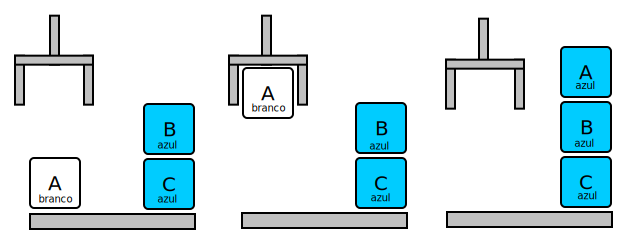
\includegraphics[angle=0,width=1.0\textwidth]{./img/mundo_blocos_coloridos.ps}
    \caption[Mundo dos Blocos Coloridos]{Este exemplo mostra o comportamento
da a��o empilhar no Mundo dos Blocos Coloridos. Ao empilhar o bloco branco A sobre o bloco azul B, o bloco A muda da cor branca para a cor azul.}
\end{figure}

\begin{Tab}{Descri��o das a��es no dom�nio do Mundo dos Blocos Coloridos}
\label{tab:dominio_blocos_coloridos}
\begin{center}
% use packages: array
\begin{tabular}{|c|l|l|}
\hline
\multicolumn{2}{|c|}{\textbf{A��o}} & \textbf{Descri��o} \\ \hline \hline

\multicolumn{3}{|l|}{\tt \scriptsize pick-up(?x)} \\ \hline
\multicolumn{2}{|r|}{\tt \scriptsize precondi��o:} & \tt \scriptsize (and (clear ?x) (ontable ?x) (handempty)) \\
\multicolumn{2}{|r|}{\tt \scriptsize efeito:}      & \tt \scriptsize (and (not (ontable ?x)) (not (clear ?x))  \\
\multicolumn{2}{|r|}{\tt \ }           & \tt \scriptsize (not (handempty)) (holding ?x)) \\
\hline \hline

\multicolumn{3}{|l|}{\tt \scriptsize put-down(?x)} \\ \hline
\multicolumn{2}{|r|}{\tt \scriptsize precondi��o:} & \tt \scriptsize (holding ?x) \\
\multicolumn{2}{|r|}{\tt \scriptsize efeito:}      & \tt \scriptsize (and (not (holding ?x)) (clear ?x) (handempty) \\
\multicolumn{2}{|r|}{\tt \ }           & \tt \scriptsize (ontable ?x)) \\
\hline \hline

\multicolumn{3}{|l|}{\tt \scriptsize stack-amarelo(?x ?y)} \\ \hline
\multicolumn{2}{|r|}{\tt \scriptsize precondi��o:} & \tt \scriptsize (and (holding ?x) (clear ?y) (amarelo ?y)) \\
\multicolumn{2}{|r|}{\tt \scriptsize efeito:}      & \tt \scriptsize (and (not (holding ?x)) (not (clear ?y)) \\
\multicolumn{2}{|r|}{\tt \ }           & \tt \scriptsize (clear ?x) (handempty) (on ?x ?y) \\
\multicolumn{2}{|r|}{\tt \ }           & \tt \scriptsize (amarelo ?x) (not (azul ?x)) \\
\multicolumn{2}{|r|}{\tt \ }           & \tt \scriptsize (not (vermelho ?x))) \\
\hline \hline

\multicolumn{3}{|l|}{\tt \scriptsize stack-azul(?x ?y)} \\ \hline
\multicolumn{2}{|r|}{\tt \scriptsize precondi��o:} & \tt \scriptsize (and (holding ?x) (clear ?y) (azul ?y)) \\
\multicolumn{2}{|r|}{\tt \scriptsize efeito:}      & \tt \scriptsize (and (not (holding ?x)) (not (clear ?y)) \\
\multicolumn{2}{|r|}{\tt \ }           & \tt \scriptsize (clear ?x) (handempty) (on ?x ?y) \\
\multicolumn{2}{|r|}{\tt \ }           & \tt \scriptsize (not (amarelo ?x)) (azul ?x) \\
\multicolumn{2}{|r|}{\tt \ }           & \tt \scriptsize (not (vermelho ?x))) \\
\hline \hline

\multicolumn{3}{|l|}{\tt \scriptsize stack-vermelho(?x ?y)} \\ \hline
\multicolumn{2}{|r|}{\tt \scriptsize precondi��o:} & \tt \scriptsize (and (holding ?x) (clear ?y) (vermelho ?y)) \\
\multicolumn{2}{|r|}{\tt \scriptsize efeito:}      & \tt \scriptsize (and (not (holding ?x)) (not (clear ?y)) \\
\multicolumn{2}{|r|}{\tt \ }           & \tt \scriptsize (clear ?x) (handempty) (on ?x ?y) \\
\multicolumn{2}{|r|}{\tt \ }           & \tt \scriptsize (not (amarelo ?x)) (not (azul ?x)) \\
\multicolumn{2}{|r|}{\tt \ }           & \tt \scriptsize (vermelho ?x)) \\
\hline \hline

\multicolumn{3}{|l|}{\tt \scriptsize unstack(?x ?y)} \\ \hline
\multicolumn{2}{|r|}{\tt \scriptsize precondi��o:} & \tt \scriptsize (and (on ?x ?y) (clear ?x) (handempty)) \\
\multicolumn{2}{|r|}{\tt \scriptsize efeito:}      & \tt \scriptsize (and (holding ?x) (clear ?y) (not (clear ?x)) \\
\multicolumn{2}{|r|}{\tt \ }           & \tt \scriptsize (not (handempty)) (not (on ?x ?y))) \\
\hline

\end{tabular}
\end{center}
\end{Tab}


Este dom�nio\index{dom�nio} oferece a possibilidade de testar, de modo claro e eficiente, o comportamento do sistema durante a ocorr�ncia de falhas em que somente o refinamento (adi��o de a��es) n�o � suficiente para reparar o plano, exigindo assim, a execu��o de refinamento reverso. \\

\begin{Ex}
Deseja-se criar uma pilha de tr�s blocos onde todos sejam de cor amarela ou azul. O estado inicial consiste em tr�s blocos, dispostos livremente sobre a mesa e suas cores s�o: amarelo, azul e vermelho. O plano original � colocar o bloco vermelho sobre o azul e o amarelo sobre os dois. Entretanto, um evento ex�geno poderia fazer com que o bloco azul fosse disposto sobre o vermelho, inviabilizando a execu��o do plano original. Para solucionar este problema seria necess�rio executar um sistema de reparo de plano que utiliza refinamento reverso, pois � preciso remover a��es do plano original para repar�-lo  
\end{Ex}

\subsection{Controle de Sat�lites}

A busca por solu��es de automatiza��o aplicada �s opera��es espaciais � uma necessidade mundial para diminuir os custos das miss�es. Encontrar caminhos de automatiza��o para as atividades que envolvem opera��o de sat�lites � de extrema import�ncia para se conseguir manter um bom desempenho, mesmo com a escassez de recursos dispon�veis \cite{Cardoso2006}\cite{Cardoso2006a}. Essa � uma das aplica��es pr�ticas para as quais se tem usado planejadores autom�ticos. \\

O dom�nio de Controle de Sat�lites \cite{McDermott2000}\cite{Bacchus2001} envolve um conjunto de sat�lites, e seus respectivos instrumentos de coleta de dados e configura��es espec�ficas. Os instrumentos fazem parte de sat�lites espec�ficos, e cada instrumento pode ter diferentes funcionalidades como, por exemplo, um infravermelho ou uma c�mera fotogr�fica. O sat�lite pode ser posicionado em dire��es espec�ficas, e os instrumentos calibrados para atuarem na mesma dire��o em que aponta o sat�lite. Sendo assim, um sat�lite posicionado na dire��o de um corpo celeste pode ter seu infravermelho calibrado para tirar uma fotografia deste astro. A descri��o das a��es do dom�nio pode ser obeservada na Tabela \ref{tab:descricao_problema_controle_de_satelites}. \\

Entretanto, para utilizar um instrumento de coleta de dados � necess�rio que este esteja ligado no sistema de energia do sat�lite e esteja calibrado. Toda vez que um instrumento � desligado e ligado novamente, ele � descalibrado. \\ %Al�m disso, do mesmo modo que na pr�tica, no dom�nio, o recurso energ�tico do sat�lite � limitado. Sendo assim, ao direcionar energia a um dos instrumentos n�o � poss�vel direcion�-la a mais nenhum outro. \\

\begin{Tab}{Descri��o das a��es no dom�nio de Controle de Sat�lites}
\label{tab:dominio_controle_satelites}
\begin{center}
% use packages: array
\begin{tabular}{|c|l|l|}
\hline
\multicolumn{2}{|c|}{\textbf{A��o}} & \textbf{Descri��o} \\ \hline \hline

\multicolumn{3}{|l|}{\tt \scriptsize turn\_to(?s ?d\_new ?d\_prev)} \\ \hline
\multicolumn{2}{|r|}{\tt \scriptsize precondi��o:} & \tt \scriptsize  (pointing ?s ?d\_prev) \\
\multicolumn{2}{|r|}{\tt \scriptsize efeito:}      & \tt \scriptsize  (and (pointing ?s ?d\_new) \\
\multicolumn{2}{|r|}{\tt \ }                       & \tt \scriptsize  (not (pointing ?s ?d\_prev))) \\
\hline \hline

\multicolumn{3}{|l|}{\tt \scriptsize switch\_on(?i ?s)} \\ \hline
\multicolumn{2}{|r|}{\tt \scriptsize precondi��o:} & \tt \scriptsize  (and (on\_board ?i ?s) \\
\multicolumn{2}{|r|}{\tt \ }                       & \tt \scriptsize  (power\_avail ?s) \\
\multicolumn{2}{|r|}{\tt \scriptsize efeito:}      & \tt \scriptsize  (and (power\_on ?i) (not (calibrated ?i)) \\
\multicolumn{2}{|r|}{\tt \ }                       & \tt \scriptsize  (not (power\_avail ?s))) \\
\hline \hline

\multicolumn{3}{|l|}{\tt \scriptsize switch\_off(?i ?s)} \\ \hline
\multicolumn{2}{|r|}{\tt \scriptsize precondi��o:} & \tt \scriptsize  (and (on\_board ?i ?s) (power\_on ?i) )\\
\multicolumn{2}{|r|}{\tt \scriptsize efeito:}      & \tt \scriptsize  (and (not (power\_on ?i)) (power\_avail ?s)) \\
\hline \hline

\multicolumn{3}{|l|}{\tt \scriptsize calibrate(?s ?d ?i ?m)} \\ \hline
\multicolumn{2}{|r|}{\tt \scriptsize precondi��o:} & \tt \scriptsize  (and (on\_board ?i ?s) (calibration\_target ?i ?d) \\
\multicolumn{2}{|r|}{\tt \ }                       & \tt \scriptsize  (pointing ?s ?d) (power\_on ?i) \\
\multicolumn{2}{|r|}{\tt \scriptsize efeito:}      & \tt \scriptsize  (calibrated ?i) \\
\hline \hline

\multicolumn{3}{|l|}{\tt \scriptsize take\_image(?s ?d ?i ?m)} \\ \hline
\multicolumn{2}{|r|}{\tt \scriptsize precondi��o:} & \tt \scriptsize  (and (calibrated ?i) (on\_board ?i ?s) \\
\multicolumn{2}{|r|}{\tt \ }                       & \tt \scriptsize  (supports ?i ?m) (power\_on ?i) \\
\multicolumn{2}{|r|}{\tt \ }                       & \tt \scriptsize  (pointing ?s ?d) (power\_on ?i)) \\
\multicolumn{2}{|r|}{\tt \scriptsize efeito:}      & \tt \scriptsize  (have\_image ?d ?m)) \\
\hline

\end{tabular}
\end{center}
\end{Tab}

O objetivo � encontrar um plano que fa�a a coleta de dados, otimizando a utiliza��o dos recursos do sat�lite como, por exemplo, tirar fotos com diferentes c�meras e infravermelhos de diversos corpos celestes, da forma mais eficiente poss�vel.  \\

O dom�nio\index{dom�nio} de Controle de Sat�lites\index{Controle de Sat�lites} permite testar o comportamento do sistema durante a ocorr�ncia de falhas que precisa da remo��o de a��es para reparar o plano, pois um instrumento pode se tornar inapto para utiliza��o. \\


\section{An�lise experimental}

Os experimentos foram executados em um computador Dell, com processador Intel 6400 Core 2 Duo com clock de 2.13 GHz, 2 GB de mem�ria e sistema operacional Linux\index{Linux} Ubuntu\index{Ubuntu} 7.10 ({\it Gutsy Gibbon}). O c�digo-fonte foi compilado com GCC 4.1 com o {\it flag} {\tt -O2} habilitado. \\

Foram comparados os sistemas VHPOP-RE, VHPOP-RE-H (vers�o com heur�stica) e VHPOP (usado para replanejamento a partir do estado em que ocorre uma falha). Realizou-se dois tipos de an�lise experimental: 
\begin{itemize}
 \item[1] An�lise do tempo m�dio de execu��o; e
\item [2] An�lise de aproveitamento do plano original mantido ap�s o reparo. 
\end{itemize}

Os resultados das an�lises referentes ao dom�nio do Mundo dos Blocos Coloridos e Controle de Sat�lites podem ser observados nas Figuras 6.7 e 6.8. Os problemas foram divididos em diferentes categorias, conforme a descri��o das Tabelas \ref{tab:descricao_problemas_mundo_de_blocos_coloridos} e \ref{tab:descricao_problema_controle_de_satelites}.\\

\begin{Tab}{Descri��o da natureza dos problemas utilizados para teste do dom�nio de Mundo dos Blocos Coloridos}
\label{tab:descricao_problemas_mundo_de_blocos_coloridos}
\begin{center}
\begin{tabular}{|c|c|l|}
\hline
{\bf Falha} & {\bf Descri��o} & {\bf Objetivo} \\ \hline \hline
 1 $-$ 8  & 3 blocos coloridos & construir 1 pilha de blocos \\ \hline
 9 $-$ 16 & 6 blocos coloridos & construir 1 pilha de blocos \\ \hline
17 $-$ 24 & 6 blocos coloridos & construir 3 pilhas de blocos \\ \hline
\end{tabular}
\end{center}
\end{Tab}

\begin{Tab}{Descri��o da natureza dos problemas utilizados para testes do dom�nio de Controle de Sat�lites}
\label{tab:descricao_problema_controle_de_satelites}
\begin{center}
\begin{tabular}{|c|c|l|}
\hline
{\bf Falha} & {\bf Descri��o} \\ \hline \hline
 1 $-$ 6  & 1 sat�lite - 2 instrumentos - 2 aparelhos \\ \hline
 7 $-$ 12 & 2 sat�lites - 1 instrumento - 2 aparelhos \\ \hline
13 $-$ 18 & 2 sat�lites - 2 instrumentos - 1 aparelho \\ \hline
\end{tabular}
\end{center}
\end{Tab}



%Os resultados experimentais dos testes deste trabalho foram divididos em dois grupos. O primeiro, cujo objetivo foi analisar o tempo m�dio\index{tempo m�dio} de execu��o entre as diferentes implementa��es (Figuras 6.7 e 6.8); e o segundo, com o objetivo de analisar o percentual do plano original mantido ap�s o reparo (Figura 6.9).

\subsection{An�lise de tempo}

Observa-se nas Figuras 6.7 e 6.8
%TODO: ~\ref{blocks3-2-color-usertime}
que, em quase todos os pontos do gr�fico, o sistema de reparo de plano utilizando heur�stica � mais eficiente do que o reparo de plano sem nenhuma heur�stica, VHPOP-RE, ou mesmo o replanejamento completo. Isto se deve principalmente ao fato de que, mesmo ap�s ocorrer uma falha\index{falha}, grande parte do plano original geralmente ainda � v�lida. Sendo que, com a utiliza��o de uma heur�stica\index{heur�stica}, � poss�vel utilizar a parte ainda v�lida do plano sem desperdi�ar muito processamento na busca, ou mesmo descartando e refazendo todo o plano com um replanejamento completo. \\

Entretanto, ainda nas Figuras 6.7 e 6.8, observa-se que em alguns casos, o sistema VHPOP-RE-H consome mais tempo para encontrar a solu��o do que o VHPOP. Isto se d� porque no pior caso, o VHPOP-RE-H testa um conjunto de possibilidades antes de descartar completamente o plano e construir um novo (como na falha 22 da Figura 6.7, ou nas falhas 3 e 6 da Figura 6.8).

\begin{center}
  \begin{figure}[!ht]
    \centering
    \label{graf_blocks-usertime}
    \includegraphics[angle=0,width=1.0\textwidth]{./img/block-usertime.ps}
    \caption[Tempo de execu��o no dom�nio do Mundo dos Blocos Coloridos]{Tempo m�dio de execu��o para o dom�nio do Mundo dos Blocos Coloridos\index{Mundo dos Blocos!Coloridos}.}
    \label{blocks3-2-color-usertime}
  \end{figure}
\end{center}

\begin{center}
  \begin{figure}[!ht]
    \centering
    \label{graf_satellite-usertime}
    \includegraphics[angle=0,width=1.0\textwidth]{./img/controle-satelite-sat-usertime.ps}
    \caption[Tempo de execu��o no dom�nio de Controle de Sat�lites]{Tempo m�dio de execu��o para o dom�nio de Controle de Sat�lites\index{Controle de Sat�lites}.}
    \label{satellite-2-usertime}
  \end{figure}
\end{center}

\subsection{An�lise de aproveitamento do plano}

A Figura 6.9
%TODO: ~\ref{blocks3-2-percentual_original}
apresenta um gr�fico onde nota-se que o n�mero de a��es do plano original mantido pelo reparo de plano com heur�stica � bem superior ao replanejamento completo, pois ao detectar que ocorreu uma falha, o sistema de replanejamento descarta todo o plano e gera um novo, enquanto o sistema de reparo de plano desenvolvido neste trabalho tenta encontrar, por meio da heur�stica, um reparo que o leve de volta ao plano original. No pior dos casos o VHPOP-RE-H testa todas as possibilidades e encontra a mesma solu��o que o sistema VHPOP, ou seja, remove todas as a��es do plano original, como pode ser observado nas Figuras 6.9 e 6.11, falhas 3 e 6. Comparando o sistema de reparo com heur�stica ao sem, observa-se que o algoritmo sem heur�stica mant�m um maior n�mero de a��es do plano original. Isto ocorre porque a heur�stica utilizada n�o � perfeita, enquanto o algoritmo implementado no sistema de reparo sem heur�stica testa todas possibilidades de retorno ao plano original. \\ 

Em alguns casos, entretanto, � poss�vel que o VHPOP-RE-H adicione um maior n�mero de a��es do que um replanejamento completo, pois sua prioridade � manter um compromisso com o plano original.\\

\begin{center}
  \begin{figure}[!ht]
    \centering
    \includegraphics[angle=0,width=1.0\textwidth]{./img/sat-num_acoes_adicionadas.ps}
    \caption[Aproveitamento do plano durante a adi��o de a��es - dom�nio de Controle de Satelites]{�mero de a��es adicionadas ap�s a execu��o do reparo no dom�nio de Controle de Satelites.}
    \label{sat-num_acoes_adicionadas}
  \end{figure}
\end{center}

\begin{center}
  \begin{figure}[!ht]
    \centering
    \includegraphics[angle=0,width=1.0\textwidth]{./img/block-num_acoes_adicionadas.ps}
    \caption[Aproveitamento do plano durante a adi��o de a��es - dom�nio do Mundo dos Blocos Coloridos]{N�mero de a��es adicionadas ap�s a execu��o do reparo no dom�nio do Mundo dos Blocos Coloridos.}
    \label{block-num_acoes_adicionadas}
  \end{figure}
\end{center}


\begin{center}
  \begin{figure}[!ht]
    \centering
    \includegraphics[angle=0,width=1.0\textwidth]{./img/sat-num_acoes_removidas.ps}
    \caption[Aproveitamento do plano durante a remo��o de a��es - dom�nio de Controle de Satelites]{N�mero de a��es removidas ap�s a execu��o do reparo no dom�nio de Controle de Satelites.}
    \label{sat-num_acoes_removidas}
  \end{figure}
\end{center}

\begin{center}
  \begin{figure}[!ht]
    \centering
    \includegraphics[angle=0,width=1.0\textwidth]{./img/block-num_acoes_removidas.ps}
    \caption[Aproveitamento do plano durante a remo��o de a��es - dom�nio do Mundo dos Blocos Coloridos]{N�mero de a��es removidas ap�s a execu��o do reparo no dom�nio do Mundo dos Blocos Coloridos.}
    \label{block-num_acoes_removidas}
  \end{figure}
\end{center}

%%%%%%%%%%%%%%%%%%%%%%%%%%%%%%%%%%%%%%%%%%%%%%%%%%%%%%%%%%%%%%%%%%%%%%%
\setlength{\parindent}{0pt}
\setlength{\textheight}{22cm}
\setlength{\parskip}{0.2cm}

% Para aumentar o espa�amento entre as linhas
\linespread{1.2}
%%%%%%%%%%%%%%%%%%%%%%%%%%%%%%%%%%%%%%%%%%%%%%%%%%%%%%%%%%%%%%%%%%%%%%%

\chapter{Conclus�o}
\label{cap:conclusao}

Nos �ltimos anos, planejamento automatizado\index{planejamento!automatizado} vem sendo cada vez mais aplicado em problemas pr�ticos de diversas �reas que requerem solu��es confi�veis. Al�m disso, um plano pode falhar durante sua execu��o devido � interfer�ncias de outros agentes (eventos ex�genos). \\

Neste trabalho foram estudadas diferentes abordagens \cite{Kabhampati2005} \cite{Roman2004} \cite{Roman2005} para tratar planejamento n�o\--de\-ter\-mi\-n�s\-ti\-co\index{planejamento!n�o-determin�stico}, por meio de monitora��o de execu��o e reparo de planos. \\

No reparo de planos faz-se a suposi��o de que o custo envolvido no replanejamento completo, a partir do estado que ocorreu a falha � maior do que o reparo do plano tentando-se aproveitar ao m�ximo do plano original. \\

%Em vista disso, foi proposta uma forma de tentar resolver problemas espec�ficos de planejamento em ambientes din�micos\index{ambiente!din�mico}. Tais como, problemas de planejamento na presen�a de n�o-determinismo  ilimitado\index{n�o-determinismo!ilimitado} por�m com a��es determ�nisticas, onde a manuten��o do plano, somente com adi��es de a��es n�o � suficiente para reparar uma falha. Para tratar essa classe de problemas, foi apresentada a t�cnica de reparo de plano\index{reparo!de plano} por refinamento reverso, a qual busca levar o agente a satisfazer suas metas com sucesso. O desenvolvimento desta t�cnica exigiu um estudo aprofundado e a cria��o de uma heur�stica capaz de selecionar e remover o conjunto de a��es que esteja impedindo o plano de atingir o seu objetivo, conforme descrito no Cap�tulo \ref{cap:reparo_de_plano_por_refinamento_reverso}. \\

De acordo com \cite{Bernhard1993}, no pior caso, reparar um plano existente n�o � mais eficaz do que um novo replanejamento completo\index{replanejamento}. Entretanto, na pr�tica, o reparo de plano provou ser mais eficaz, uma vez que grande parte do plano ainda � v�lida na maioria dos casos. Como visto no Cap�tulo \ref{cap:implementacao_e_analise_experimental}, utilizar um plano que j� existe, ainda que seja necess�rio ajust�-lo, certamente demanda menos recursos do que construir um plano completamente novo. Al�m disso, em muitos dom�nios pode ser mais dispendioso modificar todo o plano devido a compromissos\index{compromisso} com outros agentes baseados no plano original \cite{Kabhampati2005}. \\

Assim, o objetivo desse trabalho foi investigar as vantagens entre replanejamento e reparo por meio da implementa��o de um sistema de reparo  (VHPOP-RE-H) e compar�-lo com o replanejamento utilizando o planejador cl�ssico VHPOP. \\

\section{Principais contribui��es}

Embora o \ac{VHPOP} \cite{Younes2003} tenha uma implementa��o de dom�nio p�blico, n�o foram
disponibilizados planejadores n�o\--de\-ter\-m�\-nis\-ti\-cos que executem reparo de plano por meio de refinamento reverso ex\-pl�\-ci\-to \cite{Roman2005}. Um dos objetivos do estudo foi prover uma implementa��o das t�cnicas exibidas nas se��es anteriores e possibilitar a compara��o emp�rica com outras abordagens. \\

Outra contribui��o desse trabalho foi o desenvolvimento de uma heur�stica\index{heur�stica} que viabilizasse a implementa��o do modelo de reparo de plano por refinamento reverso. \\

Finalmente, a an�lise experimental mostrou que o sistema VHPOP-RE-H � capaz de reparar, a maioria dos planos, de forma mais eficiente do que os sistemas VHPOP-RE e VHPOP, pois ele gasta menos tempo para encontrar uma solu��o e remove, no m�ximo, o mesmo n�mero de a��es que o replanejamento completo.
\section{Trabalhos futuros}

Algumas extens�es poss�veis desse trabalho s�o:
\begin{itemize}
\item Usar uma heur�stica cl�ssica de busca no espa�o de estados, como por exemplo FF ou HSP, para estimar o custo do replanejamento total.
\item Monitorar se uma ou mais a��es sempre falham em determinadas condi��es, para que o agente deixe de inclu�-las em seus planos.
\item Uma biblioteca de fragmentos de planos\index{fragmentos de planos} \cite{Roman2001}, ou planejamento baseado em casos \cite{Tonidandel2003}.
\item Um conjunto de macro-a��es\index{macro-a��es} \cite{Adi2004} pode melhorar o desempenho em ambientes onde existam informa��es pr�vias, possibilitando, inclusive, a utiliza��o de alguma t�cnica reativa \cite{Castro2005} \cite{Boella2002} para reparo de planos.
\end{itemize}

%
%Neste trabalho, lidou-se com ambientes de um �nico agente, por�m em ambientes de multiagentes\index{multi-agente} cooperativos \cite{Weiss1999}, por meio de coordena��o e comunica��o entre eles, � poss�vel que um agente repare o plano de outro. \\
%

\appendix

%%%%%%%%%%%%%%%%%%%%%%%%%%%%%%%%%%%%%%%%%%%%%%%%%%%%%%%%%%%%%%%%%%%%%%%
\setlength{\parindent}{0pt}
\setlength{\textheight}{22cm}
\setlength{\parskip}{0.2cm}

% Para aumentar o espa�amento entre as linhas
\linespread{1.2}
%%%%%%%%%%%%%%%%%%%%%%%%%%%%%%%%%%%%%%%%%%%%%%%%%%%%%%%%%%%%%%%%%%%%%%%

\chapter{Dom�nios de teste}

\section{PDDL - Linguagem de Defini��o de Do\-m�\-ni\-o de Planejamento}
\label{apendice_pddl}

Em 1998 foi criada a \ac{PDDL}\index{PDDL} \cite{McDermott1998}\cite{McDermott1998a}\cite{McDermott2000}. Esta linguagem tem como principal objetivo representar os dom�nios do mundo real por meio de uma estrutura capaz de ser entendida e interpretada por um planejador. A maioria dos planejadores desenvolvidos hoje s�o capazes de utilizar a \ac{PDDL} como representa��o de entrada do dom�nio para a gera��o de uma solu��o ou de um plano, j� que esta linguagem tornou-se um padr�o na �rea de planejamento autom�tico. A representa��o do modelo do dom�nio deve ser a mais pr�xima poss�vel do dom�nio real, contendo a descri��o das a��es poss�veis, suas pr� e p�s-condi��es, as informa��es sobre o estado inicial do dom�nio e o estado objetivo (metas), para que o planejador possa processar o modelo. \\

Algumas caracter�sticas principais da \ac{PDDL} s�o:


\chapter{Arquitetura do Sistema}
\label{apendice_arquitetura_sistema}

\section{Diagrama de implementa��o}

\begin{center}
  \begin{figure}[ht!]
    \centering
	\label{diagrama_classe}
    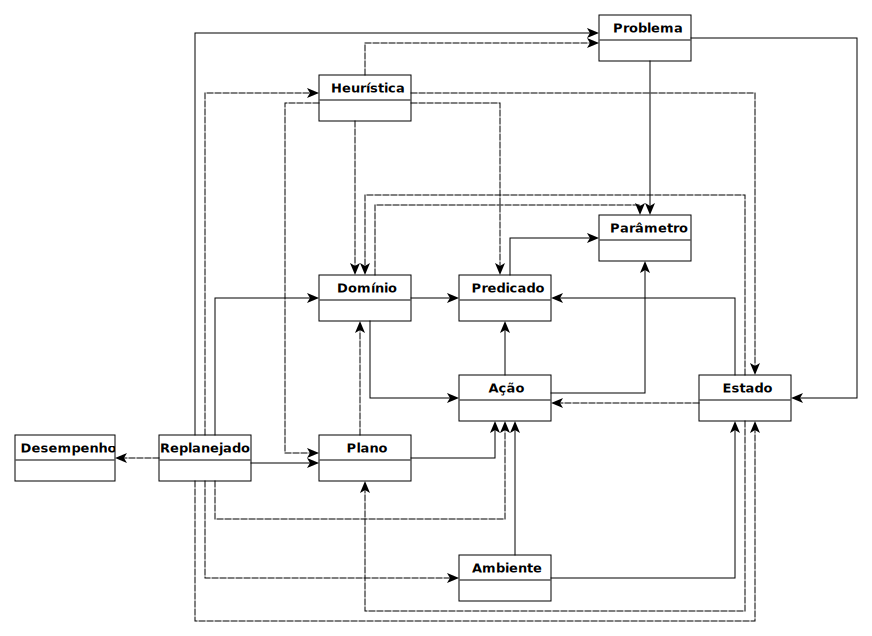
\includegraphics[angle=270,width=1.0\textwidth]{./img/diagrama_classe_sistema.ps}
    \caption[Diagrama de classe do sistema de reparo]{Diagrama de Classe\footnote{Este diagrama segue os conceitos apresentados por \cite{Martin2000}.} do sistema de reparo VHPOP-RE\index{VHPOP-RE}}
  \end{figure}
\end{center}


%%%%%%%%%%%%%%%%%%%%%%%%%%%%%%%%%%%%%%%%%%%%%%%%%%%%%%%%%%%%%%%%%%%%%%%%%

\onehalfspacing
\bibliographystyle{apalike}
\bibliography{diss-bib}

\printindex

\end{document}
